\documentclass[11pt, a4paper]{article}
\usepackage[utf8]{inputenc}
\usepackage[T1]{fontenc}
\usepackage{geometry}
\geometry{left=2.5cm, right=2.5cm, top=2.5cm, bottom=2.5cm}
\usepackage{xcolor}
\usepackage{hyperref}
\usepackage{enumitem}
\usepackage{titlesec}
\usepackage{tcolorbox}
\usepackage{cite}
\usepackage{booktabs}
\usepackage{multirow}
\usepackage{amsmath,amssymb}
\usepackage{pifont}
\usepackage{pgffor}
\usepackage{tocloft}

% Star rating macro for qualitative comparison tables
\newcommand{\stars}[1]{%
  \foreach \i in {1,...,5}{%
    \ifnum\i>#1 \textcolor{gray!40}{$\star$}\else \textcolor{black}{$\star$}\fi
  }%
}

% 目录格式美化（使其更像一本“手册”）
\renewcommand{\cftsecleader}{\cftdotfill{\cftdotsep}}
\hypersetup{
    colorlinks=true,
    linkcolor=blue!60!black,
    filecolor=magenta,      
    urlcolor=cyan,
    pdftitle={LLM Architecture in One Block},
}


\title{
\textbf{
LLM Architecture in One Block: A Survey \\
(Alpha Demo V1)
}
}
\author{Jiaming Ma, Zhe Zhao}
\date{\today}

\begin{document}

\maketitle

\begin{abstract}
The rapid evolution of Large Language Models (LLMs) has led to an overwhelming proliferation of architectural variants. While scaling laws have driven unprecedented performance, the marginal returns of simply scaling standard Transformers are diminishing, and the computational costs are becoming prohibitive. Current literature often presents architectural modifications in isolation, obscuring their underlying mathematical equivalence and coupling effects. To bridge the gap between empirical "alchemy" and systematic "chemistry," this survey serves as a comprehensive design manual for modern LLM architectures. We deconstruct the foundation model into a singular, unified mathematical framework, isolating its search space into six orthogonal dimensions within a single block: Token Mixer, Channel Mixer, Normalization, Position Encoding, Residual Connection, and Module Sequence. Beyond merely cataloging existing methods, we deeply analyze the inductive biases, geometric properties (e.g., manifold constraints in residual streams), and hardware-performance trade-offs of each component. By explicitly decoupling these modules and providing actionable design guidelines, this survey equips researchers and practitioners with a fundamental blueprint for engineering the next generation of efficient, high-performance LLMs.
\end{abstract}

\newpage
\tableofcontents
\newpage

% ================================================================
%  OVERVIEW & MOTIVATION
% ================================================================
\section*{Overview and Motivation}

\subsection*{Why This Survey}

The Transformer architecture~\cite{vaswani2017attention}, introduced in 2017, has become the universal backbone for large language models (LLMs).
In the years since, the research community has produced hundreds of architectural variants---new attention mechanisms, activation functions, normalization schemes, positional encodings, residual topologies, and block layouts---at a pace that makes systematic comparison increasingly difficult.

Existing surveys fall into two categories, neither of which fully serves the practitioner.
On one end, focused reviews cover a single component in depth (e.g., efficient attention~\cite{tay2020efficient}, position encoding~\cite{sajun2024historical}) but cannot capture the coupling effects between components.
On the other end, broad overviews~\cite{shao2024survey, raiaan2024review, kim2025survey} attempt to catalog the entire LLM landscape---spanning data, training, alignment, and deployment---but necessarily sacrifice depth on any individual architectural dimension.
Neither approach provides what an architect needs most: a unified, mathematically grounded framework that isolates each design choice, defines its search space, and analyzes its interaction with every other choice.

This survey fills that gap.
We treat the LLM not as a monolithic system but as a composition of six orthogonal modules within a single repeating block.
Our goal is twofold: (1)~to serve as a practical design manual for LLM architecture, where each section provides enough mathematical depth and empirical evidence to guide real engineering decisions; and (2)~to function as a modern deep learning handbook that is useful beyond the LLM domain---the principles of normalization, residual connectivity, and positional encoding discussed here apply equally to vision transformers, diffusion models, and multimodal architectures.

\subsection*{The Transformer Block: A Six-Dimensional Design Space}

Every modern LLM is built by stacking $L$ near-identical blocks.
We begin from the original Transformer formulation~\cite{vaswani2017attention} and identify the six orthogonal design dimensions within a single block.
The canonical Transformer block computes:
\begin{align}
\label{eq:transformer_block}
% --- Token Mixer (Attention) ---
Q, K, V &= X W^Q,\; X W^K,\; X W^V
  & \text{\small (linear projections)} \notag \\[2pt]
A &= \mathrm{softmax}\!\Bigl(\frac{Q K^\top}{\sqrt{d_k}} + \underbrace{M_{\mathrm{pos}}}_{\text{Position Encoding}}\Bigr)
  & \text{\small (attention matrix)} \\[2pt]
X' &= \underbrace{X + \underbrace{\mathrm{LayerNorm}\bigl(\underbrace{A \, V}_{\text{Token Mixer}}\bigr)}_{\text{Normalization}}}_{\text{Residual Connection}}
  & \text{\small (sub-layer 1)} \notag \\[2pt]
X'' &= \underbrace{X' + \mathrm{LayerNorm}\bigl(\underbrace{\mathrm{FFN}(X')}_{\text{Channel Mixer}}\bigr)}_{\text{Residual Connection}}
  & \text{\small (sub-layer 2)} \notag
\end{align}
where $\mathrm{FFN}(x) = W_2 \,\mathrm{ReLU}(W_1 x + b_1) + b_2$ is the position-wise feed-forward network, and the entire arrangement of normalization, attention, FFN, and residual additions constitutes the \textbf{Module Sequence}.

From this single equation, we extract six orthogonal design dimensions:

\begin{enumerate}[leftmargin=2em, itemsep=4pt]
\item \textbf{Token Mixer} (Section~\ref{sec:token-mixer}): the mechanism by which information flows between positions---$A \cdot V$ in the original formulation. Variants include multi-head attention, grouped-query attention, linear attention, state space models, and hybrid designs.

\item \textbf{Channel Mixer} (Section~\ref{sec:channel-mixer}): the position-wise transformation $\mathrm{FFN}(\cdot)$ that processes each token's representation independently. Variants include gated linear units, mixture-of-experts, and KAN-style alternatives.

\item \textbf{Normalization} (Section~\ref{sec:normalization}): the $\mathrm{LayerNorm}(\cdot)$ operations that stabilize training. Variants include RMSNorm, QKNorm, and normalization-free alternatives.

\item \textbf{Position Encoding} (Section~\ref{sec:position-encoding}): the positional bias $M_{\mathrm{pos}}$ injected into the attention computation. Variants include absolute encodings, RoPE, ALiBi, and context-length extrapolation methods.

\item \textbf{Residual Connection} (Section~\ref{sec:residual-connection}): the identity shortcut $X + F(X)$ that enables gradient flow across layers. Variants include scaled residuals, dense connections, and dynamic depth.

\item \textbf{Module Sequence} (Section~\ref{sec:module-sequence}): the ordering and arrangement of the above components within each block---Pre-Norm vs.\ Post-Norm, serial vs.\ parallel sub-layers, and heterogeneous block designs.
\end{enumerate}

Figure~\ref{fig:taxonomy} provides a visual roadmap of this decomposition.
Each subsequent section begins by formally defining its component in the original Transformer, then systematically surveys the design space of alternatives.

\subsection*{Notation}

To enable precise cross-section comparison, we adopt the following notation consistently throughout this survey:

\begin{table}[h]
\centering
\small
\caption{Unified notation used throughout this survey.}
\label{tab:notation}
\begin{tabular}{cl}
\toprule
\textbf{Symbol} & \textbf{Description} \\
\midrule
$N$ & Sequence length (number of tokens) \\
$d$ & Model (hidden) dimension \\
$d_k, d_v$ & Key and value dimensions per head \\
$d_{\mathrm{ff}}$ & Feed-forward hidden dimension (typically $4d$ or $\tfrac{8}{3}d$ for SwiGLU) \\
$h$ & Number of attention heads \\
$G$ & Number of KV groups in Grouped-Query Attention \\
$L$ & Number of layers (blocks) \\
$l$ & Layer index, $l = 1, \ldots, L$ \\
$W$ & Sliding window size for sparse attention \\
$d_s$ & State dimension for state space models \\
$d_c$ & Latent dimension for MLA compression \\
$E$ & Number of experts in Mixture-of-Experts \\
$k$ & Number of active experts per token (top-$k$) \\
\midrule
$X \in \mathbb{R}^{N \times d}$ & Input token representations to a block \\
$Q, K, V$ & Query, key, value matrices after linear projection \\
$A \in \mathbb{R}^{N \times N}$ & Attention weight matrix \\
$S_t \in \mathbb{R}^{d_k \times d_v}$ & Recurrent state at step $t$ (linear attention / SSM) \\
$x_l$ & Hidden representation at layer $l$ in the residual stream \\
$F_l(\cdot)$ & Sub-layer function at layer $l$ (attention or FFN) \\
\midrule
$\phi(\cdot)$ & Feature map for kernel-based linear attention \\
$G_t$ & Data-dependent gating matrix at step $t$ \\
$\beta_t$ & Data-dependent learning rate for delta-rule updates \\
$\alpha_t$ & Scalar decay factor (SSM / RetNet) \\
$\gamma, \beta$ & Learnable scale and shift in normalization layers \\
$\theta$ & RoPE base frequency parameter \\
\bottomrule
\end{tabular}
\end{table}

\begin{figure}[!h]
    \centering
    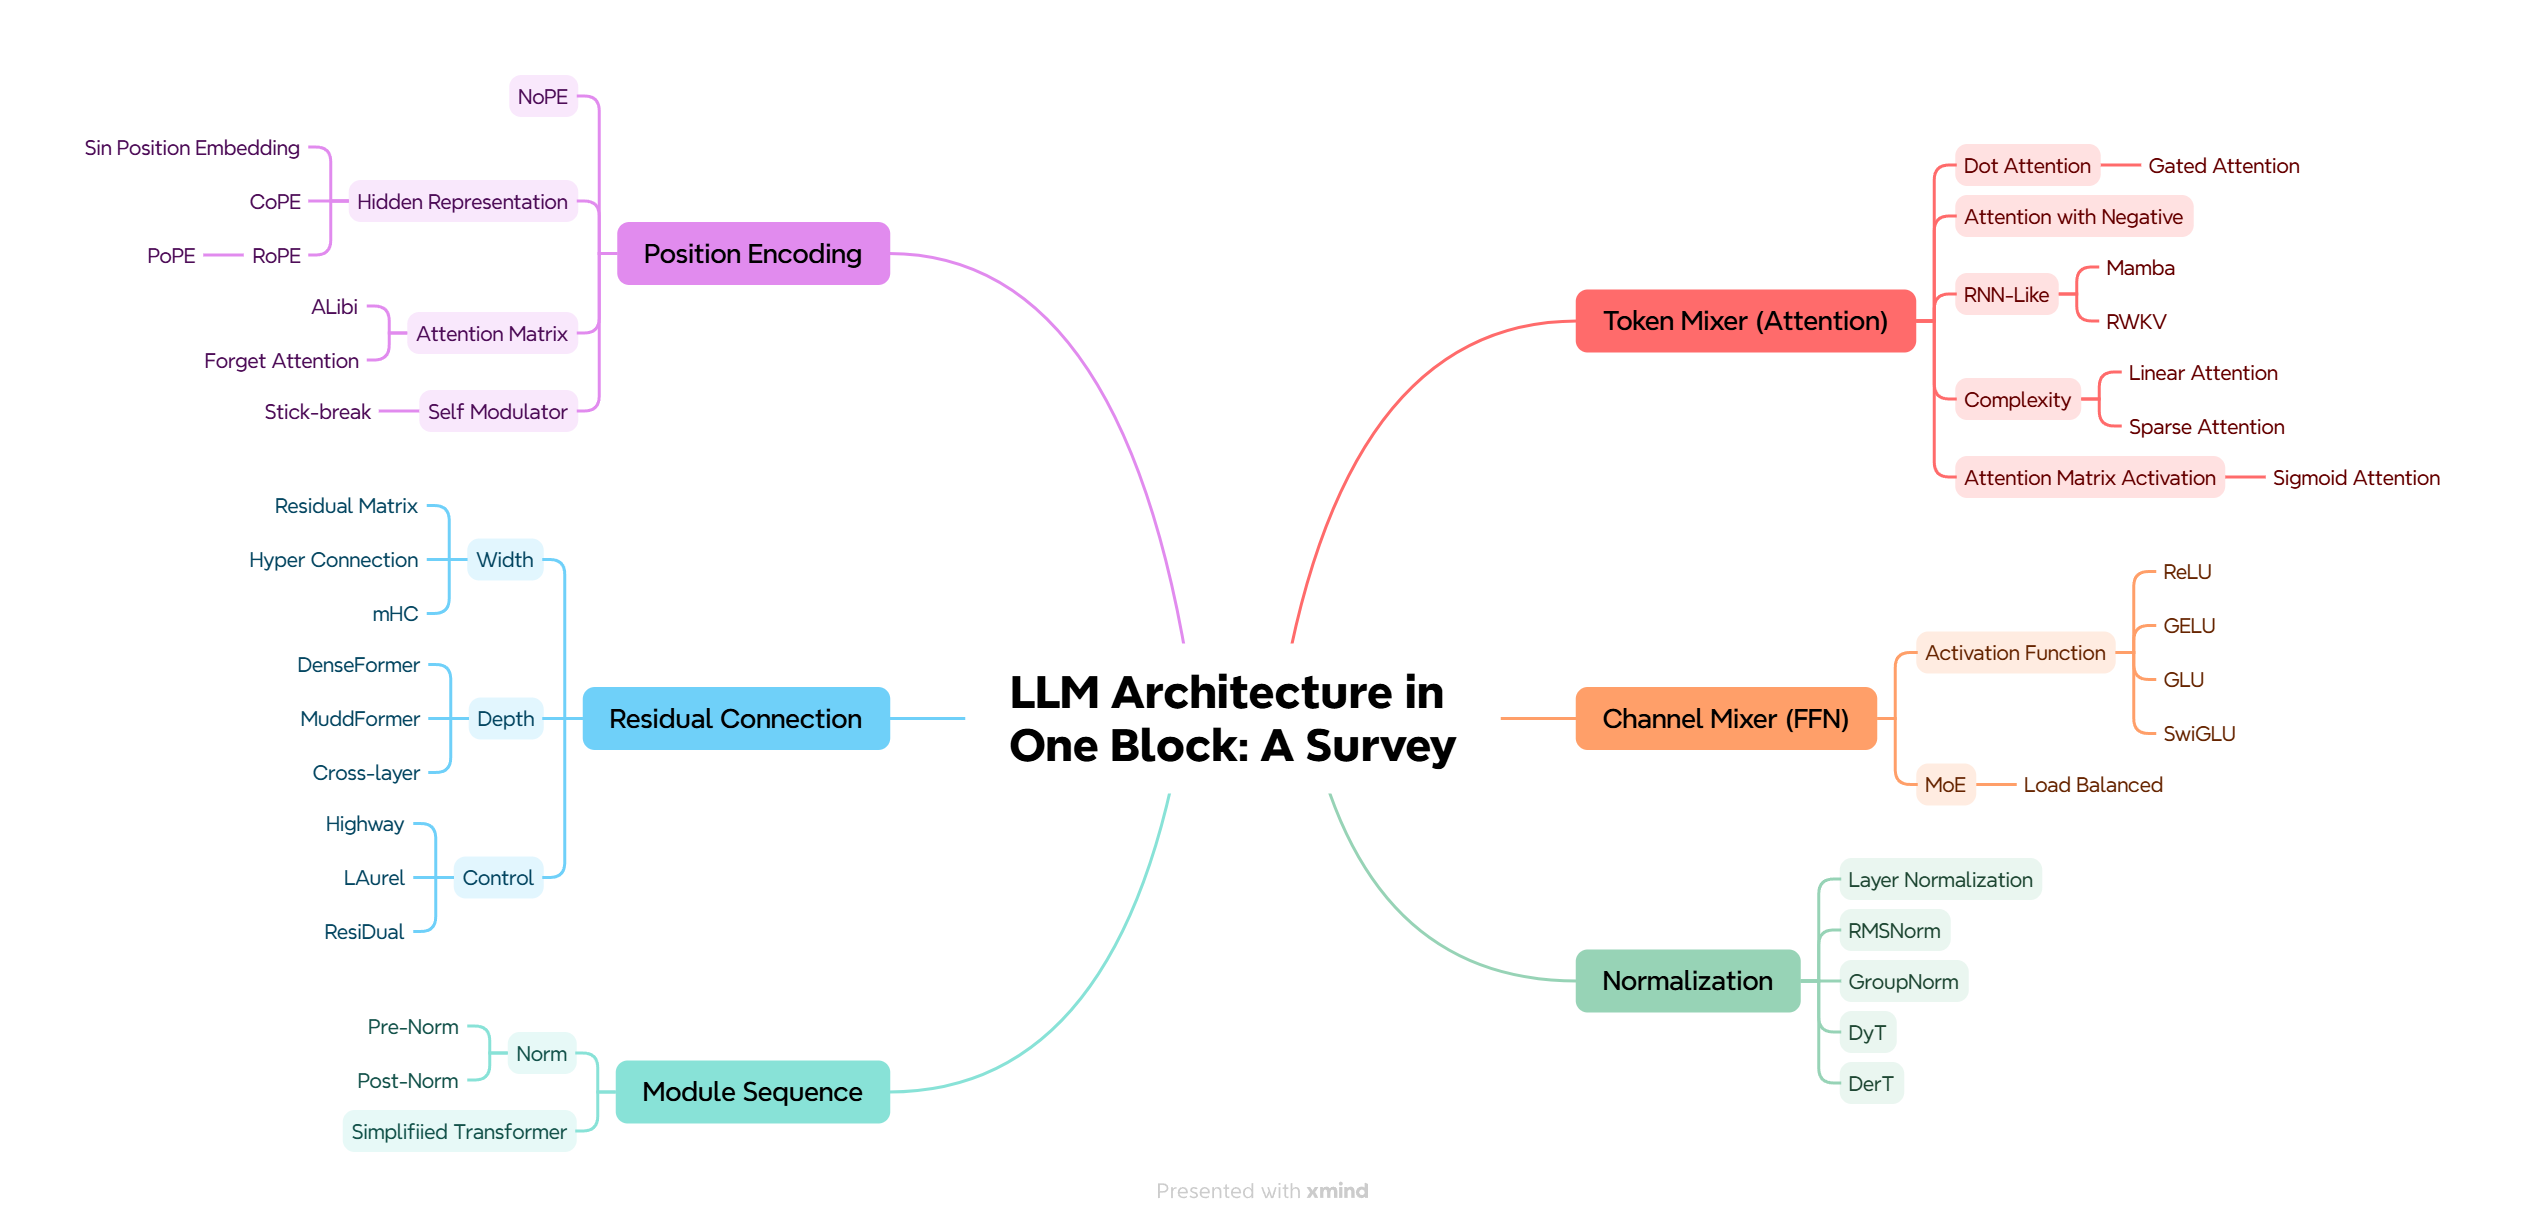
\includegraphics[width=\linewidth]{../Fig/LLM Architecture in One Block A Survey.png}
    \caption{Taxonomy of the six orthogonal design dimensions within a single Transformer block. Each dimension admits independent design choices that compose to define the full architecture. The color coding is used consistently throughout this survey.}
    \label{fig:taxonomy}
\end{figure}

% ================================================================
%  SECTION 1: TOKEN MIXER
% ================================================================
\section{Token Mixer}
\label{sec:token-mixer}

In the original Transformer~\cite{vaswani2017attention}, the token mixer is multi-head scaled dot-product attention:
\begin{equation}
\label{eq:mha_def}
\mathrm{Attention}(Q, K, V) = \mathrm{softmax}\!\Bigl(\frac{Q K^\top}{\sqrt{d_k}}\Bigr) V, \qquad
\mathrm{MHA}(X) = \mathrm{Concat}(\mathrm{head}_1, \ldots, \mathrm{head}_h) W^O,
\end{equation}
where $\mathrm{head}_i = \mathrm{Attention}(X W^Q_i, X W^K_i, X W^V_i)$.
This mechanism allows every token to attend to every other token with data-dependent weights, at $O(N^2 d)$ cost.
All subsequent methods in this section modify one or more aspects of this formulation: the attention kernel (softmax $\to$ linear, gated), the key-value representation (full $\to$ grouped, compressed, shared), the attention pattern (dense $\to$ sparse, local, hybrid), or the entire paradigm (attention $\to$ recurrence, state space).

% =============================================================
% Section: Token Mixer (Attention and Beyond)
% =============================================================
% NOTE: This file begins at \subsection level.
% The \section{Token Mixer} command should appear in main.tex.
% Requires: \usepackage{pifont} in preamble for \ding
% Define \stars macro for qualitative rating (1--5):
% \newcommand{\stars}[1]{\ifcase#1\or\ding{72}\or\ding{72}\ding{72}\or\ding{72}\ding{72}\ding{72}\or\ding{72}\ding{72}\ding{72}\ding{72}\or\ding{72}\ding{72}\ding{72}\ding{72}\ding{72}\fi}
%
% 核心论点: Token Mixer 的演进围绕一个根本性张力展开——
% 训练时的表达力（精确 recall）vs 推理时的效率（吞吐/内存）。
% 所有方法都在这个张力的不同位置做出 trade-off。
%
% 贯穿全文的三条主线:
%   1. Recall-Throughput Trade-off
%   2. 训练/推理二象性（同一数学对象在两个阶段的不同表现）
%   3. 数学收敛（Linear Attn, SSM, Delta Rule, TTT → 统一框架）
% =============================================================

% Helper macro: star ratings for qualitative comparison tables
% Requires: \usepackage{pgffor} and \stars defined in preamble (main.tex)

% ----------------------------------------------------------------
% 引言段：鸟瞰 Token Mixer 的演进
% ----------------------------------------------------------------

The token mixer is the component of a neural language model that governs how information flows between positions in a sequence.
Given a sequence of $N$ token representations $\{x_1, \ldots, x_N\}$, the token mixer produces a new sequence $\{y_1, \ldots, y_N\}$ in which each $y_t$ aggregates information from other positions according to some mixing rule.
The design of this mixing rule---which tokens to attend to, how to weight them, and at what computational cost---has been the single most active axis of LLM architecture research since 2017.

The evolution of token mixers is best understood through a fundamental tension: recall precision versus computational efficiency.
Softmax attention~\cite{vaswani2017attention} achieves near-perfect recall---any token can retrieve any piece of information stored anywhere in the context---but at $O(N^2)$ cost during training and $O(N)$ memory per layer during inference.
Linear attention and state space models reduce these costs to $O(N)$ and $O(1)$ respectively, but compress the entire history into a fixed-size state of $O(d^2)$ capacity, fundamentally limiting their ability to retrieve specific tokens from long contexts.
This tension manifests differently in the two phases of LLM deployment:

\begin{itemize}[nosep,leftmargin=*]
\item \textbf{Training} is compute-bound: the dominant cost is the $O(N^2 d)$ matrix multiplication in attention, but this operation maps efficiently onto GPU tensor cores. The key question is whether the mixing rule can be computed with fewer FLOPs while maintaining model quality.
\item \textbf{Inference} is memory-bandwidth-bound: during autoregressive decoding, each token generation requires loading the entire KV cache from HBM, and the decode throughput is limited by memory bandwidth rather than compute. The key question is how to reduce the per-token state that must be cached and loaded.
\end{itemize}

This asymmetry explains why the field has not converged on a single ``best'' token mixer: methods that excel at training efficiency (e.g., FlashAttention) may not address the inference bottleneck, while methods that minimize inference state (e.g., Mamba) may sacrifice training-time quality.
The most successful production architectures of 2024--2025 resolve this tension through hybrid designs that allocate a small fraction of layers (${\sim}$15\%) to full softmax attention for precise recall, while delegating the majority to efficient alternatives (SSMs, linear attention, or sliding-window attention) for throughput.

A second, deeper trend is the mathematical convergence of seemingly disparate research lines.
The Structured State Space Duality (SSD) framework~\cite{dao2024transformers} revealed that Mamba-2's selective SSM is mathematically equivalent to a specific form of linear attention with data-dependent decay.
The delta rule~\cite{yang2024deltanet}, independently developed in the linear attention community, was shown to be equivalent to one step of online gradient descent on an associative memory---the same update rule as Test-Time Training (TTT)~\cite{sun2024learning}.
These convergences suggest that the space of $O(N)$ token mixers is far more constrained than it appears, and that a unified theoretical framework is within reach.

This section is organized as follows.
We begin with softmax attention and its KV-cache optimizations (\S\ref{subsec:mha}--\ref{subsec:kv-opt}), which define the quality ceiling and the inference bottleneck.
We then examine two strategies for making attention affordable: sparse attention (\S\ref{subsec:sparse}) and hardware-efficient implementations (\S\ref{subsec:hw-attn}).
Next, we turn to the recurrent alternatives---linear attention (\S\ref{subsec:linear-attn}) and state space models (\S\ref{subsec:ssm})---and their mathematical unification (\S\ref{subsec:convergence}).
We discuss hybrid architectures (\S\ref{subsec:hybrid}) as the current pragmatic optimum, attention variants that expand the design space (\S\ref{subsec:attn-variants}), inference-time optimizations (\S\ref{subsec:inference-opt}), and test-time adaptive memory (\S\ref{subsec:ttm}).
We conclude with a synthesis and outlook (\S\ref{subsec:token-mixer-outlook}).


% ================================================================
% 3.1 Softmax Attention: The Quality Ceiling
% ================================================================
\subsection{Softmax Attention: The Quality Ceiling}
\label{subsec:mha}

Multi-head attention (MHA)~\cite{vaswani2017attention} remains, as of mid-2026, the strongest token mixer in terms of raw modeling quality. Understanding why it is so effective---and where it fails---is essential context for every subsequent method in this section.

\paragraph{Mechanism.}
Given an input $X \in \mathbb{R}^{N \times d}$, MHA projects it into queries, keys, and values via learned matrices and computes
\begin{equation}
\text{Attention}(Q, K, V) = \underbrace{\text{softmax}\!\left(\frac{QK^\top}{\sqrt{d_k}}\right)}_{\text{attention map } A \in \mathbb{R}^{N \times N}} V,
\label{eq:mha}
\end{equation}
where $Q = XW^Q$, $K = XW^K$, $V = XW^V$, and the $1/\sqrt{d_k}$ scaling prevents gradient saturation. The multi-head variant partitions the representation into $h$ subspaces:
\begin{equation}
\text{MHA}(X) = \text{Concat}(\text{head}_1, \ldots, \text{head}_h)\, W^O, \quad \text{head}_i = \text{Attention}(XW_i^Q, XW_i^K, XW_i^V).
\end{equation}
Each head can specialize---empirically, different heads learn syntactic dependencies, coreference, positional patterns, and induction (copying) circuits~\cite{olsson2022context}---and the concatenation fuses these diverse relational signals.

\paragraph{Why softmax attention is hard to beat.}
Three properties make softmax attention uniquely powerful:
\begin{enumerate}
\item \textbf{Exact associative recall.} Given a key-value pair $(k_j, v_j)$ stored in context, a query $q_i \approx k_j$ retrieves $v_j$ with arbitrary precision as the softmax temperature decreases. This property is critical for in-context learning, where the model must retrieve and apply input-output mappings from the prompt~\cite{olsson2022context}.
\item \textbf{Data-dependent routing.} The attention map $A$ is a function of the input content, not a fixed pattern. This allows the model to dynamically route information based on semantic relevance, a capability that fixed-pattern sparse attention and position-based methods fundamentally lack.
\item \textbf{Universal approximation.} Sufficiently deep and wide Transformers with softmax attention are universal approximators of continuous sequence-to-sequence functions, and the attention mechanism itself implements a form of Nadaraya--Watson kernel regression with an exponential kernel~\cite{tay2020efficient}.
\end{enumerate}

\paragraph{Computational profile.}
MHA incurs $O(N^2 d)$ FLOPs and $O(N^2 + Nd)$ memory for the attention map. During training, this quadratic cost is amortized across the batch and parallelized efficiently on GPUs; FlashAttention~\cite{dao2022flashattention} reduces the memory to $O(N)$ by never materializing the full $N \times N$ matrix, making sequences up to 8--16K tokens routine. During inference, the cost structure changes fundamentally: the prefill phase (processing the prompt) is compute-bound and benefits from the same parallelism as training, but the decode phase (generating tokens one at a time) is memory-bandwidth-bound. At each decode step, the model must load the entire KV cache ($2LNd_h h$ bytes for $L$ layers) from HBM to compute a single attention vector, yielding an arithmetic intensity of $O(1)$ FLOPs per byte---far below the GPU's compute-to-bandwidth ratio. This decode bottleneck is the primary motivation for every KV-cache optimization discussed in Section~\ref{subsec:kv-opt}.

\paragraph{Known limitations.}
Despite its strengths, softmax attention exhibits several systematic failure modes:
\begin{itemize}
\item \textbf{Attention sink.} LLMs allocate disproportionate attention mass to the beginning-of-sequence token, which acts as a ``garbage collector'' for the probability mass that softmax must distribute~\cite{xiao2023streamingllm}. This wastes representational capacity and complicates KV-cache eviction strategies.
\item \textbf{Non-negative constraint.} Softmax outputs are strictly non-negative, preventing the model from expressing ``do not attend to this token'' signals. Differential Attention~\cite{ye2024differential} addresses this by computing the difference of two softmax maps (Section~\ref{subsec:attn-variants}).
\item \textbf{Rank collapse.} In deeper layers, attention matrices tend toward low-rank structure, reducing the effective diversity of information routing~\cite{dong2021attention}.
\end{itemize}

\paragraph{Decomposing softmax: which properties matter most?}
A finer-grained analysis reveals that softmax imposes three logically independent constraints on the attention weights: (1)~non-negativity ($A_{ij} \geq 0$), (2)~normalization ($\sum_j A_{ij} = 1$), and (3)~sharpening (the exponential function amplifies score differences, concentrating mass on high-scoring keys). These three properties are not equally important. Sigmoid Attention~\cite{ramapuram2024sigmoid} retains non-negativity but discards normalization, and works well when paired with appropriate gating or layer normalization. Polynomial attention variants such as $\mathrm{relu}^2$ discard all three constraints yet remain effective when combined with Frobenius-norm regularization or explicit normalization by the sequence length. The consistent finding across these alternatives is that the sharpening effect---the ability to produce peaked, near-sparse attention distributions---is the most critical property, followed by normalization, with non-negativity being the least essential. This hierarchy explains why linear attention, which lacks the exponential sharpening, suffers the largest quality degradation: it is missing the single most important ingredient.
A complementary perspective comes from the kernel interpretation. The softmax kernel can be decomposed as $\exp(q^\top k) = \exp(\|q\|^2/2) \cdot \exp(\|k\|^2/2) \cdot \exp(-\|q - k\|^2/2)$, revealing that softmax attention is equivalent to a Gaussian (RBF) kernel $\exp(-\|q - k\|^2/2)$ when query and key norms are held constant (as approximately enforced by QK-normalization or RMSNorm). Since the Gaussian kernel corresponds to an infinite-dimensional feature space, this decomposition provides a precise mathematical explanation for why finite-dimensional feature maps in linear attention---which are inherently low-rank---cannot faithfully approximate softmax: they are attempting to approximate an infinite-rank kernel with a finite-rank one.

\paragraph{Current status (2025--2026).}
Full MHA remains the default for models up to $\sim$8K context length. For longer contexts, production models universally adopt either (a)~KV-cache sharing variants (GQA, MLA) that preserve the softmax computation but reduce the cache footprint, or (b)~hybrid architectures that retain softmax attention in a minority of layers. No sub-quadratic method has yet matched softmax attention's recall quality on challenging benchmarks such as multi-hop reasoning and needle-in-a-haystack retrieval at 128K+ context lengths, confirming its role as the quality ceiling against which all alternatives are measured.


% ================================================================
% Pathologies of Softmax Attention
% ================================================================
\subsection{Pathologies of Softmax Attention}
\label{subsec:pathologies}

Despite its dominance, softmax attention exhibits two well-documented pathological behaviors---attention sink and rank collapse---that illuminate fundamental limitations of the $\mathrm{softmax}(QK^\top/\sqrt{d_k})$ formulation and have motivated many of the architectural innovations discussed in subsequent sections.

\subsubsection{Attention Sink}

Xiao et al.~\cite{xiao2023streamingllm} discovered that autoregressive LLMs allocate disproportionate attention mass to the first few tokens in the sequence---regardless of their semantic content. This ``attention sink'' phenomenon has been observed across all major model families (Llama, Mistral, Falcon, Pythia, Qwen) and extends to vision transformers where the CLS token or background patches serve as sinks.

\paragraph{Root cause: the normalization constraint.}
The fundamental origin of attention sinks is the softmax normalization constraint $\sum_j A_{ij} = 1$. When a query $q_i$ has no strong semantic match among the available keys, the model must nonetheless distribute its full probability mass somewhere. The initial tokens, being visible to all subsequent positions under the causal mask, become convenient ``garbage collectors'' for this excess probability mass. Formally, in a trigger-conditional task where the model should sometimes produce a no-op output, softmax attention is mathematically forced to route attention to a sink token; non-normalized alternatives such as ReLU or sigmoid attention can instead output near-zero attention weights, eliminating the need for sinks entirely~\cite{ramapuram2024sigmoid, qiu2025gated}.

\paragraph{Mechanism: the spike-sparse-sink cascade.}
Recent work~\cite{sun2026spike} has dissected the internal mechanism linking massive activations, normalization, and attention sinks in Pre-Norm Transformers. Certain tokens develop anomalously large activation values in specific hidden dimensions (``spikes'') during early FFN layers. When these spiked representations pass through RMSNorm, the large denominator compresses all other dimensions to near-zero, producing a sparse, near-constant vector. This near-constant key vector then attracts disproportionate attention from all queries---not because the token is semantically important, but because its key representation is an approximately fixed point of the softmax computation. The causal structure ensures that the earliest tokens (which accumulate the most spike opportunities) become the dominant sinks.

\paragraph{Functional role.}
Paradoxically, attention sinks serve a beneficial function: by absorbing excess attention mass, they prevent over-mixing of semantic tokens and thereby slow the rank collapse process described below. Removing sink tokens during inference causes immediate model collapse (perplexity explosion), confirming their role as load-bearing architectural elements~\cite{xiao2023streamingllm}. StreamingLLM~\cite{xiao2023streamingllm} exploits this insight by maintaining a fixed cache of $\sim$4 initial ``sink tokens'' plus a sliding window of recent tokens, enabling infinite-length streaming generation with constant memory.

\paragraph{Mitigation strategies.}
Three families of approaches address attention sinks:
\begin{enumerate}[nosep]
\item Preserving sinks: StreamingLLM, H2O~\cite{zhang2023h2o}, and SinkQ retain sink tokens and adapt KV-cache management accordingly.
\item Eliminating the root cause: Sigmoid Attention~\cite{ramapuram2024sigmoid} and Gated Self-Attention~\cite{qiu2025gated} remove the softmax normalization constraint, allowing near-zero attention weights and eliminating the need for sinks. Gated Self-Attention (NeurIPS 2025 Oral) applies a query-dependent sigmoid gate to the attention output, achieving sink-free attention with improved training stability.
\item Canceling the noise: Differential Attention~\cite{ye2024differential} computes $A_1 - \lambda A_2$, where the shared sink component in both attention maps cancels out, producing sparser, more focused effective attention.
\end{enumerate}

\subsubsection{Rank Collapse and Token Uniformity}

The second pathology is the progressive degeneration of attention diversity with network depth.

\paragraph{Doubly exponential rank loss.}
Dong et al.~\cite{dong2021attention} proved that in a pure self-attention network (without residual connections or MLPs), the output representation matrix $X^{(L)}$ converges to a rank-1 matrix---where all token representations become identical---at a doubly exponential rate in the number of layers $L$:
\begin{equation}
\|X^{(L)} - \mathbf{1} v^\top\| \leq C \cdot \exp\!\left(-2^{L}\right),
\label{eq:rank_collapse}
\end{equation}
where $\mathbf{1} v^\top$ is a rank-1 matrix. The mechanism is that softmax attention computes a convex combination of value vectors, and iterated convex combinations converge to a single point. Residual connections and MLPs slow this convergence but do not eliminate it; in practice, the effective rank of hidden representations decreases monotonically with depth in all production LLMs.

\paragraph{Spectral analysis.}
Naderi et al.\ (2025) analyzed the spectrum of the attention matrix $A = \mathrm{softmax}(QK^\top/\sqrt{d_k})$ using random matrix theory, revealing that $A$ generically possesses an outlier eigenvalue separated from the bulk spectrum by a spectral gap. This gap grows with sequence length $N$, accelerating rank collapse in long-context settings and providing a theoretical explanation for the ``lost-in-the-middle'' phenomenon where LLMs struggle to utilize information in the middle of long contexts.

\paragraph{Curse of Depth in Pre-Norm.}
Sun et al.~\cite{sun2025curse} identified a specific mechanism by which Pre-Norm exacerbates rank collapse. Under Pre-Norm, the residual stream variance grows as $\mathrm{Var}(x_l) = \mathrm{Var}(x_0) + \sum_{i=1}^{l} \mathrm{Var}(F_i)$, scaling as $\Theta(L)$. Layer Normalization then compresses this growing signal back to unit variance, causing the relative contribution of each new layer to shrink as $O(1/L)$. The result is that deep-layer Jacobians approach the identity matrix, and the block output $F_l(\mathrm{LN}(x_l))$ contributes negligibly to the residual stream. Empirically, 30--40\% of layers in Pre-Norm LLMs can be pruned with minimal quality degradation~\cite{men2024shortgpt}.

\paragraph{Relationship between the two pathologies.}
Attention sink and rank collapse are not independent phenomena but two manifestations of a shared underlying constraint. Rank collapse arises because softmax attention is inherently a weighted averaging (diffusion) operator; attention sink is the model's learned compensatory mechanism to limit over-diffusion. By concentrating excess attention mass on semantically inert sink tokens, the model reduces the effective mixing rate among semantic tokens, preserving representational diversity at the cost of wasting attention capacity. This perspective explains why removing sink tokens causes model collapse: without the sinks, the full force of the diffusion operator acts on all tokens, accelerating rank collapse to the point of functional failure.

\paragraph{Mitigation approaches.}
Solutions target different aspects of the problem:
\begin{itemize}[nosep]
\item Architectural: Differential Attention~\cite{ye2024differential} introduces negative weights that can counteract diffusion; nGPT~\cite{loshchilov2024ngpt} constrains representations to the unit hypersphere, preventing unbounded variance growth; Shaped Attention~\cite{noci2023shaped} modifies the attention matrix to preserve rank.
\item Normalization placement: Mix-LN~\cite{chen2024mixln} uses Post-Norm for shallow layers and Pre-Norm for deep layers, balancing representation diversity against gradient stability. Peri-LN normalizes at both ends of each sub-layer branch.
\item Depth scaling: DeepNorm~\cite{wang2024deepnet} scales the residual connection by $\alpha = (2L)^{1/4}$ to compensate for depth-induced variance growth. LayerNorm Scaling (LNS) multiplies each LN output by $1/\sqrt{l}$~\cite{sun2025curse}.
\item Pruning: ShortGPT~\cite{men2024shortgpt} identifies and removes redundant deep layers using a Block Influence metric.
\end{itemize}

\paragraph{Open questions.}
Several fundamental questions remain: Can rank collapse be characterized throughout the full training trajectory, not just at initialization? Is there an optimal depth beyond which adding layers yields diminishing returns, and can this be predicted analytically? Do the register tokens observed in Vision Transformers~\cite{darcet2024vision} serve the same function as attention sinks in LLMs? And can a single architectural modification simultaneously eliminate both pathologies without sacrificing the quality advantages of softmax attention?


% ================================================================
% 3.2 Reducing the KV Bottleneck
% ================================================================
\subsection{Reducing the KV Bottleneck: From Head Sharing to Latent Compression}
\label{subsec:kv-opt}

The KV cache is the dominant memory cost during autoregressive inference. For a model with $L$ layers, $h$ heads, and head dimension $d_h$, storing $N$ tokens requires $2Lhd_h N$ values---roughly 160\,GB in FP16 for a 70B-class model at 128K context. Reducing this footprint without degrading generation quality is the most impactful single optimization for LLM deployment. The community has discovered that the KV cache admits compression along at least four orthogonal dimensions---head count, latent rank, layer depth, and numerical precision---and that these dimensions compose multiplicatively.

\paragraph{Head sharing: MQA and GQA.}
Multi-Query Attention (MQA)~\cite{shazeer2019fast} shares a single KV head across all $h$ query heads, reducing the cache by a factor of $h$ (typically 32$\times$). While effective, MQA's aggressive sharing degrades quality on knowledge-intensive tasks. Grouped-Query Attention (GQA)~\cite{ainslie2023gqa} interpolates between MQA and MHA by partitioning $h$ query heads into $G$ groups, each sharing one KV head:
\begin{equation}
\text{GQA}: \quad \text{head}_i = \text{Attention}(Q_i,\; K_{\lceil iG/h \rceil},\; V_{\lceil iG/h \rceil}), \quad i = 1, \ldots, h.
\end{equation}
GQA with $G = 8$ has become the industry default since 2024, adopted by Llama~3~\cite{grattafiori2024llama3}, Mistral~\cite{jiang2023mistral}, Qwen~2.5/3~\cite{yang2024qwen25,yang2025qwen3}, and Gemma~3~\cite{gemma2025gemma3}, achieving quality within 0.5\% of MHA on standard benchmarks while reducing the KV cache by $h/G$ (typically 4$\times$). A key practical contribution is the uptrain procedure: an existing MHA checkpoint can be converted to GQA by mean-pooling KV heads within each group, requiring only $\sim$5\% of the original pretraining compute.

\paragraph{Latent compression: MLA.}
Multi-head Latent Attention (MLA)~\cite{deepseekv2_2024_mla} attacks the rank dimension rather than the head count. It jointly compresses all KV heads into a single low-dimensional latent vector:
\begin{equation}
c_t^{KV} = W^{DKV} h_t \in \mathbb{R}^{d_c}, \quad K_t = W^{UK}\, c_t^{KV}, \quad V_t = W^{UV}\, c_t^{KV},
\label{eq:mla}
\end{equation}
where $d_c \ll hd_h$ (e.g., $d_c = 512$ vs.\ $hd_h = 32{,}768$). Only $c_t^{KV}$ is cached, yielding a 93.3\% reduction in KV-cache size. A technical subtlety is that RoPE positional encoding is incompatible with low-rank compression (the rotation mixes dimensions that the compression tries to separate); DeepSeek resolves this through Decoupled RoPE, which generates a small additional RoPE-embedded key $k^R_t = \text{RoPE}(W^{KR} h_t) \in \mathbb{R}^{d_R}$ concatenated with the compressed key. During attention computation, the up-projection $W^{UK}$ can be absorbed into the query projection, avoiding explicit decompression. MLA has been deployed across the entire DeepSeek series (V2, V3, R1), where it not only matches but exceeds MHA quality---likely because the low-rank bottleneck acts as a regularizer.

\paragraph{Layer sharing: CLA and YOCO.}
Cross-Layer Attention (CLA)~\cite{brandon2024reducing} shares KV caches across every $S$ consecutive layers, exploiting the empirical observation that adjacent layers' KV representations are highly correlated. CLA with stride $S = 2$ halves the total KV footprint while increasing perplexity by only 0.1--0.2 points. YOCO~\cite{sun2024yoco} takes this further with a decoder-decoder architecture: the first $L/2$ layers (the ``self-decoder'') use efficient attention (SWA or linear attention) and produce a single global KV representation, which the remaining $L/2$ layers (the ``cross-decoder'') share via cross-attention. This reduces the KV cache from $O(LNd)$ to $O(Nd)$---a factor-of-$L/2$ saving.

\paragraph{Precision compression.}
Orthogonal to structural sharing, KV caches can be quantized to lower precision. KIVI~\cite{liu2024kivi} quantizes keys to 2-bit and values to 4-bit with per-channel scaling, reducing cache size by 4--8$\times$ with negligible quality loss. SageAttention~\cite{zhang2024sageattention} applies 8-bit quantization to the attention computation itself (both QK and PV matmuls), achieving 2$\times$ speedup on RTX 4090 while maintaining accuracy through per-warp quantization.

\begin{table}[t]
\centering
\caption{KV-cache optimization methods compress along orthogonal dimensions. Compression ratios are relative to standard MHA with FP16 precision.}
\label{tab:kv-cache}
\small
\begin{tabular}{llccc}
\toprule
\textbf{Method} & \textbf{Dimension} & \textbf{Ratio} & \textbf{Quality} & \textbf{Adopted by} \\
\midrule
MQA~\cite{shazeer2019fast}  & Head $\to$ 1    & ${\sim}32\times$  & Moderate drop    & PaLM, StarCoder \\
GQA-8~\cite{ainslie2023gqa} & Head $\to$ $G$  & $4\times$         & $<$0.5\% loss    & Llama 3, Mistral, Qwen, Gemma 3 \\
MLA~\cite{deepseekv2_2024_mla}  & Rank (latent) & ${\sim}57\times$ & Matches MHA & DeepSeek V2/V3/R1 \\
CLA-2~\cite{brandon2024reducing} & Layer sharing   & $2\times$         & $<$0.2 PPL    & Hunyuan-Large \\
YOCO~\cite{sun2024yoco}     & Layer (global)  & ${\sim}L/2\times$ & Comparable    & Research \\
KIVI~\cite{liu2024kivi}     & Precision       & $4{-}8\times$     & Negligible    & Production \\
\bottomrule
\end{tabular}
\end{table}

\paragraph{Composability and future directions.}
The key insight is that these dimensions are orthogonal: GQA (head sharing) $\times$ CLA (layer sharing) $\times$ quantization (precision) can be combined multiplicatively. For example, GQA-8 + CLA-2 + 4-bit quantization yields a combined compression ratio of $4 \times 2 \times 4 = 32\times$ over baseline MHA in FP16. The evolution from MQA to MLA also reveals a deeper trend: the field is moving from parameter sharing (reusing the same KV heads) to information compression (learning a minimal sufficient representation of the KV cache). MLA's success suggests that the intrinsic dimensionality of the KV cache is far lower than its nominal size, and future methods may push this compression further through learned codebook quantization or neural compression.



% ================================================================
% 3.3 Sparse Attention: Exploiting the Sparsity of Attention Maps
% ================================================================
\subsection{Sparse Attention}
\label{subsec:sparse}
The full $N \times N$ attention matrix is empirically highly sparse: in typical language modeling, the vast majority of attention weights are near zero, with each token concentrating its mass on a small subset of informative positions~\cite{child2019generating}. Sparse attention methods exploit this observation by restricting each query to attend only to a subset of key--value positions, reducing the quadratic cost while preserving the softmax computation for the selected pairs. The evolution of sparse attention reveals a recurring lesson: hardware alignment matters more than asymptotic complexity.

\subsubsection{Fixed-Pattern Sparsity (2019--2020)}

\paragraph{Sparse Transformer.}
Child et al.~\cite{child2019generating} introduced the first systematic sparse attention pattern, factorizing the full attention into two complementary heads: a strided head attending to positions $\{t - W, t - 2W, \ldots\}$ at fixed intervals, and a local head attending to the $W$ nearest positions. The union of these two patterns ensures that any two positions are connected within two layers, reducing per-layer cost from $O(N^2)$ to $O(N\sqrt{N})$ with $W = \sqrt{N}$.

\paragraph{Longformer and BigBird.}
Longformer~\cite{beltagy2020longformer} combined sliding-window attention (width $W$) with a small number of global tokens that attend to and are attended by all positions, achieving $O(NW + Ng)$ complexity where $g$ is the number of global tokens. BigBird~\cite{zaheer2020big} added random attention edges and proved that the resulting pattern is a universal approximator of sequence functions and simulates Turing machines, providing the first theoretical justification for sparse attention. However, both methods require custom CUDA kernels for their irregular access patterns, limiting practical adoption.

\paragraph{Why fixed patterns lost.}
Despite theoretical elegance, fixed-pattern methods saw limited production adoption because: (1)~their irregular memory access patterns map poorly onto GPU tensor cores, which are optimized for dense, contiguous matrix multiplications; (2)~FlashAttention~\cite{dao2022flashattention} made exact full attention fast enough for sequences up to 8--16K tokens, eliminating the need for approximation at moderate lengths; and (3)~the patterns are input-independent, wasting compute on positions that happen to fall within the pattern but carry no useful information.

\subsubsection{Production Heterogeneous Patterns (2023--2025)}

The second generation of sparse attention, deployed in production LLMs, abandons the goal of a single universal pattern in favor of heterogeneous configurations that assign different attention types to different layers.

\paragraph{Sliding Window Attention (SWA).}
Mistral 7B~\cite{jiang2023mistral} demonstrated that a uniform sliding window of size $W = 4{,}096$ across all layers achieves competitive quality with full attention for models up to 7B parameters. The key insight is that information propagates across windows through layer stacking: after $L$ layers, the effective receptive field is $L \times W$ tokens. SWA caps the KV cache at $W$ entries per layer via a rolling buffer (circular buffer at index $i \bmod W$), enabling constant-memory streaming inference. Combined with GQA, SWA is the most hardware-friendly sparse variant, requiring only a causal mask modification.

\paragraph{Interleaved local/global attention.}
Gemma~2~\cite{gemma2024improving} interleaves sliding-window and full attention layers in a 1:1 ratio. Gemma~3~\cite{gemma2025gemma3} sharpened this to 5:1 (local-to-global) with distinct RoPE frequencies: $\theta_{\text{local}} = 10{,}000$ for local layers and $\theta_{\text{global}} = 1{,}000{,}000$ for global layers, allowing global layers to encode much longer-range positional information without degrading local resolution. Only ${\sim}$17\% of layers incur quadratic cost, making the architecture substantially more efficient for long contexts.

\paragraph{Temporal convolution on KV.}
Baichuan-M1~\cite{baichuan2025m1} applies a short causal depthwise 1D convolution (kernel size 3--7) over key and value representations before attention, fusing local context into the KV representations themselves. This adds $<$1\% FLOPs while improving fine-grained pattern matching, echoing the short convolution branches in Mamba~\cite{gu2024mamba} but embedded within the attention mechanism.

\subsubsection{Learned Dynamic Sparsity (2024--2025)}

The most recent generation replaces hand-crafted patterns with learned sparsity that adapts to input content, combining the hardware efficiency of block-sparse computation with the expressivity of data-dependent routing.

\paragraph{Native Sparse Attention (NSA).}
Yuan et al.~\cite{yuan2025native} decompose each attention head into three parallel branches: (1)~a compression branch that pools KV blocks into summary tokens via learned linear projections, (2)~a selection branch that uses the compressed representations to route each query to the top-$k$ most relevant KV blocks, and (3)~a sliding window branch for local context. The outputs are combined via a learned gate $g_t = \sigma(W_g [q_t; h_t])$:
\begin{equation}
y_t = g_t^{\text{cmp}} \cdot A_t^{\text{cmp}} + g_t^{\text{sel}} \cdot A_t^{\text{sel}} + g_t^{\text{win}} \cdot A_t^{\text{win}}.
\label{eq:nsa}
\end{equation}
Critically, NSA is trained natively with sparse attention from the start (not distilled from a dense teacher), and achieves quality matching full attention on DeepSeek's internal benchmarks while reducing training FLOPs by $\sim$9$\times$ for 64K sequences.

\paragraph{Mixture of Block Attention (MoBA).}
Lu et al.~\cite{lu2025moba} apply a Mixture-of-Experts-style router to attention: the context is divided into fixed-size blocks, and each query selects the top-$k$ blocks via a lightweight router score $r_{t,j} = q_t^\top \bar{k}_j$ (where $\bar{k}_j$ is the mean key of block $j$). Within selected blocks, standard softmax attention is computed. MoBA is a drop-in replacement for full attention that requires no architectural changes beyond the router, and has been integrated into MoonshotAI's Kimi production system.

\paragraph{The lesson of sparse attention.}
The evolution from Sparse Transformer to NSA reveals three principles: (1)~locality is the strongest prior---every successful method includes a local window component; (2)~hardware alignment trumps asymptotic complexity---$O(NW)$ SWA with contiguous memory access outperforms $O(N \log N)$ Reformer with scattered access; (3)~heterogeneous beats homogeneous---different layers benefit from different sparsity patterns, and the optimal configuration is learned rather than prescribed.


% ================================================================
% 3.4 Hardware--Algorithm Co-Design
% ================================================================
\subsection{Hardware--Algorithm Co-Design}
\label{subsec:hw-attn}

\paragraph{FlashAttention.}
Dao et al.~\cite{dao2022flashattention} introduced FlashAttention, which computes exact softmax attention without ever writing the $N \times N$ attention matrix to HBM. The algorithm tiles the Q, K, V matrices into blocks that fit in SRAM, computes attention within each tile using the online softmax trick (incrementally maintaining the running maximum and normalization denominator), and accumulates the output in-place. The backward pass uses recomputation rather than storing the attention matrix, trading $O(N^2)$ memory for $O(N^2 d^2/M)$ HBM accesses (where $M$ is the SRAM size). This achieves 2--4$\times$ wall-clock speedup over standard attention while reducing memory from $O(N^2)$ to $O(N)$.

\paragraph{FlashAttention-2 and -3.}
FlashAttention-2~\cite{dao2023flashattention2} optimized the work partitioning across GPU thread blocks, achieving 50--73\% of A100 peak FLOPS. FlashAttention-3~\cite{shah2024flashattention3} exploits Hopper (H100) architecture features: warp specialization separates data loading (via TMA) from computation (via WGMMA) into different warp groups, enabling full overlap of memory access and arithmetic; FP8 block quantization with per-block scaling factors enables 1.2 PFLOPS throughput; and incoherence processing (random Hadamard rotation of Q, K before quantization) reduces outlier-induced quantization error. FA-3 achieves 740 TFLOPS in FP16 on H100---75\% of peak, compared to FA-2's 35\% on the same hardware.

\paragraph{FlashLinearAttention.}
Yang et al.~\cite{yang2024gla} extended the IO-aware approach to linear attention and gated linear attention. The key insight is that the chunk-wise parallel form of linear attention (processing the sequence in chunks of size $C$, with intra-chunk parallel attention and inter-chunk recurrent state propagation) maps naturally onto the tiling strategy of FlashAttention. The recurrent state $S_t \in \mathbb{R}^{d_k \times d_v}$ is maintained in SRAM across chunks, and the intra-chunk attention is computed as a dense matrix multiplication on tensor cores. This achieves near-optimal hardware utilization for linear attention variants, closing the gap between their theoretical $O(N)$ complexity and practical throughput.

\paragraph{Lightning Attention-2.}
Qin et al.~\cite{qin2024lightning} proposed a complementary IO-aware algorithm for linear attention that separates intra-block computation (using standard cumulative-sum attention in SRAM) from inter-block computation (using the recurrent KV state), avoiding the need to write intermediate states to HBM. Lightning Attention-2 is the backbone of MiniMax-01's 4M-token context window~\cite{minimax2025}.

\paragraph{The IO-awareness principle.}
The FlashAttention line of work established a principle that now pervades token mixer design: optimize for data movement, not FLOPs. This explains why $O(N^2)$ FlashAttention is faster than $O(N \log N)$ Reformer (whose hash-based routing creates scattered memory accesses), and why chunk-wise linear attention with $O(NC^2)$ intra-chunk FLOPs outperforms theoretically optimal $O(Nd^2)$ recurrent computation (which has low arithmetic intensity). The implication for architecture design is that any new token mixer must be evaluated not by its asymptotic complexity but by its achievable hardware utilization---the fraction of peak FLOPS or peak memory bandwidth it can sustain on target hardware.



% ================================================================
% 3.5 Linear Attention: The Kernel Trick and Beyond
% ================================================================
\subsection{Linear Attention: From Kernel Methods to Gated Recurrences}
\label{subsec:linear-attn}

Linear attention replaces the softmax nonlinearity with a decomposable kernel, enabling a change in the order of matrix multiplications that reduces the complexity from $O(N^2 d)$ to $O(N d^2)$. More profoundly, this algebraic rearrangement reveals that linear attention is mathematically equivalent to a linear recurrent neural network, establishing a deep duality between attention (parallel, quadratic) and recurrence (sequential, linear) that unifies much of the subsequent work in this section.

Standard softmax attention computes $y_t = \sum_j \frac{\exp(q_t^\top k_j)}{\sum_{j'} \exp(q_t^\top k_{j'})} v_j$. If we replace $\exp(q^\top k)$ with a decomposable kernel $\kappa(q, k) = \phi(q)^\top \phi(k)$ for some feature map $\phi: \mathbb{R}^{d_k} \to \mathbb{R}^{d_\phi}$, the attention output becomes:
\begin{equation}
y_t = \frac{\phi(q_t)^\top \sum_{j=1}^{t} \phi(k_j) v_j^\top}{\phi(q_t)^\top \sum_{j=1}^{t} \phi(k_j)} = \frac{\phi(q_t)^\top S_t}{\phi(q_t)^\top z_t},
\label{eq:linear-attn}
\end{equation}
where $S_t = \sum_{j=1}^{t} \phi(k_j) v_j^\top \in \mathbb{R}^{d_\phi \times d_v}$ and $z_t = \sum_{j=1}^{t} \phi(k_j) \in \mathbb{R}^{d_\phi}$. The crucial observation is that $S_t$ and $z_t$ can be maintained as running sums: $S_t = S_{t-1} + \phi(k_t) v_t^\top$, $z_t = z_{t-1} + \phi(k_t)$. This yields two equivalent computation modes:
\begin{itemize}[nosep]
\item \textbf{Parallel mode} (training): compute $\phi(Q) (\phi(K)^\top V)$ as two matrix multiplications in $O(N d_\phi d_v)$ time.
\item \textbf{Recurrent mode} (inference): update $S_t$ and $z_t$ incrementally in $O(d_\phi d_v)$ per step, with $O(1)$ memory per step.
\end{itemize}
This duality---the same mathematical object viewed as a matrix product (parallel) or a recurrence (sequential)---is the foundational insight that connects linear attention to state space models and modern RNNs.

\paragraph{The fast-weight interpretation.}
The recurrent form of linear attention admits a revealing interpretation as a ``fast weight'' system~\cite{schmidhuber1992learning}. The state matrix $S_t \in \mathbb{R}^{d_\phi \times d_v}$, updated via $S_t = S_{t-1} + \phi(k_t) v_t^\top$, is a linear associative memory that is ``trained'' online by each new token through an outer-product update---the same Hebbian learning rule used in classical Hopfield networks. At query time, the retrieval $y_t = \phi(q_t)^\top S_t$ is simply a forward pass through this learned linear model. Under this lens, linear attention implements a fast weight programmer: the slow weights (the projection matrices $W^Q, W^K, W^V$) generate the data that trains the fast weights ($S_t$), which in turn produce the layer output. This perspective establishes a direct theoretical bridge from linear attention to the delta rule (which replaces the Hebbian update with the Widrow--Hoff error-corrective rule) and to Test-Time Training (which generalizes the fast weight to a nonlinear model updated via gradient descent), providing a unified view of the evolutionary trajectory from additive linear attention through DeltaNet to TTT.

\paragraph{Katharopoulos et al.\ (2020).}
The Linear Transformer~\cite{katharopoulos2020transformers} was the first to formalize this duality, using $\phi(x) = \text{elu}(x) + 1$ as the feature map. While the resulting model was 4000$\times$ faster than softmax attention in the recurrent mode, its quality was substantially worse---the elu feature map is a poor approximation of the exponential kernel, and the absence of softmax's sharpening effect produces diffuse, uninformative attention patterns.

\paragraph{Performer (FAVOR+).}
Choromanski et al.~\cite{choromanski2021rethinking} proposed random Fourier features to approximate the softmax kernel: $\phi(x) = \frac{1}{\sqrt{m}} [\exp(w_1^\top x - \|x\|^2/2), \ldots, \exp(w_m^\top x - \|x\|^2/2)]$ where $w_i \sim \mathcal{N}(0, I)$. FAVOR+ provides an unbiased estimate of softmax attention with $O(Nmd)$ complexity, but the variance of the approximation grows with sequence length, and the required number of random features $m$ to maintain accuracy scales unfavorably, limiting practical gains.

\paragraph{The quality gap.}
Vanilla linear attention methods consistently underperform softmax attention by 2--5 perplexity points on language modeling benchmarks. The root cause is the state bottleneck: the matrix $S_t \in \mathbb{R}^{d_\phi \times d_v}$ can store at most $O(d_\phi d_v)$ bits of information about the entire history, regardless of the sequence length $N$. When $N \gg d_\phi d_v$, information must be discarded, and the simple additive update $S_t = S_{t-1} + \phi(k_t) v_t^\top$ provides no mechanism for selective forgetting---new information is superimposed on old, leading to catastrophic interference when key-value associations conflict.

\subsubsection{Gated Linear Attention: Learning to Forget}

The quality gap of vanilla linear attention motivated the introduction of data-dependent gating---a learnable forgetting mechanism that allows the model to selectively erase outdated information from the state.

\paragraph{Gated Linear Attention (GLA).}
Yang et al.~\cite{yang2024gla} introduced a diagonal gating matrix $G_t = \text{diag}(\alpha_t) \in \mathbb{R}^{d_k \times d_k}$ with $\alpha_t = \sigma(W_\alpha x_t) \in (0, 1)^{d_k}$:
\begin{equation}
S_t = G_t \odot S_{t-1} + k_t v_t^\top,
\label{eq:gla}
\end{equation}
where $\odot$ denotes element-wise multiplication broadcast across the value dimension. Each dimension of the state can independently decay at a data-dependent rate, enabling the model to ``forget'' irrelevant associations while retaining useful ones. GLA closes approximately half the quality gap between linear attention and softmax attention, and its chunk-wise parallel form (implemented in FlashLinearAttention) achieves competitive training throughput.

\paragraph{HGRN and HGRN2.}
Qin et al.~\cite{qin2023hgrn, qin2024hgrn2} proposed Hierarchically Gated Linear RNNs, which apply gating at multiple granularities (token-level and segment-level) to capture both fine-grained and coarse-grained temporal structure. HGRN2 further incorporates outer-product state expansion, increasing the effective state capacity.

\subsubsection{The Delta Rule: From Additive to Corrective Updates}

Gating addresses the forgetting problem but not the interference problem: when a new key-value pair $(k_t, v_t)$ has a key similar to an existing association $(k_j, v_j)$ but a different value, the additive update $S_t = S_{t-1} + k_t v_t^\top$ superimposes the new value on the old rather than replacing it. The delta rule provides a principled solution.

\paragraph{DeltaNet.}
Yang et al.~\cite{yang2024deltanet} replaced the additive update with a corrective update inspired by the Widrow--Hoff learning rule:
\begin{equation}
S_t = S_{t-1} + \beta_t (v_t - S_{t-1} k_t) k_t^\top = (I - \beta_t k_t k_t^\top) S_{t-1} + \beta_t v_t k_t^\top,
\label{eq:deltanet}
\end{equation}
where $\beta_t \in (0, 1)$ is a data-dependent learning rate. The term $S_{t-1} k_t$ retrieves the current value associated with $k_t$ in the state; the error $v_t - S_{t-1} k_t$ measures the discrepancy; and the update corrects the state to reduce this error. This ``read-before-write'' mechanism prevents interference: if $k_t$ already maps to $v_t$ in the state, the update is zero. The state transition matrix $(I - \beta_t k_t k_t^\top)$ is a Householder reflection, which Yang et al.\ exploit for efficient parallel training via the compact WY representation of products of Householder matrices.

\paragraph{Gated Delta Networks.}
Yang et al.~\cite{yang2024gated} (NVIDIA) combined the delta rule with Mamba-2's SSD framework and explicit gating, achieving the strongest results among sub-quadratic methods on recall-intensive benchmarks (MQAR, in-context learning). The combination of gating (for forgetting) and delta rule (for interference prevention) addresses both failure modes of vanilla linear attention.

\paragraph{The hierarchy of state updates.}
The progression from additive to gated to delta updates forms a clear hierarchy of increasing expressivity:
\begin{center}
\small
\begin{tabular}{lccc}
\toprule
\textbf{Update rule} & \textbf{Forgetting} & \textbf{Interference prevention} & \textbf{Representative} \\
\midrule
Additive: $S_t = S_{t-1} + k_t v_t^\top$ & \ding{55} & \ding{55} & Linear Transformer \\
Gated: $S_t = G_t \odot S_{t-1} + k_t v_t^\top$ & \ding{51} & \ding{55} & GLA, Mamba \\
Delta: $S_t = S_{t-1} + \beta(v_t - S_{t-1} k_t) k_t^\top$ & \ding{51} & \ding{51} & DeltaNet, GDN \\
\bottomrule
\end{tabular}
\end{center}
Each step up the hierarchy improves recall quality at the cost of more complex parallel training algorithms (cumulative sum $\to$ chunk-wise scan $\to$ Householder WY decomposition).


% ================================================================
% 3.6 State Space Models and Modern RNNs
% ================================================================
\subsection{State Space Models and Modern RNNs}
\label{subsec:ssm}

State space models (SSMs) approach sequence modeling from a different starting point than attention: instead of computing pairwise token interactions, they maintain a fixed-size hidden state $x_t \in \mathbb{R}^{d_s}$ that is updated at each time step via a linear dynamical system. The core trade-off is between the richness of the state update rule and the capacity of the fixed-size state: a richer update can extract more information per token, but the state can store at most $O(d_s^2)$ bits regardless of sequence length.

\subsubsection{From S4 to Mamba: Making SSMs Selective}

\begin{equation}
x_t = \bar{A}\, x_{t-1} + \bar{B}\, u_t, \quad y_t = C\, x_t, \quad \bar{A} = \exp(\Delta A), \quad \bar{B} = (\exp(\Delta A) - I) A^{-1} B,
\label{eq:s4}
\end{equation}
where $A \in \mathbb{R}^{d_s \times d_s}$ is initialized with the HiPPO matrix (designed to optimally compress continuous signals into a fixed-size state) and $\Delta$ is a fixed step size. S4's key innovation was showing that this recurrence can be computed as a global convolution during training: $y = \bar{K} * u$ where $\bar{K}_t = C \bar{A}^t \bar{B}$, enabling $O(N \log N)$ training via FFT while retaining $O(1)$ per-step inference.

\paragraph{Mamba (2023).}
Gu and Dao~\cite{gu2024mamba} made the critical leap from time-invariant to input-dependent (selective) parameters: $B_t = W_B x_t$, $C_t = W_C x_t$, $\Delta_t = \text{softplus}(W_\Delta x_t)$. This selectivity allows the model to dynamically control what information enters the state ($B_t$), what is read out ($C_t$), and at what timescale ($\Delta_t$). The input-dependent $\Delta_t$ is particularly important: large $\Delta_t$ causes rapid decay of the state (forgetting), while small $\Delta_t$ preserves it (remembering). Mamba achieves quality competitive with Transformers of the same size on language modeling while offering $O(1)$ per-step inference and 5$\times$ higher throughput on long sequences.

\paragraph{Mamba-2 and the SSD framework (2024).}
Dao and Gu~\cite{dao2024transformers} revealed a deep structural connection: when the state matrix $A$ is restricted to be a scalar times the identity ($A = -\alpha I$), the selective SSM recurrence becomes:
\begin{equation}
S_t = \alpha_t S_{t-1} + B_t^\top C_t, \quad y_t = S_t q_t,
\end{equation}
which is precisely a form of linear attention with data-dependent scalar decay. This Structured State Space Duality (SSD) unifies SSMs and linear attention under a single framework, and enables a highly efficient ``chunk-wise'' training algorithm: within each chunk of $C$ tokens, the computation is a dense matrix multiplication (leveraging tensor cores); across chunks, the recurrent state is propagated. Mamba-2 achieves 2--8$\times$ faster training than Mamba-1 while matching or exceeding its quality.

\paragraph{Mamba-3 (2025).}
Gu and Dao~\cite{gu2025mamba3} addressed two limitations of Mamba-2: (1)~the restriction to real-valued diagonal $A$ prevents modeling oscillatory dynamics, and (2)~the SISO (single-input single-output) structure limits cross-channel interaction. Mamba-3 introduces complex-valued $A$ matrices (in conjugate-pair form for real-valued computation) with exponential-trapezoidal discretization that correctly handles oscillatory modes, and MIMO (multi-input multi-output) state updates where $B \in \mathbb{R}^{d_s \times d}$ and $C \in \mathbb{R}^{d \times d_s}$ are full matrices rather than vectors. These changes recover the expressivity of S4's complex dynamics while retaining Mamba-2's efficient chunk-wise training.

\subsubsection{Modern RNN Variants}

\paragraph{RWKV (2023--2025).}
The RWKV series~\cite{peng2023rwkv, peng2024eagle, peng2025rwkv7} evolved from a simple exponential-decay attention mechanism (RWKV-4) through channel-wise decay rates (RWKV-5/6) to a full delta-rule update (RWKV-7). RWKV-7's state update is:
\begin{equation}
S_t = \text{diag}(w_t) \cdot S_{t-1} + k_t^\top (a_t \odot v_t) - (S_{t-1} k_t)^\top (b_t \odot k_t),
\end{equation}
where $a_t, b_t$ are data-dependent gates. The third term implements a delta-rule correction, making RWKV-7 mathematically similar to Gated Delta Networks despite being developed independently. This convergence from a completely different research lineage provides strong evidence that the delta rule is a natural endpoint for linear-complexity token mixers.

\paragraph{Griffin and RecurrentGemma (2024).}
De et al.~\cite{de2024griffin} proposed the Real-Gated Linear Recurrent Unit (RG-LRU), a gated linear recurrence operating in the real domain: $h_t = r_t \odot h_{t-1} + \sqrt{1 - r_t^2} \cdot (i_t \odot x_t)$, where $r_t = \exp(-8 \cdot \text{softplus}(\nu) \cdot \sigma(W_a x_t)^2)$ is a data-dependent decay. Griffin interleaves RG-LRU layers with local sliding-window attention layers, and Google released RecurrentGemma (2B/9B) as an open-source implementation. Griffin demonstrated that a well-designed gated linear recurrence can match Transformer quality at the 14B scale when combined with local attention.

\paragraph{xLSTM (2024).}
Beck et al.~\cite{beck2024xlstm} modernized the LSTM with two variants: sLSTM (scalar memory with exponential gating) and mLSTM (matrix memory with a covariance-based update rule). The mLSTM variant maintains a state $S_t \in \mathbb{R}^{d \times d}$ updated via $S_t = f_t S_{t-1} + i_t v_t k_t^\top$, which is structurally identical to gated linear attention (Eq.~\ref{eq:gla}). This convergence of the LSTM lineage with the linear attention lineage further supports the view that gated matrix-valued recurrences are a natural computational primitive.

\subsubsection{The State Bottleneck: A Fundamental Limit}

All methods in this section---linear attention, gated linear attention, delta rule, SSMs, and modern RNNs---share a common limitation: the fixed-size state $S_t \in \mathbb{R}^{d_k \times d_v}$ can encode at most $O(d_k d_v)$ bits of information about the input history, regardless of the sequence length $N$. This state bottleneck manifests as systematic failures on tasks requiring precise retrieval from long contexts:
\begin{itemize}[nosep]
\item \textbf{Needle-in-a-haystack}: retrieving a specific fact embedded in a long document degrades as the document length exceeds the state capacity.
\item \textbf{Multi-query associative recall (MQAR)}: recalling multiple key-value associations simultaneously requires state capacity proportional to the number of associations.
\item \textbf{Multi-hop reasoning}: chaining multiple retrieval steps amplifies the per-step recall error.
\end{itemize}
The state bottleneck is not merely an engineering limitation but an information-theoretic one: no fixed-size state can losslessly compress an arbitrary-length sequence. This fundamental limit is the primary motivation for hybrid architectures (Section~\ref{subsec:hybrid}), which use softmax attention layers to provide exact recall for the information that the efficient layers cannot retain.


% ================================================================
% 3.7 The Great Convergence
% ================================================================
\subsection{The Mathematical Convergence of Sub-Quadratic Methods}
\label{subsec:convergence}

One of the most striking developments of 2024--2025 is the realization that linear attention, state space models, delta-rule networks, and test-time training---developed by largely independent research communities---converge to the same mathematical framework. This convergence is not merely notational; it reflects deep structural constraints on what a fixed-size-state sequence model can compute.

\paragraph{SSD: SSMs are linear attention.}
The Structured State Space Duality~\cite{dao2024transformers} showed that Mamba-2's selective SSM with scalar decay is algebraically identical to linear attention with a data-dependent forgetting gate. Specifically, both compute $y_t = S_t q_t$ where $S_t = \alpha_t S_{t-1} + k_t v_t^\top$, differing only in how $\alpha_t$, $k_t$, $v_t$, and $q_t$ are parameterized. This duality extends to the training algorithm: both can be computed in chunk-wise parallel form with identical computational structure.

\paragraph{Delta rule = online gradient descent = TTT-Linear.}
\paragraph{The hierarchy of recurrent token mixers.}
These convergences organize the space of $O(N)$ token mixers into a clear hierarchy:
\begin{enumerate}[nosep]
\item \textbf{Additive} ($S_t = S_{t-1} + k_t v_t^\top$): Linear Transformer, Performer. No forgetting, no interference prevention.
\item \textbf{Gated} ($S_t = G_t \odot S_{t-1} + k_t v_t^\top$): GLA, Mamba, RWKV-5/6, mLSTM, RetNet. Selective forgetting, but additive interference.
\item \textbf{Delta} ($S_t = S_{t-1} + \beta(v_t - S_{t-1} k_t) k_t^\top$): DeltaNet, GDN, RWKV-7, TTT-Linear. Both forgetting and interference prevention.
\item \textbf{Nonlinear} ($\theta_t = \theta_{t-1} - \eta \nabla_\theta \mathcal{L}(\theta; x_t)$ where $\theta$ parameterizes a nonlinear model): TTT-MLP, Titans. Breaks the $O(d^2)$ state bottleneck by using a neural network as the state.
\end{enumerate}
Each level subsumes the previous one, and the independent convergence of multiple research lines to levels 2--3 suggests that these are natural computational primitives for sequence modeling. Level 4 (nonlinear TTT) is the only approach that can in principle break the state bottleneck, but at the cost of requiring backpropagation through the inner model at each time step---a significant computational overhead that has so far limited its adoption to research settings.



% ================================================================
% 3.7 Hybrid Architectures: The Pragmatic Optimum
% ================================================================
\subsection{Hybrid Architectures: The Pragmatic Optimum}
\label{subsec:hybrid}

The state bottleneck (Section~\ref{subsec:ssm}) implies that no fixed-size-state method can match softmax attention's recall precision on arbitrarily long contexts. Conversely, full softmax attention is prohibitively expensive for long-sequence inference. Hybrid architectures resolve this tension by allocating different token mixer types to different layers, using a small fraction of softmax attention layers for precise recall and a majority of efficient layers (SSM, linear attention, or sliding-window attention) for throughput. The independent convergence of multiple teams on similar mixing ratios suggests that hybrid design is not a temporary compromise but a structurally optimal strategy.

\subsubsection{The Recall--Efficiency Complementarity}

The theoretical motivation for hybrid architectures rests on a complementarity argument: softmax attention and efficient layers have non-overlapping failure modes.
\begin{itemize}[nosep]
\item Softmax attention excels at precise, content-based retrieval (needle-in-a-haystack, multi-hop reasoning, in-context learning) but incurs $O(N)$ KV-cache memory per layer.
\item SSMs and linear attention excel at long-range sequence modeling (language modeling perplexity, summarization) with $O(1)$ per-step state, but fail on tasks requiring exact recall from long contexts.
\end{itemize}
By placing a few attention layers at strategic positions (typically deeper layers), a hybrid model can ``rescue'' the recall failures of the efficient layers while retaining their throughput advantage for the majority of computation.

\subsubsection{Production Hybrid Architectures}

\paragraph{Jamba (AI21, 2024).}
Jamba~\cite{lieber2024jamba_tr} was the first large-scale hybrid, interleaving Transformer and Mamba layers in a 1:7 ratio (one attention layer per seven Mamba layers) with MoE for the FFN. At 52B total parameters (12B active), Jamba fits on a single 80GB GPU with 256K context thanks to the reduced KV-cache footprint---only $\sim$12\% of layers produce KV caches. Jamba demonstrated that the 1:7 ratio preserves Transformer-level quality on standard benchmarks while achieving Mamba-level throughput on long sequences.

\paragraph{MiniMax-01 (2025).}
MiniMax-01~\cite{minimax2025} scaled the hybrid approach to 456B parameters (45.9B active) with a 4M-token context window---the longest among open-weight models at the time of release. It uses Lightning Attention (linear attention with LRPE-d positional encoding) for 7 out of every 8 layers and softmax attention with RoPE for the remaining layer. The 7:1 ratio was determined through extensive ablation: pure linear attention suffered on recall tasks, while 1:1 mixing sacrificed too much efficiency. The softmax layers use standard KV caches (but only 1/8 of layers need them), making 4M-token inference feasible.

\paragraph{Griffin / RecurrentGemma (Google, 2024).}
Griffin~\cite{de2024griffin} interleaves RG-LRU (Real-Gated Linear Recurrent Unit) layers with local sliding-window attention (window size 2048) in a 2:1 ratio. Unlike Jamba and MiniMax-01, Griffin uses local rather than global attention, capping the KV cache at a fixed window size regardless of sequence length. Google released RecurrentGemma~\cite{botev2024recurrentgemma} (2B/9B) as an open-source implementation, demonstrating that Griffin matches Gemma-2B quality with fixed-size inference state.

\paragraph{Zamba2 (Zyphra, 2024).}
Zamba2~\cite{zyphra2024zamba2} introduced shared attention with LoRA differentiation: all attention layers share the same base Q/K/V/O weight matrices, with each instance receiving a unique low-rank adapter $W_i = W_{\text{shared}} + A_i B_i^\top$ (rank 64). This reduces the parameter overhead of attention layers by $\sim$5$\times$ while maintaining per-layer diversity. The Mamba2-to-attention ratio is approximately 6:1, and the shared KV cache further reduces inference memory.

\paragraph{Nemotron-H (NVIDIA, 2025).}
NVIDIA's Nemotron-H~\cite{nvidia2025nemotronh} family (8B and 56B) replaces most self-attention layers with Mamba-2 layers, achieving up to 3$\times$ inference speedup over Qwen-2.5 and Llama-3.1 at equivalent accuracy. The subsequent Nemotron Nano 2 (9B) retains only 4 attention layers out of $\sim$40 total, pushing the efficient-to-attention ratio to $\sim$9:1.

\paragraph{OLMo Hybrid (AI2, 2026).}
OLMo Hybrid~\cite{ai2_2026_olmo_hybrid} replaces the sliding-window attention layers in OLMo~3 with Gated DeltaNet layers, providing the first systematic comparison of GDN vs.\ SWA vs.\ Mamba-2 as the ``efficient component'' in a hybrid. The study found that GDN offers stronger in-context learning than both SWA and Mamba-2, and the resulting 7B hybrid exceeds pure-Transformer OLMo~3 on standard benchmarks.

\paragraph{Qwen3.5 (Alibaba, 2026).}
Qwen3.5 is the first frontier-scale model to adopt Gated DeltaNet as its primary efficient layer: 75\% of layers use GDN (linear attention with delta-rule updates) and 25\% use full softmax attention, yielding a 3:1 ratio. The 397B-total / 17B-active MoE architecture supports 262K-token context with dramatically lower inference cost than a pure-Transformer model of equivalent quality. Qwen3.5's deployment validates that the delta-rule linear attention family has matured from research to production.

\subsubsection{The Convergent Ratio}

\begin{table}[t]
\centering
\caption{Hybrid architecture configurations in production and near-production models. The efficient-to-attention ratio consistently falls in the 3:1 to 9:1 range.}
\label{tab:hybrid}
\small
\begin{tabular}{lllcc}
\toprule
\textbf{Model} & \textbf{Efficient Layer} & \textbf{Attention Type} & \textbf{Ratio (Eff:Attn)} & \textbf{Context} \\
\midrule
Jamba~\cite{lieber2024jamba_tr}       & Mamba          & Global GQA     & 7:1  & 256K \\
MiniMax-01~\cite{minimax2025}         & Lightning Attn & Global Softmax & 7:1  & 4M \\
Griffin~\cite{de2024griffin}           & RG-LRU         & Local SWA      & 2:1  & 8K+ \\
Zamba2~\cite{zyphra2024zamba2}        & Mamba-2        & Shared Global  & 6:1  & 4K \\
Gemma 3~\cite{gemma2025gemma3}        & SWA            & Global Softmax & 5:1  & 128K \\
Nemotron-H~\cite{nvidia2025nemotronh} & Mamba-2        & Global GQA     & $\sim$9:1 & 128K \\
OLMo Hybrid                           & Gated DeltaNet & Global Softmax & 3:1  & 32K \\
Qwen3.5                               & Gated DeltaNet & Global Softmax & 3:1  & 262K \\
\bottomrule
\end{tabular}
\end{table}

The ratios in Table~\ref{tab:hybrid} cluster in the 3:1 to 9:1 range, with a center of gravity around 7:1 for SSM-based hybrids and 3:1 for delta-rule-based hybrids. The lower ratio for delta-rule hybrids likely reflects the stronger recall capability of the delta rule compared to vanilla SSMs, requiring fewer compensating attention layers. The convergence of independent teams on this range---despite different efficient layer choices, model scales, and training data---suggests a robust structural optimum that balances recall precision against inference efficiency.

\paragraph{Layer placement.}
An emerging design principle is that attention layers should be placed in the deeper layers of the network, where the model performs semantic reasoning and long-range integration, while efficient layers handle the shallower layers that primarily capture local syntactic patterns. Nemotron-H and Qwen3.5 both follow this pattern, though systematic ablations of layer placement remain limited.


% ================================================================
% 3.8 Expanding the Attention Design Space
% ================================================================
\subsection{Expanding the Attention Design Space}
\label{subsec:attn-variants}

Beyond the efficiency axis, several lines of work modify the mathematical properties of attention to address specific limitations of the softmax formulation.

\paragraph{Differential Attention (negative weights).}
Ye et al.~\cite{ye2024differential} observed that softmax attention distributes non-trivial probability mass to irrelevant tokens (``attention noise''), because the non-negativity and sum-to-one constraints prevent the model from expressing ``ignore this token.'' Differential Attention computes the difference of two independent softmax maps:
\begin{equation}
\text{DiffAttn}(X) = \bigl(\text{softmax}(Q_1 K_1^\top / \sqrt{d}) - \lambda \cdot \text{softmax}(Q_2 K_2^\top / \sqrt{d})\bigr) V,
\end{equation}
where $\lambda$ is a learnable scalar. The subtraction cancels the shared noise component (analogous to common-mode rejection in differential amplifiers), yielding sparser, more focused attention patterns. Differential Attention reduces hallucination, improves long-context retrieval, and has been adopted in Microsoft's Phi-4-mini. The approach doubles the Q/K projections but halves the head dimension, maintaining comparable parameter count and FLOPs.

\paragraph{Sigmoid attention (removing normalization).}
\paragraph{Gated Self-Attention.}
Qiu et al.~\cite{qiu2025gated} applied a learned output gate $g_t = \sigma(W_g x_t)$ to the attention output, providing fine-grained control over the information flow from the attention layer to the residual stream. This mitigates the attention sink by allowing the model to suppress uninformative attention outputs, and improves training stability in deep networks.

\paragraph{Gated Attention Unit (GAU): fusing attention and FFN.}
Hua et al.~\cite{hua2022transformer} proposed the Gated Attention Unit, which merges the token mixer and channel mixer into a single operation:
\begin{equation}
O = (U \odot \hat{A} V)\, W_O, \quad U = \phi_u(X W_u), \quad \hat{A} = \frac{1}{n}\,\mathrm{relu}^2\!\left(\frac{QK^\top}{\sqrt{s}}\right),
\end{equation}
where $U$ provides an FFN-style gating branch and $\hat{A}$ is a simplified single-head attention map (no softmax, no multi-head split, with $Q, K \in \mathbb{R}^{N \times s}$ at reduced dimension $s \ll d$). The design philosophy is that attention supplies inter-token routing while the element-wise gate $U$ supplies the nonlinear transformation capacity traditionally delegated to the FFN---both functions are accomplished in one fused layer. The gate implicitly provides ``multi-view'' diversity: different dimensions of $U$ selectively amplify or suppress different dimensions of the attention output, functionally substituting for multiple attention heads at lower cost. Empirically, GAU achieves favorable parameter efficiency compared to the standard Attention+FFN pair at BERT-scale, though it has not yet been adopted in large-scale autoregressive LLMs. Its architectural ideas, however, directly influenced Gated Linear Attention (GLA)~\cite{yang2024gla} and the broader trend of incorporating multiplicative gating into efficient token mixers.

\paragraph{Mixture-of-Heads (MoH).}
Wang et al.~\cite{wang2024moh} reformulated multi-head attention as a weighted sum over heads (rather than concatenation) and introduced a router that activates only 50--90\% of heads per token. MoH reduces the effective compute of the attention layer while maintaining or improving quality, and can be applied to both standard and linear attention.


% ================================================================
% 3.9 Inference-Time Optimization
% ================================================================
\subsection{Inference-Time Optimization}
\label{subsec:inference-opt}

Beyond the token mixer design itself, several system-level techniques improve end-to-end inference throughput. These optimizations are largely orthogonal to the choice of token mixer and can be composed with any architecture.

\paragraph{KV-cache eviction and merging.}
During long-context generation, the KV cache can be compressed by selectively removing or merging entries. H2O~\cite{zhang2023h2o} (Heavy-Hitter Oracle) retains only the tokens that have received the highest cumulative attention scores, based on the observation that a small fraction of tokens (``heavy hitters'') account for the majority of attention mass. SnapKV~\cite{li2024snapkv} identifies important tokens by analyzing attention patterns in a small observation window and compresses the cache accordingly. PyramidKV~\cite{cai2024pyramidkv} allocates different cache budgets to different layers (more cache for deeper layers that perform global reasoning, less for shallow layers that focus locally). StreamingLLM~\cite{xiao2023streamingllm} maintains a fixed-size cache by always retaining the initial ``attention sink'' tokens plus a sliding window of recent tokens, enabling infinite-length streaming generation with bounded memory.

\paragraph{Speculative decoding.}
Speculative decoding uses a small, fast draft model to generate $k$ candidate tokens in parallel, which are then verified by the large target model in a single forward pass. Accepted tokens are output directly; rejected tokens trigger re-sampling from the target model's distribution. The key property is that the output distribution is provably identical to the target model's---speculative decoding is a pure latency optimization with no quality degradation. Typical speedups are 2--3$\times$ for well-matched draft-target pairs.

\paragraph{PagedAttention and continuous batching.}
vLLM's PagedAttention~\cite{kwon2023vllm} manages the KV cache as virtual memory pages, eliminating internal fragmentation (which can waste 60--80\% of GPU memory in naive implementations) and enabling efficient continuous batching of requests with different sequence lengths. This system-level optimization provides 2--4$\times$ throughput improvement and has become the standard serving infrastructure for production LLMs.

\paragraph{Interaction with token mixer design.}

% ================================================================
% 3.10 Test-Time Adaptive Memory
% ================================================================
\subsection{Test-Time Adaptive Memory}
\label{subsec:ttm}

Test-Time Training (TTT) layers and their descendants represent a conceptual departure from both attention and recurrence: they replace the fixed-size hidden state with a learnable model whose parameters are updated via gradient descent during inference. This approach is the only known method that can, in principle, break the $O(d^2)$ state bottleneck of linear recurrences.

\paragraph{TTT-Linear and TTT-MLP.}
Sun et al.~\cite{sun2024learning} proposed TTT layers where the hidden state is the weight matrix $W_t$ of an inner model. At each time step, the model performs one step of gradient descent on a self-supervised reconstruction loss:
\begin{equation}
W_t = W_{t-1} - \eta \nabla_W \|W_{t-1} k_t - v_t\|^2 = W_{t-1} - \eta (W_{t-1} k_t - v_t) k_t^\top.
\label{eq:ttt}
\end{equation}
This update is exactly the delta rule (Eq.~\ref{eq:deltanet}), establishing a deep connection: TTT-Linear is DeltaNet, viewed through the lens of online learning rather than signal processing. The key conceptual contribution is that the inner model can be nonlinear: TTT-MLP uses a two-layer MLP as the inner model, with state size $O(|\theta|)$ that can be scaled independently of the input dimension. TTT-MLP outperforms TTT-Linear on long-context tasks (8K+ tokens), demonstrating that nonlinear memory can capture patterns that linear associative memory cannot.

\paragraph{Titans.}
Behrouz et al.~\cite{behrouz2024titans} extended TTT with a three-component architecture: (1)~a long-term memory module (TTT-based neural network updated via gradient descent), (2)~a short-term memory module (sliding-window attention for precise local recall), and (3)~a persistent memory module (learned constant parameters encoding task-general knowledge). The three components are combined via learned gating. Titans introduced surprise-based forgetting: the learning rate $\eta_t$ is modulated by the prediction error $\|M_\theta(k_t) - v_t\|^2$, so that surprising (high-error) tokens are memorized more strongly. Titans achieves state-of-the-art results among sub-quadratic methods on BABILong (1M+ tokens).

\paragraph{In-Place TTT (2026).}
\paragraph{The cost--quality trade-off.}
TTT methods are computationally expensive: each time step requires a backward pass through the inner model, which is $O(|\theta|)$ for TTT-MLP---significantly more costly than the $O(d^2)$ matrix-vector products of SSMs or linear attention. Whether the quality gains justify this cost at production scale remains an open question. The emergence of In-Place TTT suggests a pragmatic middle ground: using TTT selectively (e.g., only for long-context or knowledge-intensive tasks) rather than as the default token mixer.


% ================================================================
% 3.11 Synthesis and Outlook
% ================================================================
\subsection{Synthesis and Outlook}
\label{subsec:token-mixer-outlook}

The evolution of token mixers from 2017 to 2026 can be summarized as a progression through four phases:
\begin{enumerate}[nosep]
\item \textbf{Softmax dominance (2017--2022)}: MHA is the universal token mixer; efficiency improvements come from engineering (FlashAttention) and KV-cache sharing (MQA, GQA).
\item \textbf{The sub-quadratic challenge (2020--2023)}: Linear attention, SSMs, and modern RNNs demonstrate $O(N)$ alternatives, but consistently underperform softmax attention on recall-intensive tasks.
\item \textbf{Hybrid convergence (2024--2025)}: The field converges on hybrid architectures that combine a minority of softmax attention layers with a majority of efficient layers, achieving the quality of full attention at a fraction of the cost.
\item \textbf{Maturation and deployment (2025--2026)}: Hybrid architectures enter production at frontier scale (Qwen3.5, Nemotron, DeepSeek V3.2), the delta rule emerges as the preferred efficient layer, and the mathematical convergence of SSMs, linear attention, and TTT is formalized.
\end{enumerate}

\begin{table}[t]
\centering
\caption{Qualitative comparison of token mixer families. Recall = ability to retrieve specific tokens from long context; Throughput = tokens/second during inference; Long-Ctx = quality maintenance at 100K+ tokens.}
\label{tab:token-mixer-overview}
\small
\begin{tabular}{lccccc}
\toprule
\textbf{Token Mixer} & \textbf{Recall} & \textbf{Throughput} & \textbf{Long-Ctx} & \textbf{Train Eff.} & \textbf{Maturity} \\
Sparse Attention (NSA)     & \stars{4} & \stars{4} & \stars{4} & \stars{3} & Production \\
Linear Attention (GLA)     & \stars{3} & \stars{5} & \stars{5} & \stars{4} & Emerging \\
Delta Rule (GDN)           & \stars{4} & \stars{5} & \stars{5} & \stars{3} & Production \\
SSM (Mamba-2/3)            & \stars{3} & \stars{5} & \stars{5} & \stars{4} & Production \\
Hybrid (Attn + Efficient)  & \stars{5} & \stars{4} & \stars{4} & \stars{4} & Production \\
TTT / Titans               & \stars{4} & \stars{3} & \stars{4} & \stars{2} & Research \\
\bottomrule
\end{tabular}
\end{table}

\paragraph{Open problems.}
Several fundamental questions remain:
\begin{itemize}[nosep]
\item \textbf{Optimal hybrid ratio}: Is the 3:1 to 7:1 efficient-to-attention ratio universal, or does it depend on model scale, task distribution, or training data? Systematic scaling laws for hybrid architectures are lacking.
\item \textbf{Breaking the state bottleneck}: TTT-MLP and Titans demonstrate that nonlinear memory can exceed the $O(d^2)$ capacity of linear states, but at prohibitive computational cost. Can this capacity be achieved more efficiently?
\item \textbf{Native sparse training}: NSA and MoBA show that sparse attention can be trained from scratch, but the optimal sparsity pattern may evolve during training. Adaptive, curriculum-based sparsity schedules remain unexplored.
\item \textbf{Unified architecture search}: With the mathematical convergence of SSMs, linear attention, and delta rule, the design space of efficient layers is increasingly well-understood. Automated architecture search over this unified space---jointly optimizing the mixer type, layer placement, and mixing ratio---is a natural next step.
\item \textbf{Hardware co-evolution}: As custom AI accelerators (TPUs, Trainium, custom ASICs) diverge from the GPU memory hierarchy that shaped FlashAttention, token mixer designs may need to be re-optimized for different compute-to-bandwidth ratios.
\end{itemize}

The trajectory is clear: the token mixer is evolving from a monolithic component (``use softmax attention everywhere'') to a heterogeneous, hardware-aware system in which different layers, different sequence positions, and even different inference phases employ different mixing strategies. The mathematical convergence of sub-quadratic methods provides a principled foundation for this heterogeneity, while the practical success of hybrid architectures at frontier scale confirms its viability.



% ================================================================
%  SECTION 2: CHANNEL MIXER
% ================================================================
\section{Channel Mixer}
\label{sec:channel-mixer}

In the original Transformer~\cite{vaswani2017attention}, the channel mixer is a two-layer position-wise feed-forward network:
\begin{equation}
\label{eq:ffn_def}
\mathrm{FFN}(x) = W_2 \,\mathrm{ReLU}(W_1 x + b_1) + b_2,
\end{equation}
where $W_1 \in \mathbb{R}^{d \times d_{\mathrm{ff}}}$, $W_2 \in \mathbb{R}^{d_{\mathrm{ff}} \times d}$, and $d_{\mathrm{ff}} = 4d$.
This module applies an identical nonlinear transformation to each token independently, accounting for approximately two-thirds of each block's parameters.
Subsequent work modifies the activation function (ReLU $\to$ GELU, SwiGLU), the gating mechanism (ungated $\to$ gated linear units), the capacity allocation (dense $\to$ mixture-of-experts), and the functional form itself (MLP $\to$ KAN).

% ==============================================================================
% Section 2: Channel Mixer (Feed-Forward Networks)
% Full LaTeX body — 8 subsections, no \section command
% ==============================================================================

\subsection{FFN Structure and Activation Functions}
\label{subsec:ffn_activation}

The feed-forward network (FFN) within each Transformer block serves as the channel mixer, applying an identical pointwise nonlinear transformation to every token representation independently.
In the original Transformer architecture~\cite{vaswani2017attention}, the FFN is a two-layer perceptron with a single hidden expansion:
\begin{equation}
\label{eq:vanilla_ffn}
\mathrm{FFN}(x) = W_2 \,\sigma\!\bigl(W_1 x + b_1\bigr) + b_2,
\end{equation}
where $W_1 \in \mathbb{R}^{d \times d_{\mathrm{ff}}}$, $W_2 \in \mathbb{R}^{d_{\mathrm{ff}} \times d}$, and $\sigma$ denotes a pointwise activation function.
The hidden dimension $d_{\mathrm{ff}}$ is typically set to $4d$, so the FFN accounts for roughly two-thirds of each block's parameters.
Because the activation function is the sole source of nonlinearity in this module, its choice fundamentally determines the expressiveness of the per-token feature transformation.

The earliest Transformer models adopted \textbf{ReLU}~\cite{agarap2018deep}, $\mathrm{ReLU}(x)=\max(0,x)$, which is computationally efficient but suffers from the dying neuron problem: units whose pre-activations are consistently negative receive zero gradient and cease to learn.
\textbf{GELU}~\cite{hendrycks2016gaussian} addresses this shortcoming by interpreting activation as a stochastic regularisation expectation, $\mathrm{GELU}(x)=x\,\Phi(x)$, where $\Phi$ is the standard Gaussian CDF.
Its smoothness yields a more favourable optimisation landscape, and GELU became the default in GPT-2 and BERT.
\textbf{Swish} (also called SiLU)~\cite{ramachandran2017searching}, discovered via automated activation search, generalises the sigmoid gate to $\mathrm{Swish}(x)=x\,\sigma(\beta x)$; with $\beta=1$ it coincides with SiLU.
Unlike ReLU, Swish is non-monotonic and everywhere differentiable, properties that empirically benefit deep networks.

A more recent line of work re-examines ReLU-family activations from a sparsity perspective.
\textbf{ReLU$^2$}~\cite{zhang2024relu2} squares the ReLU output, $\mathrm{ReLU}^2(x)=\bigl(\max(0,x)\bigr)^2$, which amplifies the zero region and produces activation sparsity exceeding 90\%.
This hard sparsity---where inactive neurons are exactly zero rather than merely small---enables hardware-level shortcuts that skip zero-valued multiplications, achieving inference speedups comparable to or better than dense SwiGLU networks with negligible quality loss.
The tension between smooth activations that ease training and sparse activations that accelerate inference remains an active area of investigation; emerging approaches such as \textbf{PolyGLU} attempt to reconcile the two by conditioning the activation mode on the input state, breaking the static one-activation-fits-all paradigm.


% ------------------------------------------------------------------------------
\subsection{Gated Linear Units and the Three-Matrix FFN}
\label{subsec:glu}

The introduction of \textbf{Gated Linear Units} (GLU)~\cite{dauphin2017language} marked a structural turning point for the Transformer FFN, replacing the standard two-matrix architecture with a three-matrix design that incorporates multiplicative gating.
In the original formulation, GLU computes
\begin{equation}
\label{eq:glu}
\mathrm{GLU}(x) = \bigl(x W + b\bigr) \otimes \sigma\!\bigl(x V + c\bigr),
\end{equation}
where $\sigma$ is the sigmoid function, $\otimes$ denotes element-wise multiplication, and the right branch acts as a gate that controls the information flow of the left branch.
This mechanism is conceptually analogous to the forget and input gates of LSTMs: one projection generates candidate features while a parallel projection determines which features are retained.

Shazeer~\cite{shazeer2020glu} systematically evaluated GLU variants by substituting the sigmoid gate with different activation functions.
\textbf{ReGLU} uses ReLU, \textbf{GeGLU} uses GELU, and \textbf{SwiGLU} uses Swish:
\begin{equation}
\label{eq:swiglu}
\mathrm{SwiGLU}(x) = \mathrm{Swish}\!\bigl(x W_{\mathrm{gate}}\bigr) \otimes \bigl(x W_{\mathrm{up}}\bigr), \qquad
\mathrm{FFN}_{\mathrm{SwiGLU}}(x) = \bigl(\mathrm{SwiGLU}(x)\bigr) W_{\mathrm{down}}.
\end{equation}
Across matched-parameter comparisons, SwiGLU consistently outperformed both the vanilla FFN and other GLU variants, establishing it as the de facto standard in modern LLMs including LLaMA~\cite{touvron2023llama}, PaLM, and Qwen.
GeGLU, which replaces Swish with GELU in the gate branch, is adopted by models such as Gemma~\cite{gemma2024improving}:
\begin{equation}
\mathrm{GeGLU}(x) = \left(\mathrm{GELU}(x W_1) \odot x V\right) W_2
\label{eq:geglu}
\end{equation}

Because the three-matrix structure introduces an additional projection ($W_{\mathrm{gate}}$, $W_{\mathrm{up}}$, $W_{\mathrm{down}}$ versus the original $W_1$, $W_2$), it increases the raw parameter count from $2 d \cdot d_{\mathrm{ff}}$ to $3 d \cdot d_{\mathrm{ff}}$.
In practice, the hidden dimension is reduced to $d_{\mathrm{ff}} = \tfrac{2}{3} \times 4d \approx \tfrac{8}{3}d$ so that the total parameter budget remains unchanged.
Even under this iso-parameter constraint, the GLU-based FFN consistently surpasses the wider two-matrix FFN, suggesting that the multiplicative interaction provides a qualitatively different---and superior---form of expressiveness.
Theoretically, the gating branch supplies a data-dependent soft mask over the feature space, enabling the network to learn higher-order feature interactions that are difficult to express with additive activations alone.
The gradient flow through the element-wise product also provides a more direct path reminiscent of residual connections, potentially easing optimisation in very deep models.

The three-matrix GLU FFN has become so dominant that the two-matrix design is essentially absent from frontier models released after 2023.
Looking ahead, the gating principle is beginning to diffuse into other modules---gated attention~\cite{qiu2025gated} applies a similar multiplicative control to attention weights---and the interplay between FFN gating and MoE routing (Section~\ref{subsec:moe_routing}) introduces a dual-gating dynamic whose theoretical implications remain largely unexplored.


% ------------------------------------------------------------------------------
\subsection{Mixture-of-Experts: Foundations and Routing Strategies}
\label{subsec:moe_routing}

The Mixture-of-Experts (MoE) paradigm replaces the single dense FFN with a collection of $N$ expert sub-networks, of which only a small subset is activated for each token, thereby decoupling model capacity from per-token computation cost~\cite{jacobs1991adaptive,cai2024survey}.
A lightweight router (or gating network) $g$ maps each token representation $x$ to a distribution over experts; the output is the weighted sum of the selected experts' outputs:
\begin{equation}
\label{eq:moe}
\mathrm{MoE}(x) = \sum_{i=1}^{N} g_i(x)\, E_i(x), \qquad
g(x) = \mathrm{TopK}\!\bigl(\mathrm{softmax}(W_r x + \epsilon),\, k\bigr),
\end{equation}
where $E_i$ denotes the $i$-th expert FFN, $W_r$ is the router's weight matrix, and $\epsilon$ is optional noise injected during training to encourage exploration.

\textbf{Top-$k$ routing}~\cite{shazeer2017outrageously} is the foundational strategy: each token selects the $k$ highest-scoring experts and discards the rest.
The original formulation uses $k{=}2$ with an auxiliary load-balancing loss that penalises uneven expert utilisation.
\textbf{Switch Transformer}~\cite{fedus2022switch} simplified this to $k{=}1$, halving communication overhead but increasing the risk of load imbalance and routing collapse---a failure mode in which a small subset of experts attracts the majority of tokens while others remain underutilised.
To stabilise training, \textbf{ST-MoE}~\cite{zoph2022stmoe} introduced the router z-loss, which penalises large logit magnitudes in the router to prevent numerical instability.

A conceptual inversion of the routing direction was proposed by \textbf{Expert Choice}~\cite{zhou2022mixture}: instead of tokens selecting experts, each expert selects a fixed number of tokens from the global pool.
This guarantees perfect load balance by construction but introduces a new asymmetry---some tokens may be processed by many experts while others are selected by none, potentially causing information loss.
\begin{equation}
S = \mathrm{softmax}(X W_g)^\top \in \mathbb{R}^{E \times N}, \quad \mathcal{T}_e = \mathrm{top\text{-}}k\!\left(S_{e,:}\right) \quad \text{(each expert selects its top-}k\text{ tokens)}
\label{eq:expert_choice}
\end{equation}

More recent work seeks to eliminate the auxiliary loss entirely.
\textbf{Auxiliary-loss-free routing}~\cite{wang2024auxiliary}, adopted by DeepSeek-V3~\cite{liu2024deepseek}, introduces a learnable bias term in the router that dynamically steers tokens from overloaded experts to underutilised ones.
By removing the auxiliary loss, this approach avoids gradient interference with the primary language-modelling objective and simplifies hyper-parameter tuning.
\begin{equation}
b_e \leftarrow b_e + \eta \cdot (\bar{f} - f_e), \quad g(x) = \mathrm{top\text{-}}k\!\left(\mathrm{softmax}(x W_g + b)\right) \quad \text{(bias-corrected routing)}
\label{eq:auxfree}
\end{equation}
\textbf{Soft MoE}~\cite{puigcerver2024soft} takes a different path by eliminating discrete routing altogether: every expert processes a soft weighted combination of all tokens, making the entire module fully differentiable at the cost of losing the computational savings of sparsity.
\textbf{Sigma-MoE}~\cite{hu2024sigma} replaces softmax with per-expert sigmoid scoring, decoupling expert weights from inter-expert competition and improving expert utilisation.
\textbf{ReMoE}~\cite{wang2024remoe} substitutes ReLU for softmax in the router, naturally producing sparse routing weights without an explicit top-$k$ selection step.

Table~\ref{tab:routing_comparison} summarises the key properties of these routing strategies.

\begin{table}[t]
\centering
\caption{Comparison of MoE routing strategies. ``Discrete'' indicates hard token-to-expert assignment; ``Load Bal.'' denotes the mechanism used to encourage balanced utilisation; ``Diff.'' indicates full differentiability.}
\label{tab:routing_comparison}
\small
\begin{tabular}{lccccl}
\hline
\textbf{Strategy} & \textbf{Direction} & \textbf{Discrete} & \textbf{Load Bal.} & \textbf{Diff.} & \textbf{Representative Model} \\
\hline
Top-$k$ + Aux Loss   & Token$\to$Expert & Yes & Aux loss       & No  & GShard~\cite{lepikhin2020gshard} \\
Top-1 (Switch)        & Token$\to$Expert & Yes & Aux loss       & No  & Switch Transformer~\cite{fedus2022switch} \\
Router z-loss         & Token$\to$Expert & Yes & z-loss         & No  & ST-MoE~\cite{zoph2022stmoe} \\
Expert Choice         & Expert$\to$Token & Yes & By design      & No  & EC-MoE~\cite{zhou2022mixture} \\
Aux-Loss-Free Bias    & Token$\to$Expert & Yes & Learned bias   & No  & DeepSeek-V3~\cite{liu2024deepseek} \\
Soft MoE              & Soft (all-to-all) & No  & N/A           & Yes & Soft MoE~\cite{puigcerver2024soft} \\
Sigma-MoE             & Token$\to$Expert & Yes & Sigmoid (ind.) & No  & Sigma-MoE~\cite{hu2024sigma} \\
ReMoE                 & Token$\to$Expert & Yes & ReLU sparsity  & No  & ReMoE~\cite{wang2024remoe} \\
\hline
\end{tabular}
\end{table}


% ------------------------------------------------------------------------------
\subsection{MoE Expert Design: Granularity, Sharing, and Heterogeneity}
\label{subsec:moe_expert_design}

Beyond routing, the design of the experts themselves---their size, number, and structural uniformity---is a critical architectural decision that governs the capacity--efficiency trade-off in MoE models.

\paragraph{Coarse- versus fine-grained experts.}
Early MoE language models employ a coarse-grained design with a small number of full-sized experts.
Mixtral~\cite{jiang2024mixtral} uses 8 experts with top-2 routing, yielding 47B total parameters of which only 13B are active per token.
This design is straightforward to implement and incurs modest communication overhead, but limits the combinatorial diversity of expert combinations.
\textbf{Fine-grained experts}, pioneered by DeepSeekMoE~\cite{dai2024deepseekmoe}, decompose each expert into a smaller FFN and dramatically increase the expert count---DeepSeek-V2~\cite{deepseekv2_2024} uses 160 routed experts with top-6 activation, while DBRX~\cite{databricks2024dbrx} employs 16 experts with top-4 selection.
The combinatorial advantage is substantial: selecting $k$ out of $N$ fine-grained experts yields $\binom{N}{k}$ possible expert combinations, providing far richer functional coverage than a coarse-grained alternative with the same active parameter count.
Pushing this idea to the extreme, He et al.~\cite{he2024million} explore million-scale experts where each expert is reduced to a minimal parameter group, paired with product-key retrieval for efficient routing.

\paragraph{Shared experts.}
DeepSeekMoE introduced the concept of \textbf{shared experts}---one or two experts that are always activated regardless of routing decisions---to capture universal, input-agnostic features common across all tokens.
The routed experts then specialise in domain- or task-specific patterns, mirroring a ``common-mode plus differential'' signal decomposition.
This design was retained in DeepSeek-V2 and V3 and has been influential in the community.
However, Qwen3~\cite{qwen2025qwen3} explicitly removes shared experts, arguing that under a global batch-level load-balancing strategy, routed experts can naturally learn general-purpose representations without a dedicated shared component.
This architectural disagreement---shared versus no-shared---reflects an unresolved question about the optimal division of labour between general and specialised computation.

\paragraph{Heterogeneous experts.}
The standard assumption that all experts share the same architecture is challenged by \textbf{heterogeneous MoE} designs such as ERNIE~4.5~\cite{ernie45_2025}, which assigns different hidden dimensions or depths to different experts.
This allows the model to allocate varying computational budgets to different input patterns, aligning with the intuition that not all tokens require the same complexity of processing.
Heterogeneous designs raise new questions for routing: the router must implicitly learn a mapping between token difficulty and expert capacity, a correspondence that is non-trivial to supervise.
Llama~4~\cite{meta2025llama4} also adopts an MoE architecture at scale, contributing to the growing diversity of expert design philosophies in production systems.


% ------------------------------------------------------------------------------
\subsection{MoE Engineering: Distributed Training and Inference}
\label{subsec:moe_engineering}

Translating the theoretical efficiency of MoE into practical speedups at scale requires addressing a constellation of systems-level challenges, from communication bottlenecks to numerical stability.

\paragraph{Expert parallelism and communication.}
\textbf{Expert Parallelism (EP)}~\cite{lepikhin2020gshard} distributes experts across GPUs so that each device holds a subset of the expert pool.
During forward propagation, an All-to-All communication primitive dispatches each token to the GPU hosting its assigned expert and returns the result.
The communication volume scales as $O(N \cdot d / P)$, where $N$ is the token count, $d$ is the hidden dimension, and $P$ is the number of devices; at large cluster sizes, this overhead can dominate computation.
\textbf{DeepEP}~\cite{deepseek2025deepep} is a purpose-built EP communication library that decomposes the All-to-All into pipelined dispatch and combine stages overlapped with expert computation, exploits NVLink topology-aware routing to minimise cross-node traffic, and supports FP8 communication to halve bandwidth requirements.

\paragraph{Load balancing in practice.}
Beyond routing-level strategies (Section~\ref{subsec:moe_routing}), systems-level load balancing involves setting a capacity factor that caps the maximum number of tokens each expert can process.
Tokens exceeding this capacity are either dropped---incurring information loss---or re-routed to alternative experts.
Switch Transformer~\cite{fedus2022switch} demonstrated that capacity factors of 1.0--1.25 provide a good balance between load uniformity and token coverage.
The auxiliary-loss-free bias approach of DeepSeek-V3 operates at the system level by dynamically adjusting per-expert biases based on running load statistics, achieving near-uniform utilisation without auxiliary gradients.

\paragraph{Mixed-precision training.}
DeepSeek-V3~\cite{liu2024deepseek} achieved a milestone by successfully training a large-scale MoE model with \textbf{FP8 mixed precision} for the expert FFN GEMMs while retaining BF16 for attention and routing computations.
The key enabler is per-group scaling---computing scale factors at a fine granularity (e.g., per 128-element tile) rather than per-tensor---to accommodate the limited dynamic range of E4M3 (maximum representable value $\approx$240).
This approach reduces communication bandwidth by approximately 40\% and accelerates expert computation, with negligible quality degradation.

\paragraph{Training stability.}
MoE training is notoriously prone to instability.
ST-MoE~\cite{zoph2022stmoe} identified that unbounded router logits can trigger gradient explosions and introduced the router z-loss $\mathcal{L}_z = \frac{1}{B}\sum_{i=1}^{B}\bigl(\log \sum_{j=1}^{N} e^{z_{ij}}\bigr)^2$ to regularise logit magnitudes.
Skywork-MoE~\cite{wei2024skywork} and OLMoE~\cite{muennighoff2024olmoe} further document best practices for learning-rate scheduling, expert initialisation, and gradient clipping that are critical for stable convergence.

\paragraph{The inference double penalty.}
While MoE reduces per-token FLOPs during training, inference presents a double penalty~\cite{moe_double_penalty_2026}: (i) all expert parameters must reside in memory even though only a fraction is used per token, resulting in extremely low parameter utilisation; and (ii) distributed inference incurs All-to-All latency proportional to expert count and cluster size.
Consequently, the training efficiency advantage of MoE does not automatically translate to inference efficiency, and bridging this gap---through expert offloading, predictive caching, or specialised hardware---remains one of the most pressing open problems.


% ------------------------------------------------------------------------------
\subsection{Conditional Computation: Beyond Expert Selection}
\label{subsec:conditional_computation}

MoE addresses the question of which experts to activate, but conditional computation asks a more general question: for a given input, how much computation is necessary at all?
This broader framework, first articulated by Bengio~\cite{bengio2013estimating}, posits that large neural networks contain far more capacity than any single input requires, and that learning to dynamically select the appropriate computational sub-graph can decouple model capacity from inference cost without sacrificing quality.

\paragraph{Theoretical foundations.}
Bengio's conditional computation framework rests on three premises: (i)~model capacity and computational cost can be decoupled through sparse activation; (ii)~the routing decision itself must be lightweight, lest the overhead of deciding what to compute negate the savings; and (iii)~the routing policy can be learned end-to-end, potentially via reinforcement learning or straight-through estimators.
The framework generalises MoE---which conditions on expert identity---to conditioning on depth (which layers to execute), width (how many channels to activate), or precision (at what numerical resolution to compute).

\paragraph{Mixture-of-Depths.}
\textbf{Mixture-of-Depths (MoD)}~\cite{raposo2024mixture} operationalises depth-wise conditional computation by training a per-layer binary router that decides, for each token, whether to execute the full Transformer sub-block (attention plus FFN) or to skip it via the residual connection.
A layer-level capacity budget (e.g., 50\% of tokens) constrains the router so that only the most ``informative'' tokens receive full computation.
Empirically, MoD achieves comparable perplexity to the dense baseline while reducing total FLOPs by more than 50\%, validating the hypothesis that natural language tokens exhibit highly non-uniform computational demand---function words such as ``the'' and ``is'' can be processed cheaply, while semantically dense tokens (negations, rare entities) require deeper processing.

\paragraph{Adaptive computation frameworks.}
\textbf{Duo-LLM}~\cite{duollm2024} maintains two parallel FFN pathways per layer---a lightweight and a full-capacity module---and routes each token to the appropriate pathway based on a learned difficulty estimate.
This design systematises the study of per-token compute allocation and can be viewed as a continuous relaxation of the binary skip/compute decision in MoD.
The concept connects to Graves' Adaptive Computation Time (ACT), which allows Universal Transformers to iteratively refine token representations with a variable number of processing steps.

\paragraph{Towards joint depth--width conditioning.}
The combination of MoE (width-level sparsity) and MoD (depth-level sparsity) yields a doubly sparse architecture in which both the set of active experts and the set of active layers are input-dependent.
Early explorations of this combination have appeared in the DeepSeek model family, and the theoretical implications---particularly regarding the interaction between depth-wise and width-wise routing decisions---represent a fertile direction for future work.
The broader vision is a fully adaptive computational graph in which every dimension of the computation (depth, width, precision, even attention span) is conditioned on the input, enabling inference-time compute scaling that allocates resources proportionally to task difficulty.


% ------------------------------------------------------------------------------
\subsection{FFN Sparsity and Post-Training Compression}
\label{subsec:ffn_sparsity}

The observation that large fractions of FFN neurons are inactive for any given input has motivated a rich line of work on exploiting sparsity for inference acceleration, operating at granularities ranging from individual neurons to entire experts.

\paragraph{Contextual sparsity.}
\textbf{Deja Vu}~\cite{liu2023deja} demonstrated that for a given input token, 85--95\% of FFN parameters can be skipped without measurably affecting the output.
Crucially, the set of active neurons varies across inputs---this is contextual sparsity rather than static pruning.
Deja Vu trains a lightweight MLP predictor that, given the previous layer's activation, forecasts which neurons in the current layer will be active, and computes only those neurons.
This approach yields approximately $2\times$ wall-clock speedup on commodity hardware.
The accuracy of the sparsity predictor is the primary bottleneck: overly aggressive prediction causes quality degradation, while conservative prediction limits the achievable speedup.

\paragraph{MoEfication.}
\textbf{MoEfication}~\cite{zhang2022moefication} bridges the gap between dense and sparse architectures by converting a pre-trained dense FFN into a post-hoc MoE structure.
The procedure clusters co-activated neurons into expert groups based on their activation correlation patterns, then trains a lightweight router to select the relevant cluster at inference time.
This enables practitioners to benefit from MoE-style sparsity without the cost and complexity of training an MoE model from scratch, effectively making the dense--MoE boundary a deployment-time rather than design-time decision.

\paragraph{Expert-level pruning.}
In pre-trained MoE models, not all experts contribute equally.
Expert pruning removes underutilised or redundant experts through several criteria: routing frequency (rarely selected experts are pruned), output magnitude (experts with small contributions are discarded), or inter-expert similarity (functionally overlapping experts are merged).
Systematic pruning can reduce the expert count by 30--50\% with minimal quality loss, significantly alleviating the memory footprint problem that plagues MoE inference.

\paragraph{Activation-function-driven sparsity.}
As discussed in Section~\ref{subsec:ffn_activation}, \textbf{ReLU$^2$}~\cite{zhang2024relu2} produces hard zeros for over 90\% of activations, in contrast to the soft near-zero values generated by GELU or SiLU.
Hard sparsity is directly exploitable by hardware: sparse matrix multiplication kernels can skip zero entries entirely, whereas soft sparsity requires thresholding heuristics that introduce approximation error.
This observation has motivated the ``train dense, infer sparse'' paradigm---train with SwiGLU for optimal convergence, then fine-tune or distil into a ReLU$^2$ model for efficient deployment---which is gaining traction as a practical inference optimisation strategy.

\paragraph{Interactions with other compression techniques.}
Sparsity and quantisation are complementary: sparse neurons reduce the number of operations, while quantisation reduces the cost of each operation.
Their joint optimisation---for instance, combining 4-bit weight quantisation with 90\% activation sparsity---has the potential for order-of-magnitude inference speedups, but the interaction effects (e.g., whether quantisation noise disproportionately affects the small set of active neurons) remain insufficiently characterised.


% ------------------------------------------------------------------------------
\subsection{FFN Alternatives: Beyond the MLP Paradigm}
\label{subsec:ffn_alternatives}

The multilayer perceptron---fixed activation functions composed with learnable linear projections---has served as the default channel mixer since the inception of neural networks.
While GLU gating and MoE routing have introduced substantial innovations within this paradigm, a smaller but intellectually significant body of work questions whether the MLP is the only viable design for per-token feature transformation.

\paragraph{Kolmogorov-Arnold Networks.}
\textbf{KAN}~\cite{liu2024kan} draws on the Kolmogorov-Arnold representation theorem, which states that any multivariate continuous function on $[0,1]^n$ can be decomposed as
\begin{equation}
\label{eq:kan}
f(x_1, \ldots, x_n) = \sum_{q=0}^{2n} \Phi_q\!\Biggl(\sum_{p=1}^{n} \phi_{q,p}(x_p)\Biggr),
\end{equation}
where $\Phi_q$ and $\phi_{q,p}$ are univariate functions.
KAN operationalises this theorem by parameterising the univariate functions as learnable B-splines placed on the network's edges rather than its nodes, inverting the standard MLP design in which weights are learnable but activations are fixed.
On low-dimensional scientific computing tasks, KAN exhibits superior approximation efficiency and interpretability compared to MLPs of equivalent size.
However, scaling KAN to LLM-scale models faces formidable obstacles: B-spline evaluation is substantially more expensive than matrix multiplication, efficient GPU kernels for KAN are lacking, and whether KAN's advantages persist in high-dimensional, large-batch regimes is unproven.
Emerging variants---FourierKAN, WaveletKAN, and piecewise-linear approximations---seek to reduce the computational gap while preserving the theoretical appeal.

\paragraph{Adaptive-complexity channel mixing.}
\textbf{Duo-LLM}~\cite{duollm2024} does not replace the MLP but augments it with a parallel lightweight pathway, routing each token to the appropriate complexity level.
This design can be viewed as the channel-mixer analogue of Mixture-of-Depths: rather than skipping entire layers, it adjusts the capacity of the per-token transformation.
The broader implication is that future channel mixers may not be monolithic modules with a single computational profile, but instead offer a continuum of processing intensities tailored to input complexity.

\paragraph{Outlook.}
KAN is more likely to find its niche as a complement to the MLP---deployed in specialised sub-modules requiring high-precision function approximation or interpretability---rather than as a wholesale replacement.
Meanwhile, the convergence of MoE, MoD, and adaptive-complexity designs points toward a unified vision of the channel mixer as a dynamically reconfigurable transformation module.
In this vision, the static notion of ``the FFN'' gives way to a per-token, per-layer decision over what function to apply, how much computation to invest, and which parameters to engage---effectively collapsing expert selection, depth selection, and width selection into a single conditional computation framework.
Realising this vision will require co-design of routing algorithms, hardware accelerators, and training curricula that teach models to allocate computation efficiently from the earliest stages of pre-training.


% ================================================================
%  SECTION 3: NORMALIZATION
% ================================================================
\section{Normalization}
\label{sec:normalization}

In the original Transformer~\cite{vaswani2017attention}, normalization is Layer Normalization applied after each residual addition (Post-Norm):
\begin{equation}
\label{eq:ln_def}
\mathrm{LayerNorm}(x) = \gamma \odot \frac{x - \mu}{\sqrt{\sigma^2 + \epsilon}} + \beta, \qquad
\mu = \frac{1}{d}\sum_{i=1}^{d} x_i, \quad
\sigma^2 = \frac{1}{d}\sum_{i=1}^{d} (x_i - \mu)^2,
\end{equation}
where $\gamma, \beta \in \mathbb{R}^d$ are learnable affine parameters and $\epsilon$ is a small constant for numerical stability.
Normalization controls the scale and distribution of activations, directly determining training stability, maximum trainable depth, and hardware efficiency.
Subsequent work simplifies the computation (LayerNorm $\to$ RMSNorm), changes the placement (Post-Norm $\to$ Pre-Norm), extends normalization into the attention mechanism (QKNorm), and explores normalization-free alternatives (DyT).

% Section 3: Normalization
% Focus: Training stability, optimization landscape, and the evolving understanding of what normalization truly does.

Normalization is arguably the most inconspicuous yet consequential component of the Transformer architecture.
Unlike the attention mechanism, which defines the model's identity, or position encoding, which shapes its inductive biases, normalization operates as a silent guardian of training stability---its presence is rarely questioned, but its absence is immediately catastrophic.
The choice of normalization type, placement, and scope directly determines the maximum trainable depth, hardware efficiency, and scaling behavior of large language models.
From the introduction of Batch Normalization~\cite{ioffe2015batch} in 2015 to the recent emergence of normalization-free architectures such as Dynamic Tanh~\cite{zhu2025transformers} and Dynamic Erf~\cite{chen2025stronger}, the evolution of normalization reflects an ongoing quest to understand what training stability fundamentally requires.
This section traces nine technical threads that collectively map this evolution: from foundational methods to efficient variants, from placement theory to attention-internal constraints, from conditional modulation to holistic architectures, and from automated search to the radical proposal that normalization layers may be dispensable altogether.

%% 3.1 Foundation: BN -> LN -> IN -> GN
\subsection{Foundation: From Batch Normalization to Layer Normalization}

The foundational normalization methods established the principle that normalizing along a chosen set of dimensions stabilizes training by controlling the distribution of activations.
Batch Normalization (BN)~\cite{ioffe2015batch} pioneered this paradigm by computing mean and variance across the batch dimension: given an activation $x_i$, BN computes $\hat{x}_i = (x_i - \mu_\mathcal{B}) / \sqrt{\sigma^2_\mathcal{B} + \epsilon}$ followed by a learnable affine transformation $y_i = \gamma \hat{x}_i + \beta$.
This design enabled higher learning rates, reduced initialization sensitivity, and provided implicit regularization, fueling the success of deep convolutional networks.
However, BN's reliance on batch-level statistics renders it fundamentally incompatible with Transformer-based language models, where variable sequence lengths cause batch statistics to fluctuate dramatically.

Layer Normalization (LN)~\cite{ba2016layer} resolved this incompatibility by normalizing across the feature dimension $d$ within each individual sample, making the computation entirely independent of batch composition.
Given a $d$-dimensional hidden vector $\mathbf{h}$, LN computes:
\begin{equation}
    \text{LN}(\mathbf{h}) = \gamma \odot \frac{\mathbf{h} - \mu}{\sqrt{\sigma^2 + \epsilon}} + \beta, \quad \mu = \frac{1}{d}\sum_{i=1}^{d} h_i, \quad \sigma^2 = \frac{1}{d}\sum_{i=1}^{d}(h_i - \mu)^2,
\end{equation}
where $\gamma, \beta \in \mathbb{R}^d$ are learnable scale and shift parameters.
This formulation provides three decisive advantages for language modeling: (i)~complete independence from batch size, enabling single-sample inference identical to training; (ii)~no need for running statistics, eliminating the train--test discrepancy inherent in BN; and (iii)~compatibility with distributed training without cross-device synchronization.
Instance Normalization~\cite{ulyanov2016instance}, which normalizes per-channel spatial statistics, found its niche in style transfer but has negligible relevance to NLP.
Group Normalization (GN)~\cite{wu2018group} partitions channels into $G$ groups and normalizes within each group, providing a continuous interpolation between Instance Normalization ($G=C$) and Layer Normalization ($G=1$).
GN has recently resurfaced in the Differential Transformer~\cite{ye2024differential}, where it normalizes per-head outputs after the differential attention subtraction---a role that leverages GN's group-wise independence.
The migration from BN to LN established feature-dimension normalization as the default paradigm for sequence models, setting the baseline against which all subsequent innovations are measured.

%% 3.2 Efficient Variants: RMSNorm, ScaleNorm, PowerNorm
\subsection{Efficient Normalization Variants}

Having established Layer Normalization as the standard, a natural question arises: which components of LN are truly necessary?
RMSNorm~\cite{zhang2019root} provides a definitive partial answer by hypothesizing that the re-scaling invariance of LN, rather than its re-centering (mean subtraction), is the key property responsible for training stability.
RMSNorm simplifies LN by eliminating the mean computation entirely:
\begin{equation}
    \text{RMSNorm}(\mathbf{a}) = \frac{\mathbf{a}}{\text{RMS}(\mathbf{a})} \odot \gamma, \quad \text{RMS}(\mathbf{a}) = \sqrt{\frac{1}{n}\sum_{i=1}^{n} a_i^2},
\end{equation}
where $\gamma \in \mathbb{R}^n$ is a learnable gain (no bias $\beta$).
This eliminates one reduction operation and halves the number of learnable parameters from $2d$ to $d$, yielding measured speedups of 7--64\% depending on implementation.
The hypothesis has been substantiated by subsequent geometric analysis~\cite{gupta2024reintroducing}, which reveals that LN's mean subtraction is equivalent to projecting out the component along the all-ones vector $\mathbf{1} = [1, \ldots, 1]^\top$---an irreversible operation that discards information.
Crucially, LLMs trained with RMSNorm (such as LLaMA) naturally learn representations orthogonal to $\mathbf{1}$, rendering the explicit mean subtraction redundant.
RMSNorm is now the de facto standard in virtually all frontier LLMs, including LLaMA~1/2/3, PaLM, Gemma, Qwen, Mistral, and DeepSeek.

ScaleNorm~\cite{nguyen2019transformers} pursues even more extreme simplification: $\text{ScaleNorm}(\mathbf{x}) = g \cdot \mathbf{x} / \|\mathbf{x}\|_2$, using a single global scalar $g$ in place of per-element gains.
This maps all vectors to a hypersphere of radius $g$, foreshadowing the hyperspherical geometry later developed by nGPT~\cite{loshchilov2024ngpt}.
PowerNorm~\cite{shen2020powernorm} takes a different tack, diagnosing why BN fails in NLP---batch statistics fluctuate 3--5$\times$ more in text than in vision---and replacing per-batch variance with an exponential moving average of the quadratic mean.
Despite its theoretical insights, PowerNorm's residual dependence on the batch dimension prevented mainstream adoption.
The trajectory from LN to RMSNorm exemplifies a minimality principle: normalization should retain only the invariance properties that matter, discarding unnecessary computations.

%% 3.3 Normalization Placement: Pre-Norm, Post-Norm, and Beyond
\subsection{Normalization Placement: Pre-Norm, Post-Norm, and Beyond}

Where normalization is placed relative to the sublayer is among the most consequential architectural decisions in Transformer design.
The original Transformer~\cite{vaswani2017attention} adopted \textbf{Post-LN}, applying normalization after the residual addition: $\mathbf{x}_{l+1} = \text{LN}(\mathbf{x}_l + \text{Sublayer}(\mathbf{x}_l))$.
Mean field theory analysis~\cite{xiong2020layer} revealed that Post-LN suffers from large gradient norms near the output layers at initialization, necessitating careful learning rate warm-up.
\textbf{Pre-LN} reverses the order---$\mathbf{x}_{l+1} = \mathbf{x}_l + \text{Sublayer}(\text{LN}(\mathbf{x}_l))$---creating a ``gradient highway'' through which gradients flow unattenuated across arbitrary depth.
Pre-LN eliminates the need for warm-up and has become the default in most modern LLMs, though some evidence suggests Post-LN achieves slightly better final performance when training is successful.

Several proposals seek to combine the stability of Pre-LN with the performance of Post-LN.
\textbf{Sandwich-LN}~\cite{ding2021cogview} applies normalization both before and after the sublayer, originally developed to suppress NaN losses during FP16 training of the 4B-parameter CogView model; Gemma~2~\cite{gemma2024improving} later adopted this pattern with Pre+Post RMSNorm.
\textbf{DeepNorm}~\cite{wang2024deepnet} scales the residual connection by a constant $\alpha > 1$: $\mathbf{x}_{l+1} = \text{LN}(\alpha \cdot \mathbf{x}_l + f(\mathbf{x}_l))$, coupled with theoretically derived initialization scaling.
\begin{equation}
x_{l+1} = \mathrm{LN}\!\left(\alpha \cdot x_l + F_l(x_l)\right), \quad \alpha = (2L)^{1/4},\; \text{init: } W \sim \mathcal{N}(0, \beta^2), \; \beta = (8L)^{-1/4}
\label{eq:deepnorm}
\end{equation}
This enabled training a 1,000-layer Transformer (2,500 sublayers), demonstrating that a 200-layer 3.2B model can outperform a 48-layer 12B model by 5 BLEU points---evidence that depth is an efficient scaling axis.
\textbf{Sub-LN / MAGNETO}~\cite{wang2022magneto} pushes normalization inside sublayers at a finer granularity, inserting additional LN between projections within both attention and FFN blocks, achieving uniform improvements across language, vision, speech, and multimodal tasks.
\textbf{Peri-LN}~\cite{kim2025periln} applies normalization at both ends of the sublayer while keeping the residual path direct: $\mathbf{x}_{l+1} = \mathbf{x}_l + \text{LN}_2(f(\text{LN}_1(\mathbf{x}_l)))$, achieving controlled linear variance growth $\text{Var}(\mathbf{x}_{l+1}) \approx \text{Var}(\mathbf{x}_l) + O(1)$.

More recent work pushes beyond fixed placement entirely.
\textbf{GeoNorm}~\cite{li2026geonorm} replaces traditional normalization with geodesic updates on a representation manifold, $\mathbf{h}_{l+1} = \text{Exp}_{\mathbf{h}_l}(\alpha_l \cdot \mathbf{v}_l)$, unifying Pre-LN and Post-LN as special cases of tangent-space transformations and manifold projections, and introducing a normalization schedule analogous to learning rate schedules.
\textbf{SiameseNorm}~\cite{wang2025siamesenorm} adopts a dual-stream architecture maintaining both a Pre-Norm stream (for gradient stability) and a Post-Norm stream (for representation quality) with shared parameters, fusing their outputs at inference---though at the cost of nearly doubled computation.
A unifying perspective comes from particle interaction theory~\cite{karagodin2025normalization}, which models token representations as interacting particles on a hypersphere: self-attention acts as an inter-particle force, while normalization acts as a velocity regulator, with different placements corresponding to different velocity--stability trade-offs.

%% 3.4 Attention-Internal Normalization
\subsection{Attention-Internal Normalization}

While traditional normalization operates at the sublayer level, the attention mechanism's internal computations harbor their own sources of numerical instability---most critically, the unbounded growth of $QK^\top$ dot-product logits as model depth and hidden dimension increase.
\textbf{QK-Norm}~\cite{henry2020query} addresses this by $\ell_2$-normalizing the query and key vectors before the dot product:
\begin{equation}
    \hat{Q} = Q / \|Q\|_2, \quad \hat{K} = K / \|K\|_2, \quad \text{Attn} = \text{softmax}\!\left(g \cdot \hat{Q}\hat{K}^\top\right) V,
\end{equation}
where $g$ is a per-head learnable scalar initialized to $\sqrt{d_k}$.
By constraining logits to cosine similarities in $[-1, 1]$ and then rescaling by $g$, QK-Norm fundamentally eliminates logit explosion and prevents softmax saturation.
This technique has been adopted by Gemma~2/3, Qwen~3, OLMo~2, and Chameleon, though it is notably incompatible with DeepSeek-V3's Multi-Latent Attention, which does not materialize full Q and K tensors.

\textbf{Logit soft-capping}~\cite{gemma2024improving} provides a complementary output-side constraint: $\text{logits} \leftarrow c \cdot \tanh(\text{logits} / c)$, bounding logits within $(-c, +c)$.
Gemma~2 employs attention logit capping at $c = 50$ and final logit capping at $c = 30$, creating a multi-layered defense.
In the Differential Transformer~\cite{ye2024differential}, the subtraction of two softmax maps produces outputs whose values are no longer bounded by $[0, 1]$, necessitating GroupNorm~\cite{wu2018group} applied per attention head to restore controlled activation scales; the $(1 - \lambda_{\text{init}})$ rescaling factor further aligns gradient flow.
Recent work on Lp-QKNorm~\cite{lopez2026enhanced} generalizes L2 normalization to arbitrary $L_p$ norms, demonstrating that different values of $p$ induce different attention space geometries, though validation remains limited to small-scale settings.
Attention-internal normalization has transitioned from an optional enhancement to a necessary safeguard at scale, with Gemma~2's triple-layered protection (Pre+Post RMSNorm, QK-Norm, soft-capping) representing the current state of engineering practice.

%% 3.5 Conditional and Adaptive Normalization
\subsection{Conditional and Adaptive Normalization}

Standard normalization treats the affine parameters $\gamma$ and $\beta$ as static, shared across all inputs.
Conditional normalization makes these parameters functions of an external conditioning signal, transforming the normalization layer into a lightweight but powerful mechanism for signal injection.
This idea traces back to FiLM (Feature-wise Linear Modulation)~\cite{perez2018film}, which modulates visual features with question embeddings in visual question answering via $\text{FiLM}(\mathbf{x}) = \gamma(\mathbf{c}) \odot \mathbf{x} + \beta(\mathbf{c})$.
AdaNorm~\cite{xu2019understanding} explored input-dependent normalization strength within Transformers, adapting the degree of normalization based on the ``difficulty'' of the input, though it did not achieve widespread adoption.

The decisive breakthrough came with \textbf{adaLN-Zero}~\cite{peebles2023scalable} in the Diffusion Transformer (DiT).
Here, conditioning signals (timestep embedding and class embedding) are passed through a shared MLP to dynamically generate six parameter sets per block---scale $\gamma$, shift $\beta$, and gate $\alpha$ for both the attention and FFN sublayers:
\begin{equation}
    (\gamma_1, \beta_1, \alpha_1, \gamma_2, \beta_2, \alpha_2) = \text{MLP}\!\left(\text{embed}(t) + \text{embed}(c)\right),
\end{equation}
\begin{equation}
    \text{output} = \mathbf{x} + \alpha \odot \text{Sublayer}\!\left(\gamma \odot \frac{\mathbf{x} - \mu}{\sigma} + \beta\right).
\end{equation}
The zero-initialization of the MLP's output layer ensures that each block initially acts as the identity function, providing training stability analogous to Fixup~\cite{zhang2019fixup}.
adaLN-Zero achieved state-of-the-art FID of 2.27 on ImageNet 256$\times$256 and significantly outperformed both cross-attention and in-context conditioning.
Its influence is pervasive: Stable Diffusion~3, Flux, and Sora all build upon the DiT architecture with adaLN conditioning.
This success establishes normalization layers as the canonical interface for conditioning signal injection in generative models, a pattern that may extend to cross-modal fusion in multimodal architectures.

%% 3.6 Holistic Normalization Architectures
\subsection{Holistic Normalization Architectures}

While the preceding methods treat normalization as a localized operation at specific positions, a more radical approach elevates normalization to a global architectural principle.
\textbf{nGPT}~\cite{loshchilov2024ngpt} constrains all vectors in the network---embeddings, hidden states, query/key/value projections, MLP weights, and output weights---to lie on the unit hypersphere via $\ell_2$ normalization.
Layer updates become spherical interpolations:
\begin{equation}
    \mathbf{h}_{l+1} = \text{Normalize}\!\left(\mathbf{h}_l + \alpha_l \cdot \left(f_l(\mathbf{h}_l) - \mathbf{h}_l\right)\right),
\end{equation}
where $\alpha_l$ is a learnable step size and the final normalization reprojects onto the sphere.
Equivalently, constraining all vectors to the unit hypersphere and using spherical linear interpolation:
\begin{equation}
\hat{x}_l = \frac{x_l}{\|x_l\|_2}, \quad x_{l+1} = \mathrm{slerp}\!\left(\hat{x}_l,\, \hat{F}_l(\hat{x}_l),\, \alpha_l\right)
\label{eq:ngpt}
\end{equation}
Because both Q and K are normalized, attention logits are naturally cosine similarities in $[-1, 1]$, eliminating the need for separate QK-Norm.
Critically, nGPT contains no traditional LayerNorm or RMSNorm layers---normalization is an intrinsic property of the representation space rather than an extrinsic correction.
The key geometric insight is that in unconstrained Euclidean space, a substantial fraction of optimizer updates merely change vector norms without altering directions, wasting computation.
The hyperspherical constraint eliminates this redundant degree of freedom, and nGPT achieves 4--20$\times$ reduction in steps to reach equivalent loss, though large-scale validation beyond nanoGPT remains pending.

\textbf{Gemma~2}~\cite{gemma2024improving} pursues the opposite philosophy---maximal redundancy for maximal robustness.
It deploys normalization at multiple levels simultaneously: Pre+Post RMSNorm at the sublayer level, QK-Norm at the attention input level, and logit soft-capping at both the attention and final output levels.
This multi-layered defense eliminates loss spikes across 2B, 9B, and 27B parameter scales.
\textbf{UnitNorm}~\cite{zhao2024unitnorm}, developed independently for time-series Transformers, applies pure $\ell_2$ normalization $\mathbf{x}/\|\mathbf{x}\|_2$ with zero additional parameters, addressing token shift and attention sparsity problems specific to temporal data.
Its convergence with nGPT's hyperspherical philosophy from entirely different problem domains suggests that projection onto the unit sphere may be a broadly effective inductive bias.
nGPT and Gemma~2 thus represent two polar philosophies of normalization design---geometric minimalism versus engineering defense-in-depth---and future architectures may need to navigate between these extremes.

%% 3.7 Automated Normalization-Activation Search
\subsection{Automated Normalization-Activation Search}

Normalization and activation functions are typically adjacent operations in Transformer blocks, and their functional roles---value range control and nonlinear transformation---exhibit significant overlap.
\textbf{EvoNorm}~\cite{liu2020evolving} challenges the assumption that these should be separately designed by defining a search space of primitive operations (addition, multiplication, division, sigmoid, variance, mean) and using evolutionary search to discover unified normalization-activation layers.
The search yielded two notable architectures: EvoNorm-B0 (batch-dependent), $\text{EvoNorm-B0}(\mathbf{x}) = \mathbf{x} \cdot \sigma(\mathbf{x} / v(\mathbf{x}))$, where sigmoid provides gating and variance provides normalization; and EvoNorm-S0 (batch-independent), which replaces variance with group standard deviation.
Both surpass their hand-designed counterparts (BN+ReLU and GN+ReLU, respectively) on ImageNet and COCO, and the layers discovered on small proxy tasks transfer directly to larger benchmarks.

The primary limitation of EvoNorm is its exclusive validation on convolutional architectures.
Whether the search paradigm can discover superior alternatives to the RMSNorm+SwiGLU combination now standard in Transformer FFN blocks remains an open question.
The search space would need to incorporate Transformer-specific primitives (e.g., attention logits, residual paths) and scale to architectures where evaluation cost is substantially higher.
Nevertheless, EvoNorm demonstrates that the joint normalization-activation design space is far from fully explored, and that automated methods can discover non-obvious functional compositions that outperform human intuition.

%% 3.8 Normalization-Free Architectures
\subsection{Normalization-Free Architectures}

If the essential functions of normalization can be achieved through other means---careful initialization, gradient clipping, or bounded activation functions---then normalization layers themselves may be unnecessary.
This line of inquiry began with \textbf{Fixup}~\cite{zhang2019fixup}, which showed that zero-initializing the last layer of each residual branch (making each block initially an identity function) controls variance growth and enables BatchNorm-free training of deep ResNets.
\textbf{T-Fixup}~\cite{huang2020tfixup} extended this to Transformers by scaling $W_V$ and $W_O$ by $(9N)^{-1/4}$ and initializing FFN output weights near zero, completely removing all LayerNorm layers and warm-up schedules while matching standard Transformer performance on machine translation.
\textbf{NFNet}~\cite{brock2021high} decomposed BN's implicit functions into two explicit mechanisms: Scaled Weight Standardization for controlling forward-pass signal variance, and Adaptive Gradient Clipping (AGC)---$G \leftarrow \lambda \frac{\|W\|_F}{\|G\|_F} G$ when $\|G\|_F / \|W\|_F > \lambda$---for constraining backward-pass update magnitude.
This achieved 86.5\% top-1 on ImageNet without any normalization.

The most disruptive recent development is \textbf{Dynamic Tanh (DyT)}~\cite{zhu2025transformers}, which observed that the input--output mapping of trained LayerNorm layers empirically resembles an S-shaped curve and proposed a direct replacement:
\begin{equation}
    \mathrm{DyT}(x) = \gamma \odot \tanh(\alpha \, x) + \beta, \quad \alpha \in \mathbb{R}^d \text{ (learnable per-dimension)}
    \label{eq:dyt}
\end{equation}
where $\alpha$ is a per-layer learnable scalar and $\gamma, \beta$ are per-channel parameters.
As a purely element-wise operation with no reduction, DyT is maximally hardware-friendly and matches normalization performance across ViT, LLaMA, DiT, and wav2vec~2.0.
\textbf{Dynamic Erf (Derf)}~\cite{chen2025stronger} refines this insight by analyzing the critical role of saturation speed: erf saturates more slowly than tanh (Gaussian decay $O(e^{-x^2})$ versus exponential decay $O(e^{-2|x|})$), preserving gradients at larger magnitudes---at $|x|=2$, the erf derivative is approximately 26$\times$ larger than tanh's.
Derf uses $\text{Derf}(\mathbf{x}) = \text{erf}(\alpha \mathbf{x} + s)$ and consistently outperforms both DyT and standard normalization across all tested architectures.
These results challenge a decade of normalization research by suggesting that the essential function of normalization may not be statistical standardization at all, but rather bounded nonlinear compression---a function that any sufficiently well-behaved sigmoidal mapping can provide.

%% 3.9 Frontier Directions
\subsection{Frontier Directions: Hardware Co-Design, Optimizer Coupling, and Outlier Dynamics}

The most recent research reveals that normalization is not an isolated architectural component but is deeply entangled with hardware precision, optimizer design, and emergent activation dynamics.

\paragraph{FP8 training and normalization.}
The transition to FP8 arithmetic exposes a fundamental tension: normalization layers that stabilize training in full precision can become error amplifiers in low precision~\cite{zhang2025whylowprecision}.
The mechanism involves a positive feedback loop: low-rank similarity structures emerge in attention, concentrating information in few dimensions; quantization errors in these critical dimensions are then amplified by RMSNorm's division (an underestimated RMS causes global over-scaling) and softmax's exponentiation, eventually triggering loss spikes.
FOG~\cite{sun2025fog} addresses this architecturally by mandating QK-Norm (bounding attention logits within FP8's dynamic range) and inserting additional RMSNorm at strategic positions to control FFN intermediate activation scales, achieving all-FP8 GEMM computation with 40\% throughput improvement over BF16.
The activation kurtosis serves as a practical monitoring metric: lower kurtosis indicates more FP8-friendly distributions.

\paragraph{Optimizer--normalization coupling.}
The Muon optimizer~\cite{jordan2025muon} reveals an unexpected duality: by orthogonalizing momentum updates via SVD decomposition ($\theta_t = \theta_{t-1} - \text{lr} \cdot UV^\top$), Muon implicitly maintains the spectral condition of weight matrices, controlling activation norms through the backward pass rather than the forward pass.
This is dual to normalization layers, which control forward-pass activation scales.
The combination of Muon (backward spectral control) with DyT/Derf (forward bounded compression) raises the intriguing possibility of completely eliminating traditional normalization from both passes---though this remains an open research direction.

\paragraph{Outlier--normalization symbiosis.}
Recent analysis~\cite{bondarenko2026outlier} reveals that the massive activations and attention sinks observed in trained Transformers are not pathological artifacts but functional features co-evolved with normalization.
When a single activation $x_k \gg x_i$ dominates, RMSNorm effectively becomes $\hat{x}_i \approx x_i \cdot \sqrt{d} / |x_k| \cdot \gamma_i$---the outlier's magnitude controls the effective scale of all other dimensions.
Removing normalization eliminates outliers but degrades performance; clipping outliers while retaining normalization is equally harmful.
This symbiosis has practical implications for quantization, which must preserve outlier functionality rather than suppress it, and provides a new interpretation of DyT/Derf as alternative rescaling mechanisms that do not depend on outlier co-evolution.

\paragraph{Module-level hybrid normalization.}
\textbf{HybridNorm}~\cite{chen2025hybridnorm} abandons the assumption that a single normalization strategy should apply uniformly, instead assigning QKV-Norm to attention modules (controlling logit range and output scale) and Post-Norm to FFN modules (preserving gradient signal quality).
This module-specific strategy proves effective for both dense Transformers and sparse Mixture-of-Experts architectures, where Post-Norm helps maintain consistent output scales across different experts.

\vspace{0.5em}
These frontier directions converge on a deeper insight: the essence of normalization may not reside in any specific network layer, but in maintaining certain invariants during training---spectral conditioning, norm boundedness, or value-range compression.
These invariants can be enforced through normalization layers (the traditional approach), bounded activation functions (DyT/Derf), optimizer design (Muon), architectural constraints (nGPT), or combinations thereof.

%% Comparison Table
\begin{table}[t]
\centering
\caption{Comparison of normalization methods for Transformer-based models. ``Norm Dim.''\ indicates the dimension along which statistics are computed. ``Params'' denotes learnable parameters per normalized dimension $d$. ``Reduction Ops'' counts the number of statistical reduction operations (mean, variance, or RMS) per forward pass.}
\label{tab:norm_comparison}
\small
\begin{tabular}{lccccl}
\toprule
\textbf{Method} & \textbf{Norm Dim.} & \textbf{Params} & \textbf{Reduction Ops} & \textbf{Year} & \textbf{Adoption} \\
\midrule
BatchNorm~\cite{ioffe2015batch} & Batch & $2d$ & 2 (mean, var) & 2015 & CNNs only \\
LayerNorm~\cite{ba2016layer} & Feature & $2d$ & 2 (mean, var) & 2016 & BERT, GPT-2 \\
RMSNorm~\cite{zhang2019root} & Feature & $d$ & 1 (RMS) & 2019 & LLaMA, Qwen, Mistral \\
ScaleNorm~\cite{nguyen2019transformers} & Feature & 1 & 1 (L2 norm) & 2019 & Limited \\
QK-Norm~\cite{henry2020query} & Per-head Q,K & 1/head & 1 (L2 norm) & 2020 & Gemma 2/3, Qwen 3 \\
adaLN-Zero~\cite{peebles2023scalable} & Feature & $6d$/block & 2 (mean, var) & 2023 & DiT, SD3, Sora \\
nGPT~\cite{loshchilov2024ngpt} & All vectors & $\alpha$/layer & 1 (L2 norm) & 2024 & Experimental \\
DyT~\cite{zhu2025transformers} & Element-wise & $2d{+}1$ & 0 & 2025 & Experimental \\
Derf~\cite{chen2025stronger} & Element-wise & 2 & 0 & 2025 & Experimental \\
\bottomrule
\end{tabular}
\end{table}


% ================================================================
%  SECTION 4: POSITION ENCODING
% ================================================================
\section{Position Encoding}
\label{sec:position-encoding}

In the original Transformer~\cite{vaswani2017attention}, positional information is injected by adding fixed sinusoidal embeddings to the input:
\begin{equation}
\label{eq:pe_def}
\mathrm{PE}(t, 2i) = \sin\!\bigl(t / 10000^{2i/d}\bigr), \qquad
\mathrm{PE}(t, 2i+1) = \cos\!\bigl(t / 10000^{2i/d}\bigr),
\end{equation}
and the model input becomes $X + \mathrm{PE}$.
This absolute encoding provides a unique representation for each position but does not generalize to sequence lengths unseen during training.
Subsequent work shifts from absolute to relative encodings (RoPE, ALiBi), from additive to multiplicative injection, and from fixed to learnable and context-dependent schemes, with a central focus on length extrapolation.

%%%%%%%%%%%%%%%%%%%%%%%%%%%%%%%%%%%%%%%%%%%%%%%%%%%%%%%%%%%%
%% Section 4: Position Encoding
%%%%%%%%%%%%%%%%%%%%%%%%%%%%%%%%%%%%%%%%%%%%%%%%%%%%%%%%%%%%
%% \section moved to main.tex
\label{sec:position_encoding}

The self-attention mechanism of the Transformer is inherently permutation-invariant: given a set of input tokens, the output is unchanged by any reordering unless positional information is explicitly injected. Position encoding (PE) is the architectural component responsible for providing this sequential inductive bias. Since the sinusoidal encoding of Vaswani et al.~\cite{vaswani2017attention}, the design of PE has traversed a rich trajectory---from absolute to relative, from fixed to learnable, from data-agnostic to data-dependent, and from one-dimensional to multi-dimensional. We organize this section along ten methodological branches that trace this evolution.

%% 4.1 NoPE
\subsection{No Position Encoding (NoPE)}
\label{subsec:nope}

A provocative starting point for any discussion of PE is whether explicit positional encoding is necessary at all. In decoder-only architectures, the causal attention mask $M_{\text{causal}}$ already encodes a weak ordering: each token attends only to its predecessors, and the resulting lower-triangular structure provides implicit positional cues.

Kazemnejad et al.~\cite{kazemnejad2023impact} systematically compared NoPE, sinusoidal PE, RoPE, and ALiBi on five synthetic arithmetic and reasoning tasks. NoPE achieved the best or near-best length generalization on four of the five tasks, demonstrating that causal attention can recover both absolute and relative position information. The Llama~4 architecture~\cite{llama4_2025} operationalizes this insight in its iRoPE design, interleaving NoPE layers (with global attention and no positional encoding) with RoPE layers at a 1:3 ratio. The NoPE layers are not constrained by training-time context length and, combined with inference-time temperature scaling, enable a 10M-token context window.

DroPE~\cite{gelberg2026drope}, proposed by Sakana AI, takes this idea further: models are pre-trained with standard RoPE, after which the positional encoding is simply removed at inference time with only 100--1,000 steps of short-context recalibration fine-tuning. The underlying insight is that positional encoding serves as ``scaffolding'' during training and can be safely discarded once positional awareness has been absorbed into the model weights.

%% 4.2 Absolute PE
\subsection{Absolute Position Encoding}
\label{subsec:ape}

Absolute PE assigns a unique encoding vector to each position and adds it element-wise to the input embedding. The sinusoidal encoding of Vaswani et al.~\cite{vaswani2017attention} uses frequency-decomposed sine and cosine functions:
\begin{equation}
  \mathrm{PE}_{(\mathrm{pos},2i)} = \sin\!\bigl(\mathrm{pos}/10000^{2i/d}\bigr), \quad
  \mathrm{PE}_{(\mathrm{pos},2i+1)} = \cos\!\bigl(\mathrm{pos}/10000^{2i/d}\bigr),
  \label{eq:sinusoidal_pe}
\end{equation}
where each dimension corresponds to a sinusoid of a different wavelength ranging from $2\pi$ to $10000 \cdot 2\pi$. A key mathematical property is that, for a fixed offset $k$, $\mathrm{PE}_{\mathrm{pos}+k}$ can be expressed as a linear function of $\mathrm{PE}_{\mathrm{pos}}$, theoretically facilitating the learning of relative positions. Learned PE~\cite{gehring2017convolutional}, adopted by BERT and GPT-2, replaces fixed sinusoids with trainable embedding vectors but cannot generalize to unseen lengths.

CAPE~\cite{likhomanenko2021cape} bridges absolute and relative PE via data augmentation: during training, positions are globally shifted ($\beta \sim \mathcal{U}(-\delta,\delta)$) and scaled ($\alpha \sim \mathcal{U}(1-\epsilon,1+\epsilon)$), yielding augmented encodings $\mathrm{PE}(\alpha p + \beta)$ that implicitly encode relative distance. Although absolute PE has largely been superseded by RoPE in LLMs, its multi-frequency design directly inspired the frequency basis $\theta_i = 10000^{-2i/d}$ of RoPE.

%% 4.3 Attention Bias
\subsection{Relative Position Encoding via Attention Bias}
\label{subsec:attention_bias}

Rather than modifying input representations, attention bias methods inject positional information directly into the attention logits. Shaw et al.~\cite{shaw2018self} introduced clipped relative position embeddings into the attention score computation. Transformer-XL~\cite{dai2019transformerxl} decomposed the attention score into four terms---content-content, content-position, global content bias, and global position bias---using fixed sinusoidal encodings processed through learnable projection matrices.

T5 Relative Bias~\cite{raffel2020exploring} adopted a minimalist scalar-bias approach with logarithmic distance bucketing (32 buckets total), encoding the inductive bias that nearby positions require fine-grained distinction while distant positions can be grouped. DeBERTa~\cite{he2021deberta} introduced a disentangled attention mechanism separating content and position representations with dedicated projection matrices. ALiBi~\cite{press2021train} eliminated all learnable parameters by adding a head-specific linear bias $m \cdot [-(i-1),\ldots,-1,0]$ to the attention logits, where slopes follow the geometric series $m_h = 2^{-8h/H}$. While ALiBi achieves ``train short, test long'' generalization and was adopted by BLOOM and MPT, its fixed linear decay limits extrapolation to 2--4$\times$ training length.

\begin{equation}
A_{ij} = \frac{q_i^\top k_j}{\sqrt{d_k}} - m_h \cdot |i - j|, \quad m_h = 2^{-8h/H}, \; h = 1, \ldots, H
\label{eq:alibi}
\end{equation}
ALiBi adds a head-specific linear bias to the attention logit, with slopes following a geometric series; the bias penalizes distance linearly, enabling ``train short, test long'' generalization without any learnable parameters.

KERPLE~\cite{chi2022kerple} unified these methods under the framework of conditionally positive definite (CPD) kernels, showing that ALiBi is a special case (linear kernel) and proposing a logarithmic kernel variant with only two learnable parameters per head. FIRE~\cite{li2024fire} further generalized the framework by learning an MLP mapping from normalized relative distance to attention bias, subsuming T5 bias, ALiBi, and KERPLE. Randomized PE~\cite{ruoss2023randomized} provides an orthogonal meta-strategy: during training, $n$ ordered positions are sampled from $[0, L_{\max}-1]$ rather than using contiguous indices, making the method composable with any underlying PE scheme and improving length generalization by 12\% on average.

%% 4.4 RoPE
\subsection{Rotary Position Embedding (RoPE) and Variants}
\label{subsec:rope}

Rotary Position Embedding~\cite{su2024roformer} is the de facto standard PE for modern LLMs, adopted by LLaMA, Mistral, Gemma, Qwen, and DeepSeek, among others. RoPE applies a position-dependent rotation to each pair of adjacent dimensions of the Query and Key vectors:
\begin{equation}
  f(\mathbf{x}_m, m) = R_{\Theta,m}\,\mathbf{x}_m, \quad
  \text{where } R_{\Theta,m} = \begin{pmatrix}
    \cos m\theta_1 & -\sin m\theta_1 \\
    \sin m\theta_1 & \cos m\theta_1 \\
    & & \ddots \\
    & & & \cos m\theta_{d/2} & -\sin m\theta_{d/2} \\
    & & & \sin m\theta_{d/2} & \cos m\theta_{d/2}
  \end{pmatrix},
  \label{eq:rope}
\end{equation}
with frequency basis $\theta_i = 10000^{-2i/d}$. The inner product satisfies $\langle f(\mathbf{q},m), f(\mathbf{k},n)\rangle = \mathbf{q}^\top R_{\Theta,n-m}\,\mathbf{k}$, depending solely on the relative position $n-m$. RoPE introduces no additional parameters and naturally exhibits long-range decay. Its mathematical foundation rests on the direct product $\mathrm{SO}(2)^{d/2}$ acting on the $d$-dimensional vector space; the rotation preserves the vector norm ($\|R_\Theta \mathbf{x}\| = \|\mathbf{x}\|$), ensuring information-lossless encoding.

The derivation of RoPE is not a heuristic design but a mathematical necessity. Su~\cite{su2024roformer} begins from an inner-product invariance constraint: find a positional encoding function $f(\mathbf{x}, m)$ such that $\langle f(\mathbf{q}, m),\, f(\mathbf{k}, n) \rangle = g(\mathbf{q}, \mathbf{k}, m{-}n)$, i.e., the inner product after encoding depends solely on the relative offset. In the two-dimensional case, treating real vectors as complex numbers and imposing the boundary condition $f(\mathbf{q}, 0) = \mathbf{q}$, the functional equation admits a unique family of solutions $f(\mathbf{q}, m) = \mathbf{q} \cdot e^{im\theta}$---a rotation. Extending to $d$ dimensions by pairing adjacent coordinates into $d/2$ independent two-dimensional subspaces, each with its own frequency $\theta_i$, yields the block-diagonal rotation matrix of Eq.~\eqref{eq:rope}. This derivation reveals that RoPE achieves relative positional encoding through an absolute encoding form: the rotation is applied to each token independently (absolute), yet the resulting inner product depends only on the position difference (relative), unifying the simplicity of absolute PE with the theoretical advantages of relative PE.

Several variants extend or refine RoPE. \textbf{xPos}~\cite{sun2023length} augments the rotation with an exponential decay factor: $q_m = x_m \cdot \gamma^m \cdot e^{im\theta}$, $k_n = x_n \cdot \gamma^{-n} \cdot e^{in\theta}$, so that different frequency dimensions decay at different rates---high-frequency dimensions attend locally while low-frequency dimensions attend globally. \textbf{CoPE}~\cite{golovneva2024contextual} (Contextual Position Encoding) makes positions a function of input content through a learned gate $g_t = \sigma(\mathbf{w}^\top \mathbf{h}_t)$, enabling the model to ``skip'' irrelevant tokens when computing positional distances. \textbf{PoPE}~\cite{gopalakrishnan2025decoupling} resolves the what-where entanglement in RoPE by adopting polar coordinates: magnitude $r$ encodes content (what) while angle $\phi$ encodes position (where), achieving explicit content--position separation.

%% 4.5 Context Extension
\subsection{RoPE Context Window Extension}
\label{subsec:rope_extension}

Extending the effective context length of pre-trained RoPE-based LLMs beyond training length is a critical post-training capability. Table~\ref{tab:rope_extension} summarizes the major approaches.

\begin{table}[t]
\centering
\caption{Comparison of RoPE context extension methods.}
\label{tab:rope_extension}
\small
\begin{tabular}{lcccc}
\hline
\textbf{Method} & \textbf{Mechanism} & \textbf{Fine-tuning} & \textbf{Max Extension} & \textbf{Key Innovation} \\
\hline
PI~\cite{chen2023extending} & Uniform interpolation & $\sim$1K steps & 16$\times$ & Linear position downscaling \\
NTK-aware & Base frequency adjust & None & 4--8$\times$ & High-freq preservation \\
YaRN~\cite{peng2023yarn} & NTK-by-parts + temp. & 400 steps & 16$\times$ & Freq.\ partitioning + entropy fix \\
CLEX~\cite{chen2024clex} & Neural ODE & Continuous & 4--8$\times$ & Continuous scaling via ODE \\
LongRoPE~\cite{ding2024longrope} & Per-dim.\ search & Progressive & 512$\times$ (2M) & Evolutionary search \\
LongRoPE2~\cite{longrope2_2025} & Needle-driven & $\sim$10B tokens & 32$\times$ & Near-lossless extension \\
DroPE~\cite{gelberg2026drope} & Remove RoPE & 100--1K steps & Unlimited & Scaffolding removal \\
\hline
\end{tabular}
\end{table}

Position Interpolation (PI)~\cite{chen2023extending} linearly downscales position indices to fall within the pre-training range:
\begin{equation}
f'(x, m) = f\!\left(x, \frac{mL}{L'}\right) \quad \text{(linearly downscale positions from } L' \text{ to training length } L \text{)}
\label{eq:pi}
\end{equation}
While effective, uniform scaling degrades high-frequency precision. NTK-aware scaling adjusts the base frequency $\theta'_i = (\text{base}\cdot\alpha)^{-2i/d}$, preserving high-frequency components; its dynamic variant automatically adapts to inference-time sequence length without fine-tuning, and was adopted by Llama~3 and Phi-3 as Adjusted Base Frequency (ABF).

Su~\cite{su2024roformer} provides a unifying theoretical lens for these methods by observing that RoPE is essentially a $\beta$-base positional numeral system. Defining $\beta = b^{2/d}$ (where $b = 10{,}000$ is the default base), the rotation angle at the $i$-th subspace becomes $m\theta_i = m / \beta^i$, which corresponds to the $i$-th digit of position $m$ in base $\beta$. The maximum unambiguously representable position is $\beta^{d/2} = b$; exceeding this limit causes ``carry overflow''---high-frequency (low-order) dimensions wrap past $2\pi$, producing aliasing that is the root cause of extrapolation failure. Within this framework, the various extension strategies admit a clean interpretation: PI amounts to shrinking the scale (dividing all digit values uniformly), NTK-aware scaling corresponds to switching to a larger base (increasing $\beta$ so each digit covers a wider range), and YaRN's NTK-by-parts strategy selectively re-bases only a subset of digits while leaving the rest intact.

YaRN~\cite{peng2023yarn} partitions RoPE frequency dimensions into three groups: high-frequency dimensions ($\lambda_i < L$) are left unscaled, low-frequency dimensions ($\lambda_i > \alpha L$) are fully interpolated, and intermediate dimensions are blended via a ramp function. The per-dimension base frequency is modified as:
\begin{equation}
\theta'_i = \begin{cases} \theta_i & \text{if } \lambda_i < 1 \text{ (high-freq: no scaling)} \\ \theta_i / s & \text{if } \lambda_i > 1 \text{ (low-freq: full scaling)} \\ (1-t)\theta_i/s + t\theta_i & \text{otherwise (interpolate)} \end{cases}, \quad t = \frac{\lambda_i - 1}{\text{ramp}}
\label{eq:yarn}
\end{equation}
An attention temperature correction compensates for entropy increase in long contexts. YaRN achieves 10$\times$ faster convergence than PI, extending Llama~2 7B from 4K to 64K in just 400 steps.

CLEX~\cite{chen2024clex} models the frequency scaling as an ordinary differential equation $d\theta(t)/dt = f_\phi(\theta(t), t)$, unifying PI, NTK-aware, and YaRN as special cases of discretized ODE solutions. LongRoPE~\cite{ding2024longrope} uses evolutionary search to find per-dimension scaling factors, progressively extending to 2M tokens. DroPE~\cite{gelberg2026drope} represents the most radical approach: removing RoPE entirely at inference time after short-context recalibration, based on the insight that high-frequency rotations produce near-random interference at long distances.

Su~\cite{su2024roformer} identifies a fundamental duality underlying all context extension methods: local attention is inherently length-extrapolable---within a fixed window $w \leq L$, position differences never exceed the training range---but pure local attention cannot capture global dependencies. Length extrapolation therefore confronts an intrinsic tension between extrapolability and global information flow. This perspective clarifies why ALiBi generalizes well: its linear distance penalty causes attention weights to decay toward zero for distant tokens, making it effectively a soft local attention mechanism; any sufficiently rapid decay function would confer similar extrapolation properties. The duality also illuminates a second failure mode beyond positional out-of-distribution: attention entropy grows with sequence length as $H(T) \approx H(L) + \log(T/L)$, diluting the model's ability to focus on relevant tokens. This entropy-increase analysis provides the theoretical motivation for the temperature scaling introduced by YaRN~\cite{peng2023yarn} and the inference-time temperature adjustment employed by iRoPE~\cite{llama4_2025}.

%% 4.6 Heterogeneous PE
\subsection{Layer-Heterogeneous Position Encoding}
\label{subsec:layer_hetero_pe}

The conventional practice of applying identical PE configurations across all layers has been challenged by recent production models. Gemma~3~\cite{gemma2025gemma3} employs a dual-base-frequency design with a 5:1 local-to-global interleaving pattern: local attention layers (sliding window of 1,024 tokens) use the standard $\theta = 10{,}000$, while global attention layers use $\theta = 1{,}000{,}000$. The rationale is that high base frequency produces slow rotations suitable for long-range coverage, whereas low base frequency provides fine-grained local discrimination.

Llama~4~\cite{llama4_2025} takes a more aggressive approach with iRoPE: three RoPE layers (chunked local attention) alternate with one NoPE layer (full global attention). The NoPE layers are unconstrained by rotational frequency limits and thus support arbitrary lengths. Combined with progressive training (8K$\to$32K$\to$128K$\to$256K) and inference-time temperature scaling, iRoPE achieves a 10M-token context window. These designs establish a new paradigm of per-layer PE customization, suggesting that different layers---which serve different roles (local syntax vs.\ global semantics)---should employ different positional encoding strategies.

%% 4.7 Self-Modulation / Implicit PE
\subsection{Self-Modulation and Implicit Position Encoding}
\label{subsec:self_modulation}

Self-modulation methods encode positional information implicitly by modifying the attention mechanism itself. The Forgetting Transformer (FoX)~\cite{lin2025forgetting} introduces a data-dependent forget gate $f_t = \sigma(\mathbf{w}_f^\top \mathbf{x}_t + b_f)$ into softmax attention. The cumulative log-forget factor $d_{ij} = \sum_{l=j+1}^{i} \log f_l$ acts as a learnable, content-adaptive attention bias:
\begin{equation}
  o_i = \frac{\sum_j \exp(\mathbf{q}_i^\top \mathbf{k}_j + d_{ij})\,\mathbf{v}_j}{\sum_j \exp(\mathbf{q}_i^\top \mathbf{k}_j + d_{ij})}.
  \label{eq:fox}
\end{equation}
When $f_t$ is constant, FoX degenerates to ALiBi, making FoX a strict generalization. FoX requires no explicit PE, is compatible with FlashAttention, and outperforms RoPE-based Transformers at 32K context for 1B-parameter models.

Stick-Breaking Attention~\cite{tan2024stick} replaces softmax with a stick-breaking process: each key computes a breakage proportion $\beta_j = \sigma(\mathbf{q}_i^\top \mathbf{k}_j / \sqrt{d})$, and attention weights follow $\alpha_j = \beta_j \prod_{l<j}(1-\beta_l)$. This naturally encodes a recency bias---recent tokens have ``first-mover'' advantage---and does not require any positional encoding.

%% 4.8 Content-Aware PE
\subsection{Content-Aware Position Encoding}
\label{subsec:content_aware_pe}

Standard PE is data-agnostic: the positional transformation depends only on position indices, not on token content. PaTH Attention~\cite{path2025} realizes content-aware positioning via accumulated Householder transformations. For each token $x_i$, a Householder reflection $H_i = I - 2\mathbf{v}_i\mathbf{v}_i^\top / \|\mathbf{v}_i\|^2$ (with $\mathbf{v}_i = W_v x_i$) is computed, and the cumulative product $P_i = H_1 H_2 \cdots H_i$ serves as a data-dependent orthogonal transformation applied to Q and K. The relative transformation $P_i^\top P_j = H_i^\top \cdots H_{j+1}^\top$ depends solely on the content of intermediate tokens, making RoPE a special case (when Householder vectors are fixed). Theoretically, PaTH can represent any element of $\mathrm{SO}(d)$, whereas RoPE is restricted to the maximal torus subgroup $\mathrm{SO}(2)^{d/2}$, providing strictly greater expressiveness.

%% 4.9 Multimodal PE
\subsection{Multimodal Position Encoding}
\label{subsec:multimodal_pe}

Multimodal models must encode text (1D), image (2D), and video (3D) positions within a unified framework. \textbf{M-RoPE}~\cite{qwen2vl2024}, introduced in Qwen2-VL, decomposes the $d$-dimensional RoPE frequency vector into three equal components---temporal ($d/3$), height ($d/3$), and width ($d/3$):
\begin{equation}
  R(t,h,w) = \mathrm{diag}\!\bigl(R_{\mathrm{time}}(t),\; R_{\mathrm{height}}(h),\; R_{\mathrm{width}}(w)\bigr).
  \label{eq:mrope}
\end{equation}
For text tokens, all three components share the same sequential index, degenerating to standard 1D RoPE. For image tokens, temporal is fixed while height and width follow spatial indices; for video tokens, all three axes are active. M-RoPE supports arbitrary-resolution images with no performance loss on pure text.

\textbf{2D Axial RoPE}~\cite{heo2024rope} applies RoPE in a split fashion---the first $d/2$ dimensions encode row positions and the remaining $d/2$ encode columns---enabling resolution extrapolation from 224$\times$224 to 384$\times$384+ in Vision Transformers. \textbf{3D-RPE}~\cite{yang20243drpe} extends rotations from $\mathrm{SO}(2)$ to $\mathrm{SO}(3)$ on the Bloch sphere using ZYZ Euler angle parameterization, achieving finer positional resolution and controllable long-range decay. \textbf{C$^2$RoPE}~\cite{c2rope2026} further introduces continuous spatial coordinates and spatial causality for 3D multimodal reasoning, enabling sub-pixel-level position encoding.

%% 4.10 Theoretical Frontiers
\subsection{Theoretical Frontiers}
\label{subsec:pe_theory}

Three complementary theoretical perspectives have recently enriched our understanding of PE. \textbf{LieRE}~\cite{bermeitinger2024liere} generalizes RoPE from $\mathrm{SO}(2)$ to arbitrary Lie groups via the matrix exponential $R_{\mathrm{LieRE}}(m) = \exp(m\cdot A)$, where $A$ is a learnable skew-symmetric matrix. The key finding is that RoPE's effectiveness stems from the norm-preserving property of orthogonal transformations, not from its specific block-diagonal structure. Practical variants (Block LieRE with 4$\times$4 blocks) match or outperform RoPE on vision and audio tasks.

\textbf{Wavelet PE}~\cite{oka2025wavelet} reinterprets RoPE from a signal-processing perspective, observing that RoPE implicitly performs a restricted wavelet transform with Haar-like wavelets. Replacing these with Ricker wavelets (Mexican hat), which have superior time--frequency localization, yields improved perplexity on long contexts and more stable 4--8$\times$ extrapolation.

\textbf{Spectral analysis of PE coupling}~\cite{cheng2025spectral} decomposes attention logits into content, position, and coupling terms. The analysis reveals that RoPE induces multiplicative content--position coupling, with low-frequency dimensions strongly coupled and high-frequency dimensions approximately decoupled. A spectral compression effect---RoPE suppresses low-frequency component energy in the frequency domain---explains both long-context degradation and the effectiveness of DroPE.

\subsection{Summary and Open Questions}

The evolution of position encoding follows six key trends: (1)~from data-agnostic to data-dependent (Sinusoidal$\to$RoPE$\to$CoPE/PaTH/FoX); (2)~from globally uniform to layer-heterogeneous (uniform PE$\to$Gemma~3 dual-frequency$\to$iRoPE); (3)~from explicit to implicit (Sinusoidal$\to$FoX/Stick-Breaking$\to$DroPE); (4)~from 1D to $n$D (1D RoPE$\to$M-RoPE$\to$C$^2$RoPE$\to$LieRE); (5)~from engineering to theory (LieRE, Wavelet PE, spectral analysis); and (6)~from training-fixed to inference-adaptive (PI/YaRN$\to$Dynamic NTK$\to$DroPE). Fundamental open questions remain: the information-theoretic capacity of PE in $d$-dimensional space, whether a ``universal'' PE optimal for all tasks exists, and whether context lengths beyond 10M tokens are ultimately limited by factors beyond PE (attention sparsity, hardware constraints).


% ================================================================
%  SECTION 5: RESIDUAL CONNECTION
% ================================================================
\section{Residual Connection}
\label{sec:residual-connection}

In the original Transformer~\cite{vaswani2017attention}, the residual connection is a simple identity shortcut around each sub-layer:
\begin{equation}
\label{eq:residual_def}
x_{l+1} = x_l + F_l(x_l),
\end{equation}
where $F_l$ denotes the $l$-th sub-layer (attention or FFN, after normalization).
This identity addition provides a gradient highway that enables training of deep networks~\cite{he2016deep}, but it also constrains the residual stream to a fixed $d$-dimensional bandwidth.
Subsequent work expands this bandwidth (wider residual streams), enriches the connectivity pattern (dense and cross-layer connections), and introduces learnable scaling and gating mechanisms.

%%%%%%%%%%%%%%%%%%%%%%%%%%%%%%%%%%%%%%%%%%%%%%%%%%%%%%%%%%%%
%% Section 5: Residual Connection (Focus Area)
%%%%%%%%%%%%%%%%%%%%%%%%%%%%%%%%%%%%%%%%%%%%%%%%%%%%%%%%%%%%
%% \section moved to main.tex
\label{sec:residual_connection}

The residual connection is the most fundamental yet most underappreciated design element of the Transformer. The standard formulation $x_{l+1} = x_l + F(x_l)$~\cite{he2016deep} provides a gradient highway that enables deep network training, but recent research reveals that this ``identity addition'' constitutes a significant information bottleneck. This section systematically examines improvements to the standard residual connection along three orthogonal dimensions: Width (expanding residual stream bandwidth), Depth (enabling cross-layer dense or dynamic connections), and Control (scaling, gating, and initialization of residual contributions). We frame our analysis through the residual stream abstraction~\cite{elhage2021mathematical}---viewing the residual connection as a $d$-dimensional information bus from which each sub-layer reads and to which it writes.

%% ============================
%% Foundation
%% ============================
\subsection{Foundation: From ResNet to the Residual Stream}
\label{subsec:residual_foundation}

\paragraph{ResNet and its descendants.}
He et al.~\cite{he2016deep} introduced $y = F(\mathbf{x}, \{W_i\}) + \mathbf{x}$, solving the degradation problem in deep CNNs. The key insight is that learning a residual mapping $F(\mathbf{x}) = H(\mathbf{x}) - \mathbf{x}$ is easier than learning the target mapping $H(\mathbf{x})$ directly, especially when the optimal transformation is close to identity. Highway Networks~\cite{srivastava2015highway} preceded ResNet with parametric gating $y = T(\mathbf{x}) \cdot H(\mathbf{x}) + (1-T(\mathbf{x})) \cdot \mathbf{x}$; ResNet can be viewed as a Highway Network with gates fixed to 1. DenseNet~\cite{huang2017densely} extended skip connections to connect each layer to all preceding layers, directly inspiring DenseFormer~\cite{pagliardini2024denseformer} and MUDDFormer~\cite{xiao2025muddformer}. Stochastic Depth~\cite{huang2016deep} randomly drops entire residual blocks during training, teaching the network to function under partial layer absence---a principle later adopted as LayerDrop~\cite{fan2020reducing} for Transformers.

\paragraph{The residual stream abstraction.}
Elhage et al.~\cite{elhage2021mathematical} reconceptualized the residual connection as a persistent $d$-dimensional ``residual stream''---an information bus threaded through all layers. Each sub-layer (attention, FFN) reads from this stream and writes back to it. This abstraction, originating from mechanistic interpretability, provides a powerful lens for understanding and improving residual connections. Dynamical systems analyses~\cite{neuroscirs2025} reveal that activations in the residual stream exhibit strong inter-layer continuity and attractor-like dynamics, suggesting that the stream functions as an evolving trajectory in representation space. Causal analyses of multi-stream architectures~\cite{penghc2026} have identified functional specialization across streams---some primarily relay low-level features while others integrate high-level semantics.

%% ============================
%% Width
%% ============================
\subsection{Width: Multi-Stream Residual Connections}
\label{subsec:residual_width}

The standard residual connection maintains a single $d$-dimensional stream. The Width dimension asks: is one lane sufficient, or should the highway have multiple lanes?

\subsubsection{Hyper-Connections and Manifold-Constrained Extensions}

\textbf{Hyper-Connections (HC)}~\cite{zhu2024hyper} expand the single residual stream into $n$ parallel copies $\{x^1, x^2, \ldots, x^n\}$, governed by two families of learnable matrices: depth-connections (controlling skip weights across layers) and width-connections (enabling information exchange among the $n$ streams within a layer). The update at layer $l$ is:
\begin{equation}
\begin{bmatrix} x_l^1 \\ \vdots \\ x_l^n \end{bmatrix} = W_l^{\text{mix}} \begin{bmatrix} x_{l-1}^1 \\ \vdots \\ x_{l-1}^n \end{bmatrix} + \begin{bmatrix} 0 \\ \vdots \\ F_l(\text{select}(x_{l-1})) \end{bmatrix}, \quad W_l^{\text{mix}} \in \mathbb{R}^{n \times n}
\label{eq:hc}
\end{equation}
HC first systematized the concept of ``residual stream width'' and demonstrated significant gains in both dense and MoE pre-training with negligible overhead. However, the spectral norm of the mixing matrices can exceed 1, causing exponential signal growth in deep networks and training instability at scale.

\textbf{mHC (Manifold-Constrained HC)}~\cite{xie2025mhc}, developed by DeepSeek-AI, addresses this instability by projecting mixing matrices onto the Birkhoff polytope---the set of doubly stochastic matrices, which guarantees spectral norm $\leq 1$. The Birkhoff--von Neumann theorem ensures that this polytope is a well-defined convex body whose vertices are permutation matrices. Projection is achieved via Sinkhorn--Knopp iterative normalization. mHC was deployed as a core component of DeepSeek-V3.

\textbf{go-mHC}~\cite{gomhc2026} replaces the iterative Sinkhorn--Knopp projection with a direct parameterization using generalized orthostochastic matrices, achieving $O(d^3)$ complexity (far below the factorial cost of exact Birkhoff parameterization) while providing a single hyperparameter $s$ that continuously interpolates between computational efficiency and full polytope expressiveness.

Table~\ref{tab:residual_taxonomy} summarizes the HC evolution and places it in the broader taxonomy.

\begin{table}[t]
\centering
\caption{Taxonomy of residual connection improvements along three dimensions.}
\label{tab:residual_taxonomy}
\small
\begin{tabular}{llllc}
\hline
\textbf{Dimension} & \textbf{Objective} & \textbf{Representative Methods} & \textbf{Core Mechanism} & \textbf{Overhead} \\
\hline
\multirow{3}{*}{Width} & \multirow{3}{*}{Stream capacity} & HC / mHC / go-mHC & Multi-channel residual & $<1\%$ \\
 & & RMT~\cite{mak2025residual} & Outer-product memory matrix & Low \\
 & & Parallel Attn (GPT-J/PaLM) & Dual write sources & $\sim 0\%$ \\
\hline
\multirow{4}{*}{Depth} & \multirow{4}{*}{Cross-layer topology} & DenseFormer / MUDDFormer / DCA & Dense aggregation & $0.2$--$1\%$ \\
 & & AttnRes~\cite{kimi2026attnres} & Depth-wise attention & $\sim 0\%$ \\
 & & ResFormer~\cite{zhou2024value} & Value residual learning & $<0.1\%$ \\
 & & MoD~\cite{raposo2024mixture} / ADEPT / DEER & Dynamic depth & Variable \\
\hline
\multirow{3}{*}{Control} & \multirow{3}{*}{Stream amplitude/direction} & ReZero / SkipInit / Fixup & Zero initialization & Negligible \\
 & & DeepNorm~\cite{wang2024deepnet} / LNS & Depth scaling & Negligible \\
 & & ORU~\cite{oh2025revisiting} & Orthogonal update & Low \\
\hline
\end{tabular}
\end{table}

\subsubsection{Residual Matrix Transformers}

While HC expands width by replicating hidden-state vectors, the Residual Matrix Transformer (RMT)~\cite{mak2025residual} proposes a more fundamental change: replacing the residual vector $\mathbf{h} \in \mathbb{R}^d$ with a residual matrix $\mathbf{M} \in \mathbb{R}^{d_r \times d_r}$. Drawing on associative memory theory~\cite{kohonen1972correlation}, RMT uses outer-product operations for storage ($\mathbf{M} \leftarrow \mathbf{M} + \mathbf{k}\mathbf{v}^\top$) and matrix--vector multiplication for retrieval ($\mathbf{o} = \mathbf{M}\mathbf{q}$). The residual bandwidth $\propto d_r^2$ is decoupled from model width, and variance propagation is more stable than vector addition.

\subsubsection{Parallel Sub-layer Structure}

Parallel Attention~\cite{wang2021gptj,chowdhery2022palm} represents a different flavor of width expansion: rather than widening the stream itself, it increases the number of simultaneous writers. In the standard serial design, $x' = x + \mathrm{Attn}(\mathrm{LN}(x))$, then $x'' = x' + \mathrm{MLP}(\mathrm{LN}(x'))$; in the parallel design, $x' = x + \mathrm{Attn}(\mathrm{LN}(x)) + \mathrm{MLP}(\mathrm{LN}(x))$. For large models ($>$8B parameters), where residual branch contributions are small relative to the stream, the two formulations are nearly equivalent. The parallel design improves hardware utilization by eliminating a sequential dependency and has been adopted by PaLM~\cite{chowdhery2022palm} and Gemma.

%% ============================
%% Depth
%% ============================
\subsection{Depth: Cross-Layer Dense and Dynamic Connections}
\label{subsec:residual_depth}

Standard residual connections enforce a strictly sequential information flow: each layer receives input only from its immediate predecessor. The Depth dimension explores richer inter-layer topologies.

\subsubsection{Cross-Layer Attention}

\textbf{MRLA}~\cite{fang2023cross} (Multi-Head Recurrent Layer Attention) treats layer outputs as a sequence and applies attention across layers, allowing each layer to dynamically retrieve information from all predecessors. \textbf{RealFormer}~\cite{he2020realformer} introduces residual connections at the attention-score level: $A_l = \mathrm{softmax}(Q_l K_l^\top / \sqrt{d} + \mathrm{Prev}_{l-1})$, propagating attention patterns rather than hidden states. Cross-Layer Attention (CLA)~\cite{brandon2024reducing} extends KV sharing from the intra-layer dimension (MQA/GQA) to the inter-layer dimension, grouping adjacent layers to share KV activations for inference efficiency.

\textbf{AttnRes}~\cite{kimi2026attnres}, deployed in Kimi (Moonshot AI), replaces the fixed additive residual with depth-wise softmax attention over previous layer outputs:
\begin{equation}
  x_{l+1} = \sum_{i=0}^{l} \alpha_i \cdot h_i, \quad
  \alpha_i = \mathrm{softmax}\!\left(\frac{\mathbf{q}_l^\top \mathbf{k}_i}{\sqrt{d}}\right).
  \label{eq:attnres}
\end{equation}
AttnRes diagnoses the PreNorm dilution problem: Pre-LN accumulates all layer outputs with unit weight, causing hidden-state magnitudes to grow uncontrollably and early-layer contributions to be diluted. \textbf{Block AttnRes} mitigates memory overhead by dividing $L$ layers into $N$ blocks, applying standard residuals within blocks and attention aggregation across blocks, reducing memory from $O(Ld)$ to $O(Nd)$. Block AttnRes was integrated into Kimi Linear (48B parameters, 3B active), yielding a 1.25$\times$ compute-equivalent performance improvement.

\subsubsection{Dense Connections}

\textbf{DenseFormer}~\cite{pagliardini2024denseformer} replaces per-layer additive residuals with Depth-Weighted Averaging (DWA): $x_{l+1} = \sum_{i=0}^{l} w_{l,i} \cdot h_i$, where $w_{l,i}$ are learnable scalar weights. This transports the DenseNet philosophy into Transformers.

\textbf{MUDDFormer}~\cite{xiao2025muddformer} (Multiway Dynamic Dense) introduces two critical innovations. First, it decouples the block input into four independent streams for Q, K, V, and residual, recognizing that each requires different cross-layer information. Second, aggregation weights are dynamically generated from the current hidden state rather than being fixed scalars. Formally, each of the four streams is aggregated from all preceding layers:
\begin{equation}
Q_l = \phi_Q(h_0, \ldots, h_{l-1}), \; K_l = \phi_K(\cdot), \; V_l = \phi_V(\cdot), \; R_l = \phi_R(\cdot), \quad x_l = R_l + \mathrm{Attn}(Q_l, K_l, V_l)
\label{eq:muddformer}
\end{equation}
MUDDPythia-2.8B matches Pythia-6.9B performance, a 1.8--2.4$\times$ compute efficiency improvement, with only 0.23\% additional parameters.

\textbf{DeepCrossAttention (DCA)}~\cite{heddes2025deepcrossattention} further enriches the cross-layer aggregation by using three independent Generalized Residual Networks (GRNs) to generate Q, K, and V through depth-wise cross-attention. DCA achieves up to 3$\times$ training convergence speedup and reduces loss spikes, adding only $\sim$0.2\% parameters.

The progression from DenseFormer to MUDDFormer to DCA reflects a clear trend: from static to dynamic weights, and from a unified residual stream to decoupled per-function streams.

\subsubsection{Value Residual Learning}

ResFormer~\cite{zhou2024value} addresses a fine-grained information loss within the attention mechanism itself. In deep Transformers, attention weights tend to concentrate on a few tokens (attention concentration), degrading output diversity. ResFormer adds a residual from the first layer's Value matrix: $U_n = \frac{1}{2} A_n (V_n + V_1)$, preserving ``raw'' information throughout the network. SVFormer extends this with learnable mixing weights.

\subsubsection{Dynamic Depth and Adaptive Computation}

Not all tokens require the same computational depth. \textbf{Universal Transformer}~\cite{dehghani2019universal} applies a single shared-weight block iteratively with adaptive halting, achieving theoretical Turing completeness. \textbf{LayerDrop}~\cite{fan2020reducing} randomly drops entire layers during training, enabling elastic inference at arbitrary depth without retraining. \textbf{Mixture-of-Depths (MoD)}~\cite{raposo2024mixture} learns a top-$k$ routing mechanism: selected tokens pass through the full Attn+FFN block, while unselected tokens traverse the identity residual connection directly. The crucial insight is that ``not computing'' is equivalent to ``taking the residual shortcut.''

Recent advances in early exit extend this paradigm: \textbf{ADEPT}~\cite{adept2026} achieves token-level early exit with decoupled KV cache generation, yielding up to 25\% efficiency gains; \textbf{TIDE}~\cite{tide2026} attaches lightweight routers to pre-trained models without retraining; and \textbf{DEER}~\cite{deer2025} applies early exit at the reasoning-chain level, dynamically terminating chain-of-thought generation to combat overthinking. \textbf{FlexiDepth}~\cite{luo2025flexidepth} freezes original model parameters and trains only per-layer routers and adapters, achieving 25\% layer skipping on Llama-3-8B with maintained performance.

\subsubsection{Layer Redundancy Analysis}

\textbf{ShortGPT}~\cite{men2024shortgpt} introduces the Block Influence (BI) metric:
\begin{equation}
  \mathrm{BI}(l) = 1 - \cos(\mathbf{h}_l, \mathbf{h}_{l+1}),
  \label{eq:block_influence}
\end{equation}
measuring how much each layer changes its input. Low BI indicates near-identity behavior---high redundancy. Directly pruning layers with the lowest BI in LLaMA-2-70B (80 layers) causes minimal degradation, confirming that many layers are effectively redundant.

\textbf{The Curse of Depth}~\cite{sun2025curse} provides a theoretical explanation: under Pre-LN, activation variance grows as $\Theta(L)$, causing the Jacobian of deep layers to approach the identity matrix. Deep layers thus perform negligible computation despite consuming full resources. This phenomenon has been empirically confirmed in Llama, Mistral, DeepSeek, and Qwen. The proposed remedy, \textbf{LayerNorm Scaling (LNS)}, scales each layer's LN output by $1/\sqrt{l}$, suppressing exponential variance growth and recovering deep-layer effectiveness from 130M to 7B parameters.

%% ============================
%% Control
%% ============================
\subsection{Control: Gating, Scaling, and Initialization}
\label{subsec:residual_control}

The Control dimension addresses a precise question: is the fixed unit weight in $x + F(x)$ optimal?

\subsubsection{Zero Initialization}

The principle of identity bias at initialization---making each residual block behave as an identity mapping at the start of training---is foundational to deep network stability. \textbf{ReZero}~\cite{bachlechner2021rezero} introduces $x_{l+1} = x_l + \alpha_l \cdot F(x_l)$ with $\alpha_l$ initialized to 0, ensuring initial dynamical isometry. \textbf{SkipInit}~\cite{de2020batch} reveals that the true role of Batch Normalization is to shrink residual branch activations by $\sim 1/\sqrt{L}$ at initialization, an effect reproducible with a simple scalar initialized to zero. \textbf{Fixup}~\cite{zhang2019fixup} eliminates normalization entirely through carefully designed initialization ($L^{-1/(2m-2)}$ scaling). \textbf{T-Fixup}~\cite{huang2020tfixup} specializes this to Transformers, scaling V/output projections and FFN second-layer weights by $(9N)^{-1/4}$, enabling 200-layer Transformers without warmup or normalization. \textbf{Admin}~\cite{liu2020understanding} adaptively dampens the ``amplification effect'' in residual branches via two-phase initialization (profiling then rescaling).

\subsubsection{Depth Scaling and Normalization Coupling}

Training extremely deep Transformers (hundreds to thousands of layers) requires explicit depth-aware scaling of residual contributions. \textbf{DeepNorm}~\cite{wang2024deepnet} modifies the Post-LN residual as:
\begin{equation}
  x_{l+1} = \mathrm{LN}(\alpha \cdot x_l + F(x_l)),
  \label{eq:deepnorm}
\end{equation}
where $\alpha = (2L)^{1/4}$ and sub-layer weights are initialized with $\beta = (8L)^{-1/4}$. By amplifying the residual path relative to the sub-layer output, DeepNorm maintains bounded updates per layer and successfully trains 1,000-layer Transformers.

The choice between Pre-LN and Post-LN remains a central design tension. \textbf{Pre-LN}~\cite{xiong2020layer} provides a clean gradient highway (gradients flow through the shortcut without passing through LN), eliminating warmup requirements, but suffers from the Curse of Depth. \textbf{Post-LN} preserves representation diversity but exhibits gradient instability. \textbf{ResiDual}~\cite{xie2023residual} resolves this by maintaining two parallel residual paths---one Pre-LN (for stability) and one Post-LN (for expressivity). \textbf{Sandwich LayerNorm}~\cite{ding2021cogview} adds LN at both ends of the residual branch to suppress value explosion. \textbf{NormFormer}~\cite{shleifer2022normformer} inserts additional normalization points after attention and within FFN to fix gradient magnitude mismatches. \textbf{LayerNorm Scaling}~\cite{sun2025curse} scales the $l$-th layer's LN output by $1/\sqrt{l}$, offering a lightweight fix for Pre-LN's variance explosion.

\subsubsection{Gating-Based Control}

Gate mechanisms provide dynamic, content-dependent control over residual flow. \textbf{Highway Transformer}~\cite{chai2020highway} applies Highway-style gating: $x_{l+1} = g(x_l) \cdot x_l + (1-g(x_l)) \cdot F(x_l)$, where Self-Dependency Units generate gate signals. \textbf{GTrXL}~\cite{parisotto2020stabilizing} (Gated Transformer-XL) uses GRU-style gating with a bias term that initially favors pass-through, designed for the non-stationarity of reinforcement learning. \textbf{LAuReL}~\cite{menghani2024laurel} (Learned Augmented Residual Layer) generalizes $x + F(x)$ by adding learnable ``read'' and ``write'' interfaces to the residual stream, analogous to memory bus operations, with variants including Read-Write and Low-Rank transformations.

\subsubsection{Orthogonal Residual Update}

\textbf{ORU}~\cite{oh2025revisiting} (Orthogonal Residual Update) offers a geometric perspective on layer redundancy. The residual output $F_l(x_l)$ is decomposed into parallel and orthogonal components:
\begin{equation}
  F_l^{\parallel} = \frac{\langle F_l(x_l), x_l \rangle}{\|x_l\|^2}\,x_l, \quad
  F_l^{\perp} = F_l(x_l) - F_l^{\parallel}, \quad
  x_{l+1} = x_l + F_l^{\perp}(x_l).
  \label{eq:oru}
\end{equation}
By discarding the parallel component---which merely amplifies existing features without introducing new information---ORU ensures that each layer contributes only novel representational directions. This is the geometric counterpart to ShortGPT's observation: high cosine similarity between layer inputs and outputs (low BI) corresponds to a dominant parallel component. ORU improves generalization on ResNetV2 and ViT.

%% ============================
%% Theory
%% ============================
\subsection{Theoretical Frontiers}
\label{subsec:residual_theory}

\paragraph{Residual stream duality.}
A Transformer decoder evolves along two ordered dimensions: sequence position and layer depth. Recent theoretical work~\cite{residualduality2026} establishes a duality theorem: causal residual attention reading along the depth axis is operationally equivalent to sliding-window attention along the sequence axis. This ``two-axis view'' provides a unifying framework for DenseFormer, Hyper-Connections, and Cross-Layer Attention, revealing them as different implementations of the same underlying operator.

\paragraph{Birkhoff polytope constraints.}
The mHC/go-mHC line of work~\cite{xie2025mhc,gomhc2026} constrains residual mixing matrices to the Birkhoff polytope (doubly stochastic matrices), providing a principled bridge from unconstrained learning to manifold-constrained optimization with guaranteed signal boundedness.

\paragraph{Skipless Transformers.}
A foundational question is whether residual connections are necessary at all. Recent work~\cite{he2023deep} demonstrates that deep Transformers can be stably trained without skip connections through specialized initialization, challenging the assumption that residual connections are indispensable. Whether residual connections serve as convenient training aids or fundamental architectural components remains open.

\paragraph{Causal shift.}
The residual connection's identity mapping preserves the current token's representation, yet the next-token prediction objective requires information about the next token~\cite{causalshift2026}. This structural tension---the ``causal shift''---suggests that the identity shortcut may actively interfere with autoregressive prediction when consecutive tokens are semantically dissimilar.

\subsection{Open Questions}

Several fundamental questions remain unresolved. \textbf{Unified framework:} Can Width (mHC), Depth (MUDDFormer/AttnRes), and Control (DeepNorm) improvements be composed within a single theoretical framework, perhaps via the residual stream duality? \textbf{Optimal topology:} Given a fixed compute budget, is it better to invest in wider streams (HC) or denser connections (DCA/MUDDFormer)? \textbf{Necessity of residuals:} If Skipless Transformers are viable, why do residual connections remain so effective in practice? \textbf{Scale interactions:} Do residual improvements transfer consistently across model scales, or do scale thresholds exist beyond which certain techniques become necessary or irrelevant? \textbf{Hardware co-design:} Multi-stream residuals and cross-layer connections create non-trivial communication patterns on distributed systems that demand hardware-aware architecture design.


% ================================================================
%  SECTION 6: MODULE SEQUENCE
% ================================================================
\section{Module Sequence}
\label{sec:module-sequence}

In the original Transformer~\cite{vaswani2017attention}, the module sequence within each block follows a fixed Post-Norm serial layout:
\begin{equation}
\label{eq:modseq_def}
x' = \mathrm{LN}(x + \mathrm{Attn}(x)), \qquad
x'' = \mathrm{LN}(x' + \mathrm{FFN}(x')),
\end{equation}
where attention and FFN are applied sequentially, each followed by residual addition and then normalization.
This arrangement determines gradient flow characteristics, training stability, and representational capacity.
Subsequent work reorders normalization (Post-Norm $\to$ Pre-Norm), parallelizes sub-layers (serial $\to$ parallel attention and FFN), introduces block heterogeneity, and explores normalization-free alternatives.

%%%%%%%%%%%%%%%%%%%%%%%%%%%%%%%%%%%%%%%%%%%%%%%%%%%%%%%%%%%%
%% Section 6: Module Sequence
%%%%%%%%%%%%%%%%%%%%%%%%%%%%%%%%%%%%%%%%%%%%%%%%%%%%%%%%%%%%
%% \section moved to main.tex
\label{sec:module_sequence}

The module sequence of a Transformer block---the order and arrangement of normalization layers, attention modules, feed-forward networks, and residual connections---profoundly affects gradient flow, training stability, and representational capacity. While the original Transformer~\cite{vaswani2017attention} established a specific ordering (Post-Norm with serial Attention-then-FFN), subsequent work has systematically explored the design space along four axes: normalization placement, sub-layer parallelism, block heterogeneity, and normalization-free alternatives. We consolidate the 13 sub-branches identified in our analysis into eight subsections.

%% 6.1 Post-Norm vs Pre-Norm
\subsection{Post-Norm versus Pre-Norm: The Foundational Dichotomy}
\label{subsec:pre_post_norm}

The placement of normalization relative to the residual connection is the most consequential module-sequence decision. \textbf{Post-Norm}~\cite{vaswani2017attention} applies normalization after the residual addition: $y = \mathrm{LN}(x + F(x))$.
\begin{equation}
x_{l+1} = \mathrm{LN}\!\left(x_l + F_l(x_l)\right) \quad \text{(Post-Norm: normalization after residual addition)}
\label{eq:postnorm}
\end{equation}
This design provides strong regularization and preserves representation diversity across layers, but gradients must pass through the normalization layer on the backward path, leading to instability at initialization and necessitating careful learning rate warmup.

\textbf{Pre-Norm}~\cite{xiong2020layer} applies normalization before the sub-layer: $y = x + F(\mathrm{LN}(x))$. This creates a clean identity path for gradients through the shortcut, enabling stable training without warmup. Xiong et al.~\cite{xiong2020layer} proved via mean-field analysis that Pre-LN gradient norms remain approximately constant across layers at initialization.
\begin{equation}
x_{l+1} = x_l + F_l\!\left(\mathrm{LN}(x_l)\right) \quad \text{(Pre-Norm: clean gradient path via identity shortcut)}
\label{eq:prenorm}
\end{equation}
Pre-Norm has become the de facto standard for virtually all modern LLMs, including the GPT, LLaMA, Mistral, and Qwen families.

\textbf{ADMIN}~\cite{liu2020understanding} (Adaptive Model Initialization) offers a middle path: it profiles the ``amplification effect'' in Post-Norm residual branches during a preliminary pass and adaptively rescales initialization to dampen instability, stabilizing Post-Norm training without architectural modification. Liu et al.\ establish a unified framework based on the amplification factor to quantify gradient amplification and attenuation under both paradigms, showing that Post-Norm's instability stems from gradient variance that scales polynomially with depth.

Despite extensive study, Post-Norm retains a small but consistent quality advantage over Pre-Norm on certain tasks (e.g., 0.5--1 BLEU on machine translation), and the theoretical mechanism behind this gap remains incompletely understood. Both analyses are largely conducted at initialization; characterizing gradient dynamics throughout the entire training trajectory is an open challenge.

\subsection{The Curse of Depth in Pre-Norm}
\label{subsec:curse_of_depth}

Pre-Norm's stability comes at a price. Under Pre-Norm, activation variance accumulates as $\mathrm{Var}(x_{l+1}) = \mathrm{Var}(x_l) + \mathrm{Var}(F_l)$, growing as $\Theta(L)$. As the residual stream magnitude grows, the LayerNorm output $\mathrm{LN}(x_l)$ carries diminishing relative information, and the Jacobian of deep layers approaches the identity matrix~\cite{sun2025curse}. The result is a Curse of Depth: deep layers contribute negligibly to the final representation. Empirically, removing the last 30--40\% of layers in Pre-Norm Transformers produces minimal performance degradation~\cite{men2024shortgpt}---a finding confirmed across Llama, Mistral, DeepSeek, and Qwen model families. From an information-theoretic perspective, deep-layer representations approach mutual information saturation with respect to the input, adding progressively less new information.

This discovery has profound implications: it questions the prevailing ``stack more layers'' scaling paradigm and directly motivates three lines of response---depth-scaling methods (Section~\ref{subsec:depth_scaling_module}), hybrid normalization schemes (Section~\ref{subsec:hybrid_norm}), and non-uniform layer designs (Section~\ref{subsec:hetero_blocks}) that repurpose deep layers for different computational tasks.

%% 6.2 Depth Scaling
\subsection{Depth Scaling and Normalization Coupling}
\label{subsec:depth_scaling_module}

Several methods address the Pre-Norm/Post-Norm trade-off through depth-aware scaling of residual contributions.

\textbf{DeepNorm}~\cite{wang2024deepnet} augments Post-Norm with a depth-dependent residual scaling factor:
\begin{equation}
  x_{l+1} = \mathrm{LN}(\alpha \cdot x_l + F(x_l)), \quad \alpha = (2L)^{1/4}, \quad \beta = (8L)^{-1/4},
  \label{eq:deepnorm_module}
\end{equation}
where $\beta$ controls the initialization scale of sub-layer weights. The theoretical guarantee, derived from update-bound analysis, is that per-layer updates remain bounded regardless of depth, enabling stable training of 1,000-layer Transformers. \textbf{MAGNETO (Sub-LN)}~\cite{wang2022magneto} places additional LayerNorm inside each sub-module and derives a matching initialization from moment-control theory, maintaining $O(1)$ second moments throughout forward propagation. This ``Foundation Transformer'' design was validated across language, vision, and speech modalities.

\textbf{ReZero}~\cite{bachlechner2021rezero} and \textbf{Fixup}~\cite{zhang2019fixup} take the complementary approach of eliminating normalization entirely through initialization: ReZero initializes the residual scaling to zero (the network starts as a pure identity), while Fixup rescales initialization by $L^{-1/(2m-2)}$. \textbf{T-Fixup}~\cite{huang2020tfixup} adapts Fixup specifically for Transformers, enabling 200-layer models without normalization or warmup.

These methods collectively demonstrate that normalization placement, initialization, and residual scaling form a tightly coupled triad. Their interaction determines the ``trainability frontier''---the maximum depth at which a given architectural configuration can be stably optimized.

%% 6.3 Hybrid Norm
\subsection{Hybrid and Unified Normalization Placement}
\label{subsec:hybrid_norm}

Recognizing that neither Pre-Norm nor Post-Norm is universally superior, several hybrid schemes have been proposed.

\textbf{Sandwich LayerNorm}~\cite{ding2021cogview} adds an extra LN at the output of the residual branch: $y = x + \mathrm{LN}(F(\mathrm{LN}(x)))$.
\begin{equation}
x_{l+1} = x_l + \mathrm{LN}\!\left(F_l(\mathrm{LN}(x_l))\right) \quad \text{(Sandwich: double normalization)}
\label{eq:sandwich_ln}
\end{equation}
Originally introduced in CogView for FP16 text-to-image generation stability, the outer LN suppresses the ``value explosion'' caused by cumulative residual growth. \textbf{NormFormer}~\cite{shleifer2022normformer} inserts additional normalization points after the attention output and within the FFN (after the first projection), fixing gradient magnitude mismatches between heads and layers at a cost of only 0.4\% extra compute. \textbf{Peri-LN}~\cite{kim2025periln}, adopted by Gemma~2~\cite{gemma2024improving} and OLMo~2, applies normalization at both the input and output of each sub-layer, constraining variance at both branch endpoints.

\textbf{ResiDual}~\cite{xie2023residual} maintains two parallel residual paths---one Pre-Norm (for gradient stability) and one Post-Norm (for representation diversity)---merging them at the model output.
\begin{equation}
x_{l+1}^{\text{pre}} = x_l^{\text{pre}} + F_l(\mathrm{LN}(x_l^{\text{pre}})), \quad
x_{l+1}^{\text{post}} = \mathrm{LN}(x_l^{\text{post}} + F_l(x_l^{\text{pre}}))
\label{eq:residual}
\end{equation}
\textbf{Mix-LN}~\cite{chen2024mixln} directly targets the Curse of Depth by using Post-Norm for shallow layers (preserving deep-layer effectiveness) and Pre-Norm for deep layers (ensuring gradient stability), with a transition point at 25\% depth. \textbf{FuseNorm}~\cite{wang2026fusenorm} introduces learnable gating between Pre-Norm and Post-Norm streams. \textbf{SiameseNorm}~\cite{siamesenorm2026} and \textbf{HybridNorm}~\cite{hybridnorm2025} represent the latest efforts toward trainable, unified normalization frameworks.

%% 6.4 Parallel Sub-layers
\subsection{Parallel versus Serial Sub-layers}
\label{subsec:parallel_sublayers}

The standard Transformer executes Attention and FFN serially. Parallel sub-layer designs execute both simultaneously:
\begin{equation}
  y = x + \mathrm{Attn}(\mathrm{LN}(x)) + \mathrm{FFN}(\mathrm{LN}(x)),
  \label{eq:parallel}
\end{equation}
reducing the critical path and eliminating one sequential dependency. GPT-J~\cite{wang2021gptj} first adopted this design, and PaLM~\cite{chowdhery2022palm} validated it at 540B parameters, demonstrating quality neutrality for models $>$8B and a $\sim$15\% training throughput improvement. ViT-22B~\cite{dehghani2023vit22b} extended this to vision. The mathematical justification is a first-order Taylor approximation: when residual branch magnitudes are small relative to the stream, the serial design $x + \mathrm{Attn}(x) + \mathrm{FFN}(x + \mathrm{Attn}(x)) \approx x + \mathrm{Attn}(x) + \mathrm{FFN}(x)$. Below 8B parameters, however, a measurable quality gap persists, and the threshold effect's theoretical explanation remains open.

The \textbf{Sandwich Transformer}~\cite{press2020sandwich} explores a different axis of sub-layer reordering: concentrating Attention layers at the bottom and top of the network with FFN layers in the middle. This outperforms standard interleaving on language modeling at zero extra cost, suggesting that the conventional alternating pattern is not necessarily optimal.

%% 6.5 Normalization-Free Alternatives
\subsection{Normalization-Free Alternatives}
\label{subsec:norm_free}

If normalization placement is so contentious, can normalization be eliminated entirely? \textbf{DyT (Dynamic Tanh)}~\cite{zhu2025dyt} replaces LayerNorm with a simple $\tanh(\alpha x)$ nonlinearity, where $\alpha$ is a learnable scalar. The boundedness of $\tanh$ naturally constrains activation ranges without computing mean or variance statistics, offering a computationally simpler alternative. However, the saturating regions of $\tanh$ may cause gradient vanishing in extreme cases, and the sensitivity of $\alpha$ to initialization requires careful tuning.

\textbf{nGPT}~\cite{loshchilov2024ngpt} takes a more radical geometric approach, constraining all representations to a hypersphere and reinterpreting each layer as a rotation on the unit sphere rather than an affine transformation in Euclidean space. Under this formulation, normalization becomes a geometric constraint inherent to the representation space rather than a computational operation applied to activations. The key theoretical insight is that vector norms carry no useful information---only angular (directional) information matters for downstream prediction.

\textbf{GeoNorm}~\cite{geonorm2026} formalizes normalization through Riemannian geometry, using geodesic optimization on curved manifolds to unify Pre-Norm and Post-Norm. Geodesics---the shortest paths on the representation manifold---provide a principled replacement for Euclidean normalization that avoids the information loss associated with projecting onto a fixed-scale subspace.

These normalization-free approaches, while theoretically elegant, await large-scale ($>$100B parameter) validation. If proven viable at scale, they would render the Pre-Norm versus Post-Norm debate moot and fundamentally simplify the module-sequence design space.

\subsection{Industrial Normalization Practices}
\label{subsec:industrial_norm}

Large-scale industrial models have converged on pragmatic normalization strategies that blend theoretical insights with engineering constraints. Gemma~2~\cite{gemma2024improving} applies Pre- and Post-RMSNorm at every sub-layer (a Sandwich-like design), combined with logit soft-capping to bound attention scores. Llama~4~\cite{llama4_2025} and Qwen~3~\cite{yang2025qwen3} add dedicated RMSNorm after Query and Key projections (\textbf{QK-Norm}) to prevent attention logit explosion, particularly during long-sequence and large-batch training. \textbf{NormFormer}~\cite{shleifer2022normformer} inserts normalization after attention heads and within FFN intermediate layers. \textbf{Swin V2}~\cite{liu2022swinv2} proposes Res-Post-Norm for vision, placing normalization at the branch output with scaled cosine attention to stabilize 3B-scale Vision Transformers. OLMo~2 adopts a Reordered-Norm variant that moves RMSNorm from the sub-layer input to its output, an empirical finding that reduces loss spikes. These industrial practices confirm that ``simple Pre-Norm'' is often insufficient at production scale; additional normalization points are becoming standard.

%% 6.6 Heterogeneous Block Design
\subsection{Heterogeneous Block Design and Architecture Search}
\label{subsec:hetero_blocks}

Traditional Transformers use identical blocks at every layer. Non-uniform designs break this assumption, assigning different configurations to different layers based on their functional roles.

\paragraph{Hand-designed heterogeneity.}
Gemma~3~\cite{gemma2025gemma3} adopts a 5:1 local-to-global attention interleaving; MiniMax-01~\cite{minimax2025} uses 7:1 Lightning (linear) to Softmax attention; Llama~4~\cite{llama4_2025} alternates Dense/MoE layers and RoPE/NoPE layers; PanGu-Sigma places Dense layers at the bottom and Sparse (MoE) layers at the top. The theoretical justification is the hierarchical nature of information processing: shallow layers primarily capture local/syntactic patterns (favoring efficient local attention), while deep layers capture global/semantic relationships (requiring full attention or expert specialization).

\paragraph{Automated search.}
\textbf{Primer}~\cite{so2021primer} uses evolutionary NAS to discover architectural improvements, including Squared ReLU and Multi-DConv Head Attention, achieving 3--4$\times$ training efficiency gains. \textbf{Brainformers}~\cite{zhou2023brainformers} search over a richer space including heterogeneous FFN types, attention variants, and normalization positions, finding fully heterogeneous blocks that achieve 2$\times$ convergence speedup and 5$\times$ inference speedup over GLaM. While search costs remain prohibitive for routine use, these results demonstrate that human-designed blocks are far from optimal.

%% 6.7 Module Redundancy and Simplification
\subsection{Module Redundancy and Simplification}
\label{subsec:module_redundancy}

Systematic ablation studies reveal that standard Transformer blocks contain significant redundancy. He and Hofmann~\cite{he2023simplifying} show that skip connections, value/projection parameters, and normalization layers can be simultaneously removed---with proper signal-propagation initialization---reducing parameters by $\sim$15\% without degradation. Their signal-propagation analysis tracks the flow of signals and gradients through each component, identifying which ones are essential for maintaining representational capacity versus which merely provide training convenience.

Attention-only architectures~\cite{attentiononly2023} prove that MLP layers can in principle be implemented by attention heads, since the Value projection in multi-head attention is itself a linear transformation capable of approximating arbitrary pointwise operations. This raises the provocative question of whether FFN modules are strictly necessary or merely a convenient architectural convention.

Wang et al.~\cite{wang2024whatmatters} provide a complementary empirical perspective, finding that 50\% of attention layers in Llama-2-70B can be pruned with only 2.4\% performance drop and 48.4\% speedup, while MLP layers are substantially more critical---even modest MLP pruning causes significant quality degradation. The Shaped Transformer~\cite{noci2023shaped} provides theoretical grounding by analyzing residual Transformers in the infinite depth-and-width limit via an SDE framework, identifying conditions under which components become mathematically redundant.

These findings collectively provide a ``subtraction'' roadmap for future architectures: rather than always adding components, designers can selectively remove or simplify modules guided by signal-propagation and redundancy analyses. This perspective complements the ``addition'' approaches of heterogeneous design.

%% 6.8 Hybrid / ODE
\subsection{Hybrid Interleaving and Continuous Dynamics}
\label{subsec:hybrid_ode}

\paragraph{Hybrid token-mixer interleaving.}
As sub-quadratic token mixers (linear attention, SSMs) mature, the module-sequence design space expands to include cross-architecture interleaving. Jamba~\cite{lieber2024jamba} interleaves Transformer and Mamba layers at a 7:1 ratio, drastically reducing KV cache memory while maintaining the modeling capacity of full softmax attention through periodic global layers. MiniMax-01~\cite{minimax2025} mixes Lightning Attention and Softmax Attention at 7:1 to support 4M-token context, where the $O(n)$ linear attention layers handle the bulk of sequential processing and the $O(n^2)$ softmax layers provide periodic information consolidation. Nemotron-3 Nano combines Mamba-2 and Self-Attention for 1M-token context, leveraging SSM's constant-size recurrent state for efficient long-range modeling.

The shared design principle across these hybrid architectures is that sub-quadratic layers accumulate local information efficiently, while periodic full-attention layers perform precise global integration. The optimal interleaving ratio remains an open question---the 7:1 ratio adopted independently by both Jamba and MiniMax-01 may reflect a deeper principle about the frequency at which global consolidation is needed, or it may be an artifact of current hardware constraints. Theoretical guidance for ratio selection, potentially based on information-theoretic arguments about how quickly local representations saturate, is an important direction for future work.

\paragraph{ODE/SDE perspectives.}
Viewing the Transformer as a discretized ODE $dx/dt = f(x,t)$ provides a continuous-dynamics perspective on module sequence. The \textbf{Macaron Net}~\cite{lu2019macaron} draws on multi-particle dynamical systems to propose an FFN-Attn-FFN ordering (with half-sized FFN layers before and after attention) analogous to Strang splitting in symplectic integrators. Strang splitting preserves phase-space volume---a property that translates to better gradient propagation in the discrete setting. The Macaron structure has been adopted by models including PaLI, validating the practical value of theory-guided module ordering.

The \textbf{Shaped Transformer}~\cite{noci2023shaped} models Pre-Norm Transformers as SDEs in the infinite depth-and-width limit, where the drift and diffusion coefficients are determined by the normalization scheme and initialization. By analyzing the SDE's stationary distribution and convergence properties, the authors derive optimal scaling and initialization conditions that prevent both signal explosion and collapse. This framework provides the most complete theoretical treatment of how module sequence and initialization interact in the continuous limit.

Higher-order ODE integrators suggest further module-sequence innovations: a Runge-Kutta-style Transformer would apply sub-layers in a multi-stage evaluation pattern, potentially achieving better approximation of the continuous dynamics with fewer discrete layers. While such designs remain largely theoretical, the ODE perspective provides a principled mathematical language for reasoning about module ordering that transcends empirical ablation.

\subsection{Open Questions}

The module-sequence design space remains rich with unresolved questions, organized around four axes:

\paragraph{Normalization theory.} The Curse of Depth in Pre-Norm calls for either a unified theory of normalization placement---one that encompasses Pre-Norm, Post-Norm, Sandwich, Mix-LN, and ResiDual as points in a continuous design space---or a normalization-free paradigm (DyT, nGPT, GeoNorm) that scales to production models. The interaction between normalization position and other training decisions (learning rate schedule, optimizer choice, data ordering) is poorly understood.

\paragraph{Parallel sub-layer scaling.} Parallel sub-layers sacrifice quality below $\sim$8B parameters for reasons that lack theoretical explanation. Whether this threshold is fundamental or an artifact of current training recipes is unknown. Extending parallelism beyond two sub-layers (e.g., three or more simultaneous branches) and combining parallelism with gating remain unexplored.

\paragraph{Practical heterogeneous search.} Heterogeneous block designs (Brainformers) demonstrate clear advantages but require prohibitively expensive architecture search. Making this practical---through efficient proxy tasks, transferable search results across scales, or LLM-assisted architecture design---is a key engineering challenge.

\paragraph{Normalization-free interplay.} The interaction between module sequence choices and normalization-free approaches is largely unexplored. If normalization is removed, the entire Pre/Post/Hybrid design space collapses, but new questions arise about activation range control, initialization sensitivity, and compatibility with mixed-precision training. Resolving these could fundamentally reshape the module-sequence design landscape.


% ================================================================
%  SECTION 7: INDUSTRY CONVERGENCE
% ================================================================
\section{Industry Architecture Convergence}
\label{sec:industry}
%%%%%%%%%%%%%%%%%%%%%%%%%%%%%%%%%%%%%%%%%%%%%%%%%%%%%%%%%%%%
%% Section 7: Industry Architecture Convergence
%%%%%%%%%%%%%%%%%%%%%%%%%%%%%%%%%%%%%%%%%%%%%%%%%%%%%%%%%%%%
%% \section moved to main.tex
\label{sec:industry}

A systematic analysis of 28 technical reports from 24 organizations (2024--2025) reveals a striking pattern: LLM architectures have converged on a common ``standard block'' at the component level, while diverging rapidly at the system level. This section examines both the convergence and the diversification, and identifies the design principles that emerge from industrial practice.

\subsection{The Converged Standard Block}
\label{subsec:standard_block}

Table~\ref{tab:industry_convergence} summarizes the five de facto standards that have emerged across nearly all production LLMs.

\begin{table}[t]
\centering
\caption{Industrial convergence: architectural choices across 28 production LLMs (2024--2025).}
\label{tab:industry_convergence}
\small
\begin{tabular}{llcc}
\hline
\textbf{Component} & \textbf{Standard Choice} & \textbf{Adoption} & \textbf{Notable Exception} \\
\hline
Normalization & RMSNorm~\cite{zhang2019root} & 26/28 & PanGu-Sigma (LN), MPT (LN) \\
Norm Placement & Pre-Norm & 27/28 & OLMo~2 (Reordered-Norm) \\
Activation & SwiGLU~\cite{shazeer2020glu} & 26/28 & Gemma~2 (GeGLU), Nemotron (Sq.\ ReLU) \\
Position Encoding & RoPE~\cite{su2024roformer} & 27/28 & MPT (ALiBi) \\
Token Mixer & GQA~\cite{ainslie2023gqa} & 22/28 & DeepSeek (MLA), Step-2 (MFA) \\
\hline
\end{tabular}
\end{table}

This convergence is driven by three forces: engineering pragmatism (RMSNorm is computationally cheap, SwiGLU is reliably performant, GQA is inference-efficient); ecosystem effects (Llama~2/3's wide adoption established its architecture as a ``default template,'' driving latecomers like Falcon~3 to migrate from ALiBi to RoPE); and ablation cost (comprehensive architecture ablations at 100B+ scale are prohibitively expensive, incentivizing reuse of validated choices).

\subsection{The Diverging Frontier}
\label{subsec:diverging_frontier}

While component-level choices have converged, system-level design---particularly around Token Mixer strategy, MoE configuration, and position encoding usage---exhibits significant diversification.

\paragraph{Token Mixer diversification.}
Beyond the GQA baseline, four alternative KV-cache optimization strategies have emerged: (1)~\textbf{MLA} (DeepSeek-V2/V3/R1), which jointly compresses KV into a low-dimensional latent vector achieving 93.3\% cache reduction; (2)~\textbf{CLA} (Hunyuan-Large, Yi-Lightning), which shares KV caches across adjacent layers; (3)~\textbf{MFA} (Step-2 mini), which applies matrix factorization to the QK interaction; and (4)~\textbf{heterogeneous attention patterns}---interleaving local/global attention (Gemma~3, 5:1), linear/softmax attention (MiniMax-01, 7:1), or SSM/Transformer layers (Nemotron-3 Nano). QK-Norm, adopted by Gemma~3, Qwen~3, and Llama~4, is becoming a new sub-component standard for attention stability.

\paragraph{MoE becomes mainstream.}
MoE has transitioned from a niche technique (2 of 28 models in 2023) to the dominant paradigm for frontier models ($>$14 of 28 in 2024--2025). Expert granularity spans three regimes: coarse (Mixtral: 8 experts), medium (Qwen~3: 128, ERNIE~4.5: 64), and ultra-fine (DeepSeek-V3: 256 experts with $\sim$2048-dimensional intermediates each). Shared experts remain contentious---DeepSeek-V3 retains one shared expert for cross-domain common patterns, while Qwen~3 removed shared experts entirely. Load balancing has evolved from auxiliary loss~\cite{fedus2022switch} to auxiliary-loss-free routing (DeepSeek-V3) to global-batch balancing (Qwen~3). Activation ratios continue to decline: from 27.8\% (Mixtral) to 5.5\% (DeepSeek-V3) to 4.3\% (Llama~4 Maverick), suggesting that future flagship models may activate only 3--5\% of total parameters per token.

\paragraph{Position encoding innovation.}
RoPE base frequency has grown exponentially---from 10K (original, 2021) to 500K (Llama~3) to 1M (Gemma~3, Qwen~2.5) to 10M (MiniMax-01)---to support longer contexts. More importantly, how RoPE is applied now varies across layers: Decoupled RoPE (DeepSeek) separates positional dimensions from compressed KV, dual-base-frequency RoPE (Gemma~3) assigns different frequencies to local vs.\ global layers, iRoPE (Llama~4) interleaves RoPE and NoPE layers, and half-dimension RoPE (MiniMax-01) applies rotation to only half the head dimensions.

\subsection{The Context Length Arms Race}
\label{subsec:context_race}

\begin{table}[t]
\centering
\caption{Context length evolution and enabling architectural techniques (2023--2025).}
\label{tab:context_length}
\small
\begin{tabular}{lrlll}
\hline
\textbf{Model} & \textbf{Context} & \textbf{Year} & \textbf{Architecture Type} & \textbf{Key Technique} \\
\hline
Llama~2 & 4K & 2023 & Dense & Standard RoPE \\
Mixtral & 32K & 2024 & MoE & SWA + RoPE \\
Llama~3 & 128K & 2024 & Dense & RoPE base=500K \\
DeepSeek-V3 & 128K & 2024 & MoE + MLA & YaRN \\
Hunyuan-Large & 256K & 2024 & MoE + CLA & GQA + CLA \\
Qwen2.5-1M & 1M & 2025 & Dense & Dual Chunk Attention \\
MiniMax-01 & 4M & 2025 & MoE + Linear Attn & Lightning Attention (7:1) \\
Llama~4 Scout & 10M & 2025 & MoE + iRoPE & iRoPE + temp.\ scaling \\
\hline
\end{tabular}
\end{table}

Context length has grown by three orders of magnitude in two years (Table~\ref{tab:context_length}). The enabling techniques form a clear progression: RoPE base-frequency scaling for the 128K frontier, heterogeneous attention patterns (local/global interleaving) for the 1M frontier, and sub-quadratic attention components (linear attention, SSM) combined with position encoding innovations (iRoPE) for the 10M frontier. However, effective utilization of ultra-long contexts---as opposed to mere tolerance---remains an open challenge. Needle-in-a-Haystack evaluations reveal declining retrieval accuracy at extreme lengths, and the quadratic prefill cost of full-attention layers becomes a practical bottleneck regardless of KV cache compression.

\subsection{Outlook: A Three-Layer Design Hierarchy}
\label{subsec:industry_outlook}

The patterns observed across industrial practice suggest a three-layer hierarchy in LLM architecture design:

\begin{enumerate}[leftmargin=*]
  \item \textbf{Converged foundations} (limited innovation space): RMSNorm, SwiGLU, RoPE, Pre-Norm residual. These choices are unlikely to change in the near term; innovations build atop them (e.g., QK-Norm on top of RMSNorm) rather than replacing them.

  \item \textbf{Active diversification} (current innovation frontier): Token Mixer strategy (GQA vs.\ MLA vs.\ CLA vs.\ MFA vs.\ hybrid attention), Channel Mixer design (Dense vs.\ MoE with varying granularity, routing, and shared-expert configurations), and position encoding usage (base frequency, per-layer differentiation, partial application). This layer exhibits the greatest variation across organizations.

  \item \textbf{Emerging directions} (next-generation frontier): fully heterogeneous layer design (each layer or layer group with distinct attention type, FFN width, expert configuration, and PE strategy), dynamic architectures (input-adaptive depth via early exit, dynamic expert count, conditional computation), and training-objective architecturalization (multi-token prediction~\cite{liu2024deepseek} embedded as an architectural component rather than a post-training addition).
\end{enumerate}

The architectural innovation focus is thus shifting from intra-block component selection (largely settled) to inter-block composition and heterogeneity (actively contested). Dense models retain competitiveness at smaller scales ($<$30B) through data quality~\cite{abdin2024phi4} and overtraining, but MoE will dominate frontier models. The central open question is whether architectures will fully converge---with all organizations eventually adopting a single optimal template---or whether the system-level design space is sufficiently rich to sustain persistent diversification driven by different hardware, data, and application constraints.



\bibliographystyle{ieeetr}
\bibliography{reference}

\end{document}